\documentclass{article}

\usepackage{pdfpages}

\usepackage[hidelinks]{hyperref}

\usepackage{array}
\usepackage{tabularx}

\usepackage{comment}

\usepackage{tcolorbox}

\usepackage{graphicx}
\usepackage{subcaption}

\usepackage{amsmath}

\usepackage{float}

\usepackage[export]{adjustbox}

\usepackage[margin=1.25in]{geometry}

\newtcbox{\inlinecode}{on line, boxrule=0pt, boxsep=0pt, top=2pt, left=2pt, bottom=2pt, right=2pt, colback=gray!15, colframe=white, fontupper={\ttfamily \footnotesize}}

\begin{document}
\pagenumbering{gobble}

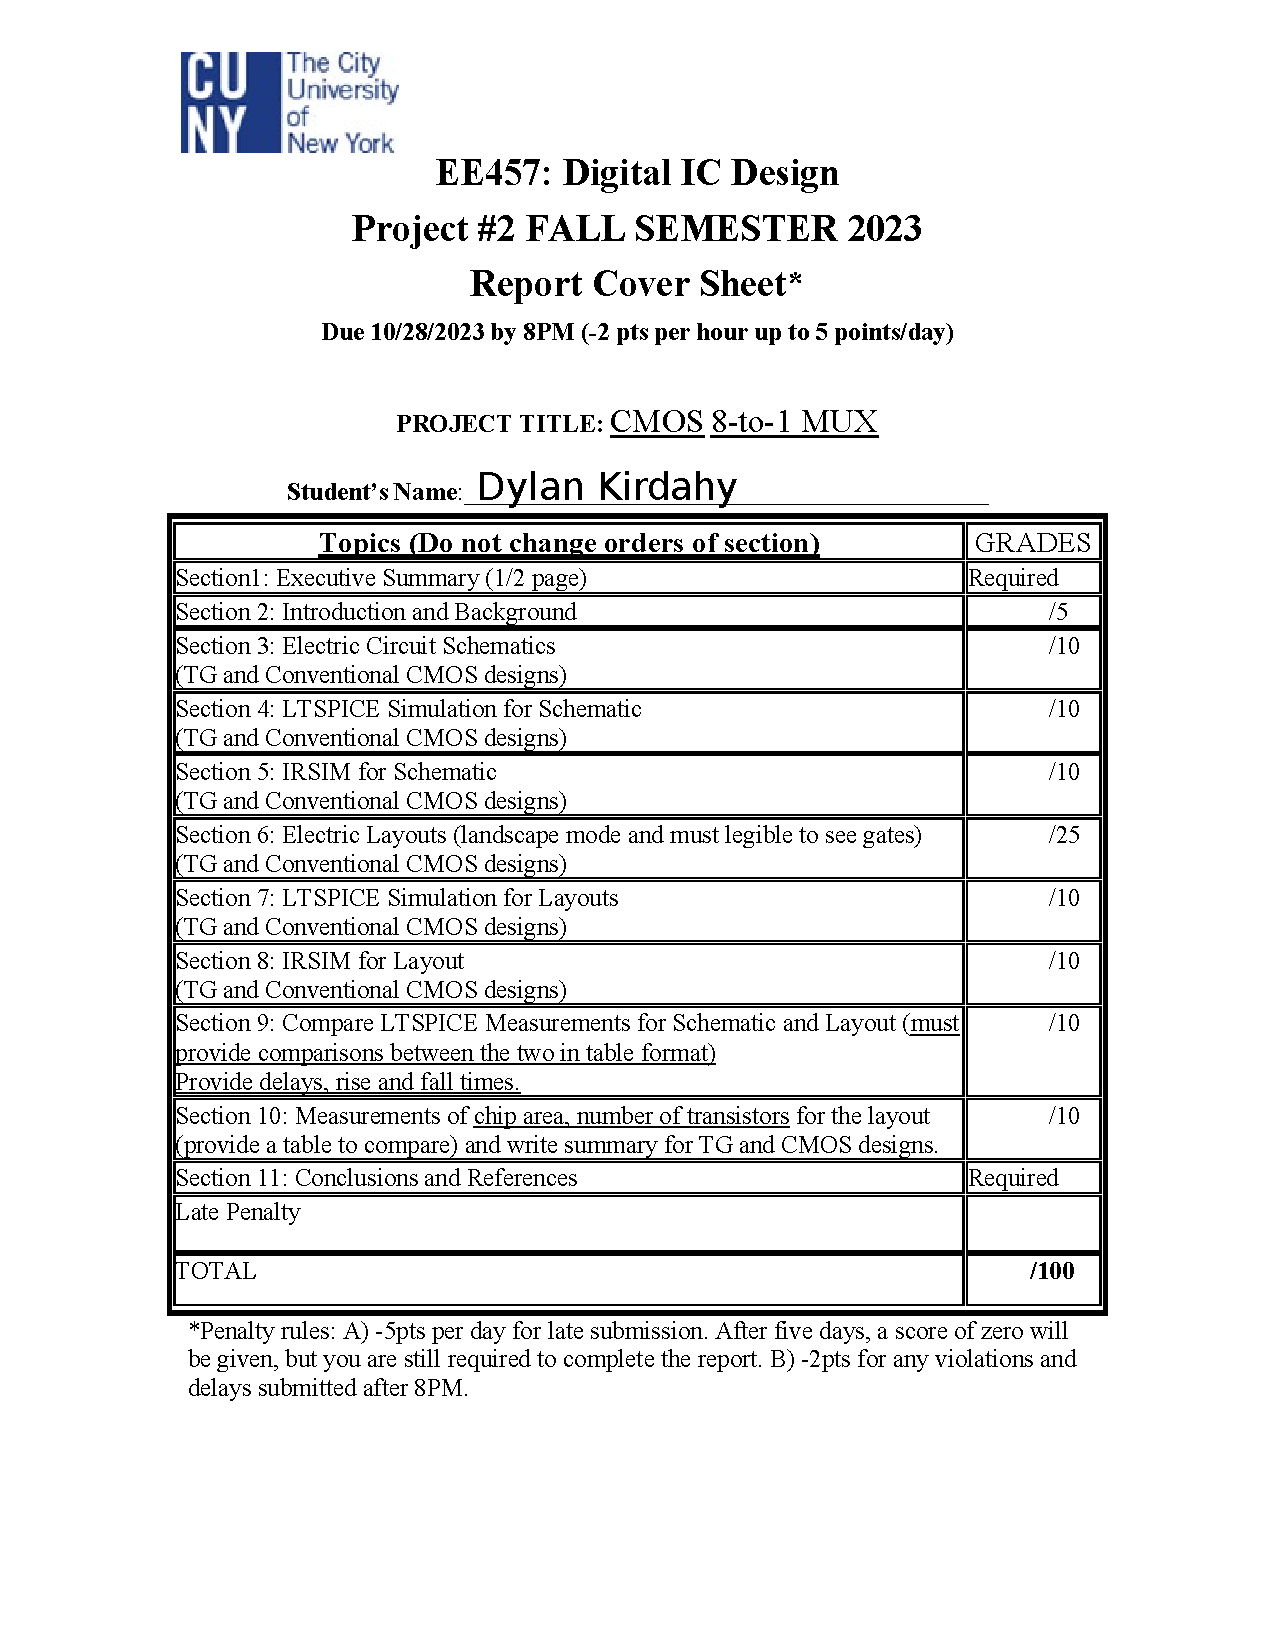
\includepdf[pages=-,scale=1,pagecommand={}]{cover-sheet.pdf}

\tableofcontents

\newpage
\pagenumbering{arabic}

\section{Executive Summary}
  \paragraph{}
  The goal of this project was to build an 8-to-1 multiplexer twice, once using transmission gates and once using ordinary CMOS logic. A multiplexer is a combinational logic circuit that allows for one of many inputs to be passed through to a single output. In this case there are 8 inputs, D0 to D7, and the state of output Y reflects the state of the input selected with the select lines S0, S1, and S2. Multiplexers have a variety of uses in digital electronics, most notably in the design of CPUs.

  \paragraph{}
  In this project, the multiplexer is realized using the software Electric, which allows us to design a schematic, layout, and icon for the multiplexer. We are also able to export the design to LTSpice in order to run in-depth simulations as well as simulate the designs with the built-in IRSIM. 

  \paragraph{}
  I designed the transmission gate multiplexer and the CMOS multiplexer with two different philosophies. For the transmission gate design, I used the method that we learned about in class, where each input has its own set of transmission gates that connect to a single node for the output. For the CMOS design, I chose to create a 2-to-1 multiplexer and then chain them together to build the 8-to-1 multiplexer. Both designs were an interesting challenge.

  \paragraph{}
  The simulation component of the project involved generating input signals and then confirming that the designs generates the expected output. In addition, various measurements can be taken within LTSpice with the \inlinecode{.meas} command. These measurements include propagation delay, rise and fall times, and average current draw.

\section{Introduction and Background}
  \paragraph{}
  The multiplexer is a combinational logic circuit that is crucial to many digital designs. Multiplexers allow us to choose which input out of a number of inputs reaches the output using select lines. They can be designed to take any number of inputs, but typically a power of two. The simplest multiplexer design is a 2-to-1 multiplexer: there are two inputs, D0 and D1, and a single output, Y, and the select line, S, determines which of the inputs reach the output. For instance, when a logic 0 is applied to S, whatever digital signal is applied to D0 is output on Y, and when a logic 1 is applied to S, the signal applied to D1 is output on Y. When one input is selected, all other inputs are ignored.

  \paragraph{}
  This logic extends to multiplexers with more inputs. A 4-bit multiplexer has four inputs and one output, and two select lines (S1 and S0) are used to select which of the four inputs is output. 00 selects D0, 01 selects D1, 10 selects D2, and 11 selects D3. Multiplexers can be designed with 8 inputs, 16 inputs, 32 inputs, etc., however in the scope of this project we are building an 8-bit multiplexer which has eight inputs and uses three select lines (S2, S1, S0) to determine which input reaches the output. An interesting side note is that multiplexers can pass an analog signal or a digital signal based on how they are designed; the CMOS design can only pass a digital signal, but the transmission gate design can pass an analog signal as well due to the transmission gates acting as closed or open switches. However, passing analog signals is outside of the scope of this project.

  \paragraph{}
  In order to create the design for our 8-to-1 multiplexer, we first need to create a function and a truth table to get a better understanding of the logic that powers the multiplexer. Since our CMOS design is based on a 2-to-1 multiplexer, we will start there. The function for the 2-to-1 multiplexer is as follows:

  \[Y=\overline{S}\cdot D_0+S\cdot D_1\]

  \paragraph{}
  The working principle is that when $S=0$ the output is $Y=D_0$ and when $S=1$ the output is $Y=D_1$. The truth table for this function is provided below in Table \ref{table:21mux}.

  \begin{table}[H]
    \centering
    \footnotesize
    \begin{tabular}{|c|c|}
      \hline
      \textbf{S} & \textbf{Y}   \\
      \hline
      0 & D$_0$ \\
      \hline
      1 & D$_1$ \\
      \hline
   \end{tabular}
    \caption{Truth Table for the 2-to-1 multiplexer.}
    \label{table:21mux}
  \end{table}

  \paragraph{}
  This working principle can be applied to the 8-to-1 multiplexer as well. The function for the 8-to-1 multiplexer is as follows:

  \[Y = \bar{S_2} \cdot \bar{S_1} \cdot \bar{S_0} \cdot D_0 + \bar{S_2} \cdot \bar{S_1} \cdot S_0 \cdot D_1 + \bar{S_2} \cdot S_1 \cdot \bar{S_0} \cdot D_2 + \bar{S_2} \cdot S_1 \cdot S_0 \cdot D_3 + S_2 \cdot \bar{S_1} \cdot \bar{S_0} \cdot D_4 + S_2 \cdot \bar{S_1} \cdot S_0 \cdot D_5 + S_2 \cdot S_1 \cdot \bar{S_0} \cdot D_6 + S_2 \cdot S_1 \cdot S_0 \cdot D_7
\]

  \paragraph{}
  The truth table for the 8-to-1 multiplexer is shown below in Table \ref{table:81mux}.


  \begin{table}[H]
    \centering
    \footnotesize
    \begin{tabular}{|c|c|c|c|}
      \hline
      \textbf{S$_2$} & \textbf{S$_1$} & \textbf{S$_0$} & \textbf{Y}   \\
      \hline
      0 & 0 & 0 & D$_0$ \\
      \hline
      0 & 0 & 1 & D$_1$ \\
      \hline
      0 & 1 & 0 & D$_2$ \\
      \hline
      0 & 1 & 1 & D$_3$ \\
      \hline
      1 & 0 & 0 & D$_4$ \\
      \hline
      1 & 0 & 1 & D$_5$ \\
      \hline
      1 & 1 & 0 & D$_6$ \\
      \hline
      1 & 1 & 1 & D$_7$ \\
      \hline
   \end{tabular}
    \caption{Truth Table for the 8-to-1 multiplexer.}
    \label{table:81mux}
  \end{table}

  \paragraph{}
  The symbol for the 8-to-1 multiplexer, designed in Electric to represent the schematic, is shown in Figure \ref{fig:symbol}.


  \begin{figure}[H]
    \centering
    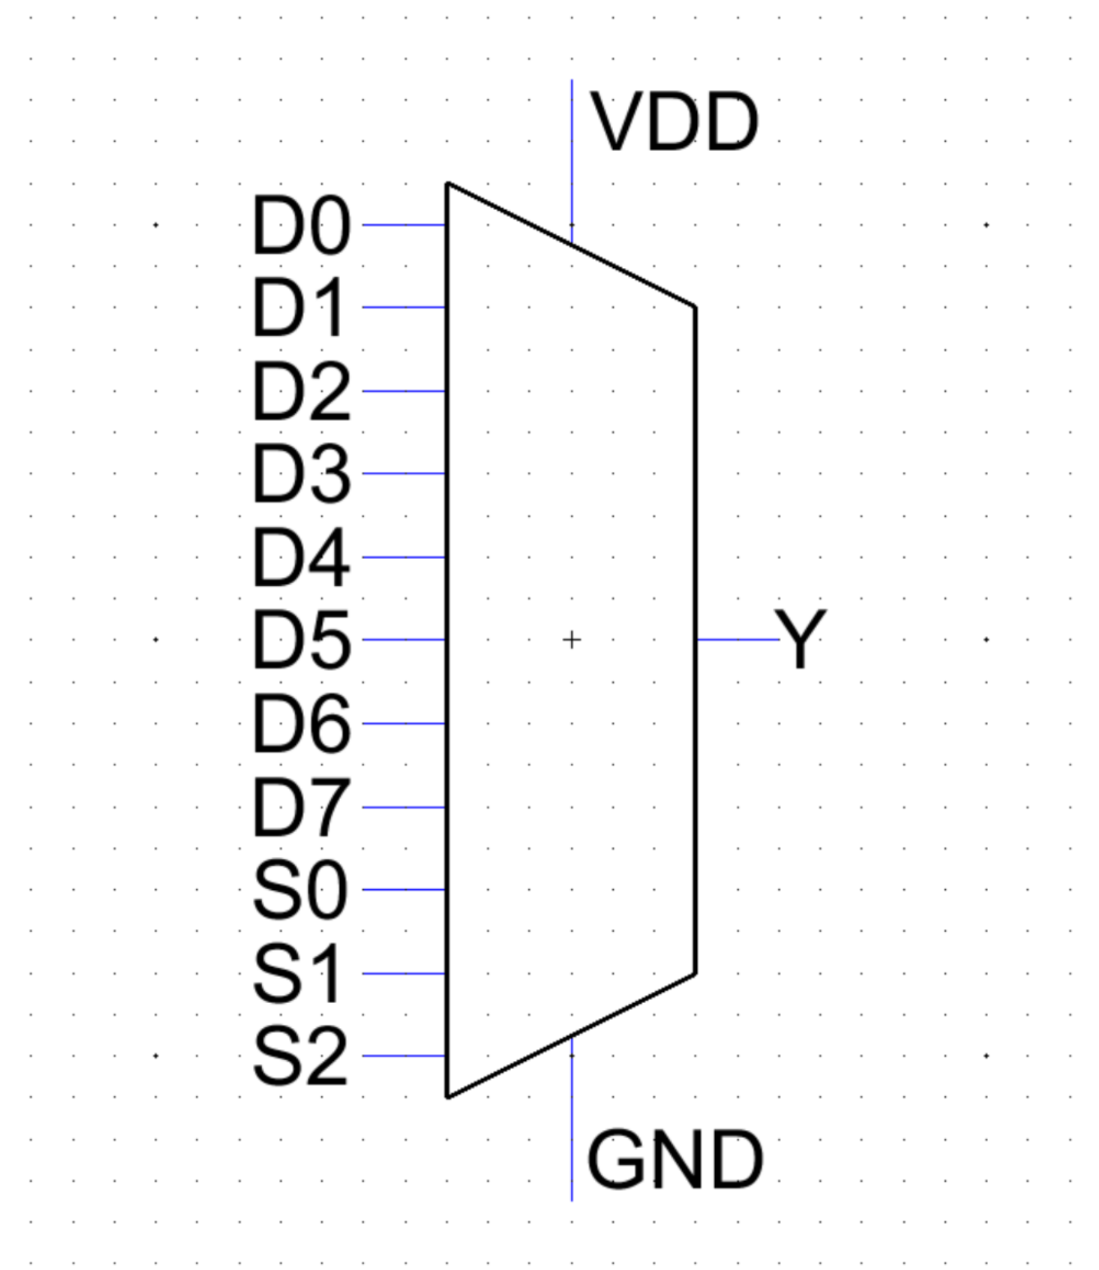
\includegraphics[width=0.5\linewidth, frame]{screenshots/symbol.png}
    \caption{The symbol for the 8-to-1 multiplexer designed in Electric.}
    \label{fig:symbol}
  \end{figure}



  \paragraph{}
  As mentioned before, the transmission gate design was made with 8 separate sets of three transmission gates (for S2, S1, and S0). However, the CMOS design was built by chaining together seven 2-to-1 multiplexers. The configuration of these 2-to-1 multiplexers in order to make the 8-to-1 multiplexer is shown in Figure \ref{fig:mux}.


  \begin{figure}[H]
    \centering
    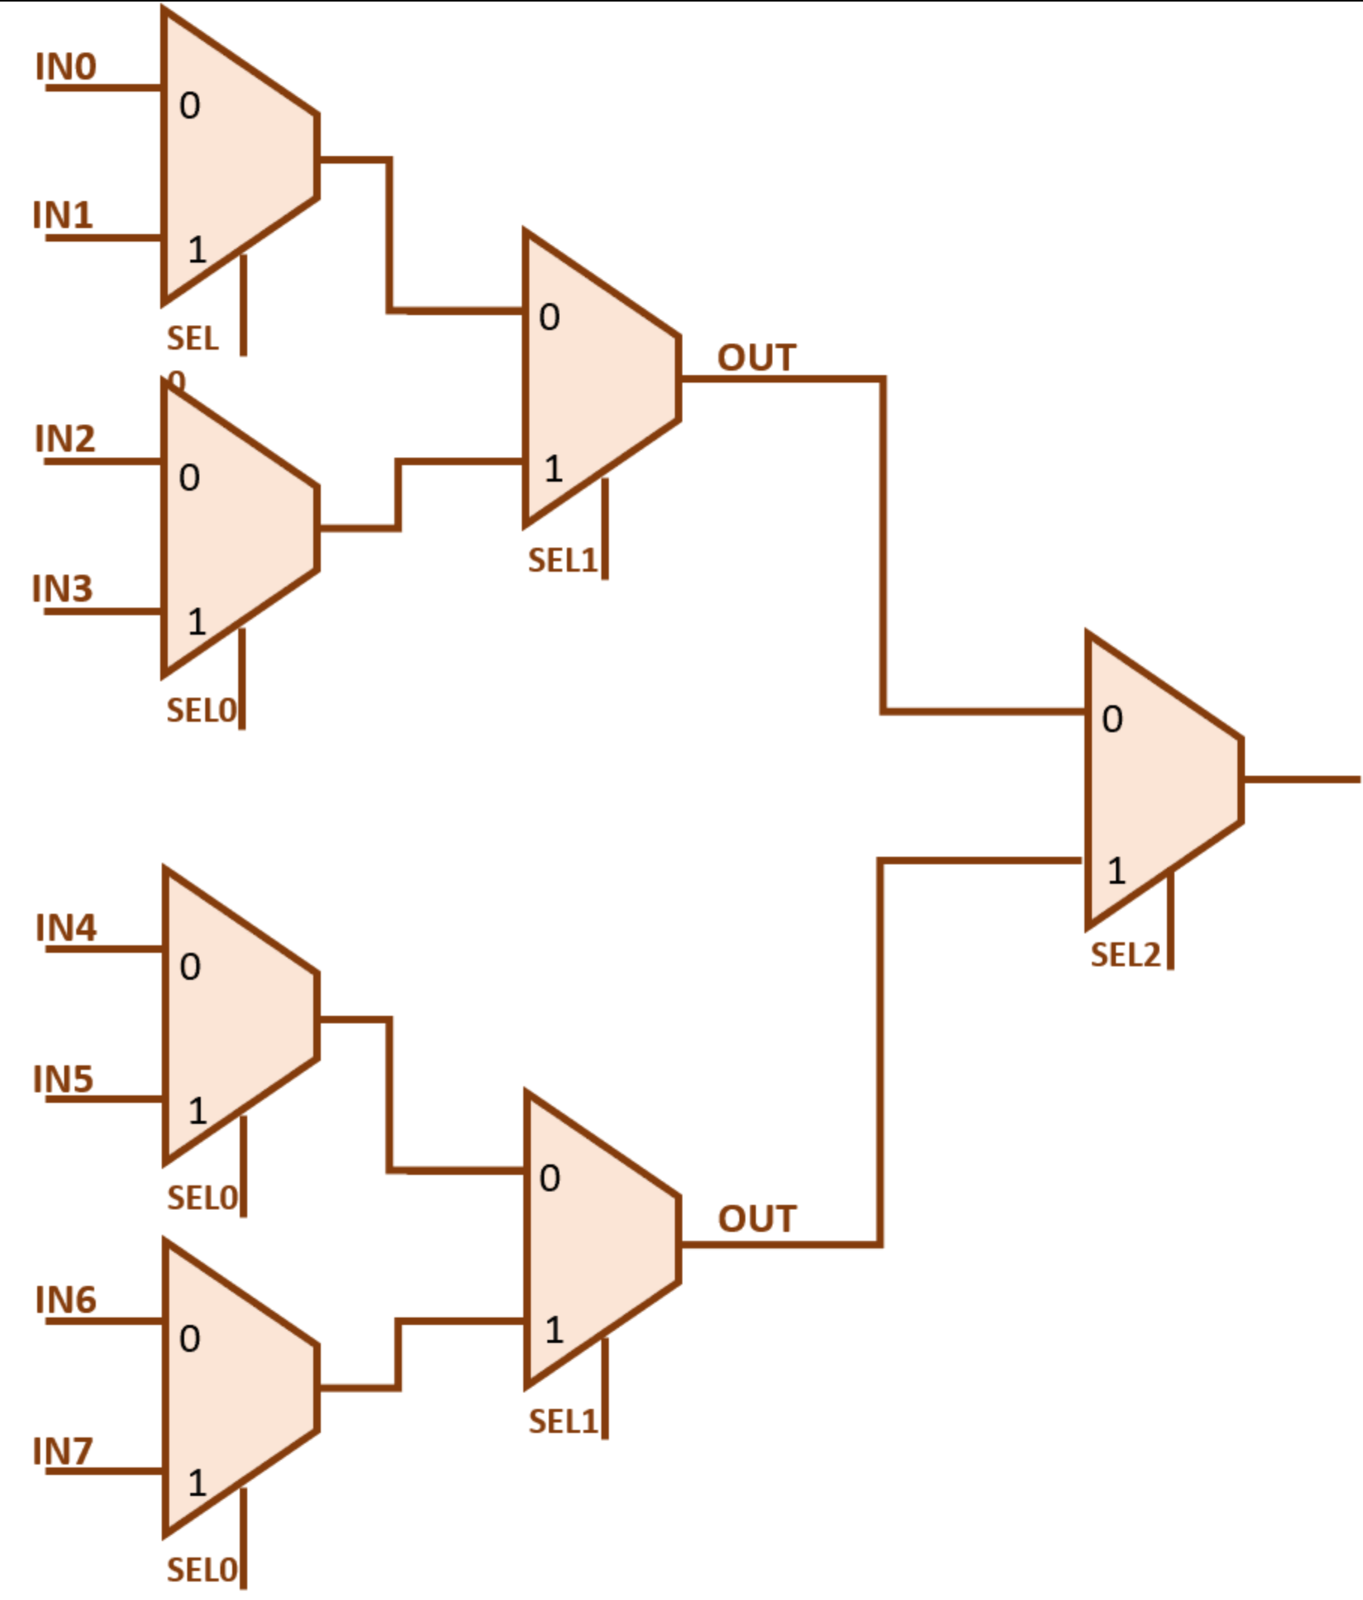
\includegraphics[width=0.5\linewidth, frame]{images/mux.png}
    \caption{The configuration of seven 2-to-1 multiplexers to create a single 8-to-1 multiplexer.}
    \label{fig:mux}
  \end{figure}

  In order to implement this, we first need to create the 2-to-1 multiplexer. I started with the function $Y=\overline{S}\cdot D_0+S\cdot D_1$ and implemented it with CMOS logic. Since CMOS logic outputs an inverted signal, we can do one of two things: either invert the function and then implement that, or add an inverter at the end. I chose to add an inverter at the end, since inverting the whole function would involve inverting both D0 and D1 in addition to S. Adding an inverter at the end means we only need two inverters instead of three. The sketch I drew of the schematic is shown in Figure \ref{fig:21schem}.


  \begin{figure}[H]
    \centering
    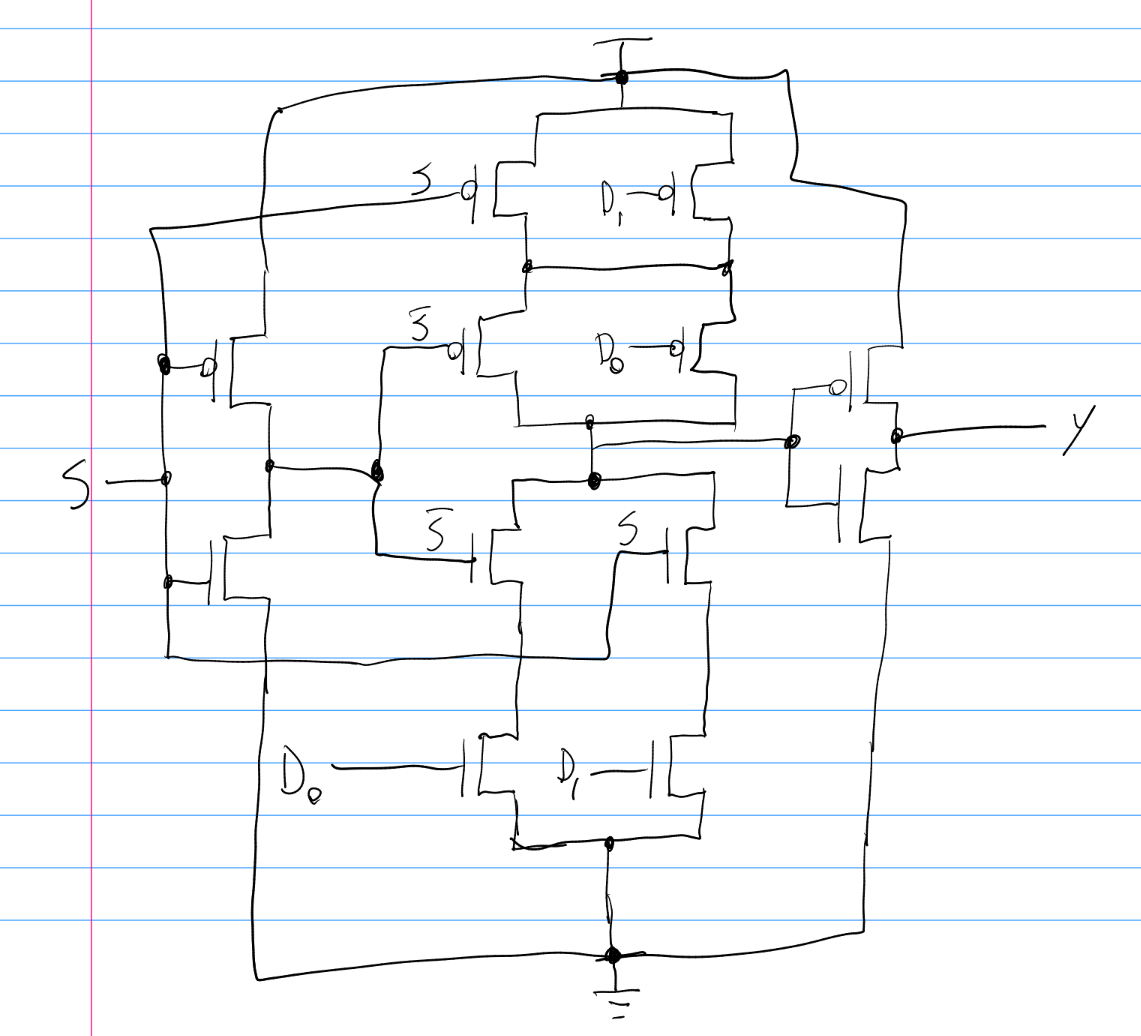
\includegraphics[width=0.5\linewidth, frame]{screenshots/21schem.png}
    \caption{A sketch of the schematic for a single 2-to-1 multiplexer.}
    \label{fig:21schem}
  \end{figure}

  \paragraph{}
  The next step was to determine an Euler's Path from the sketch. The Euler's Paths that I determined are shown in Figure \ref{fig:euler}.


  \begin{figure}[H]
    \centering
    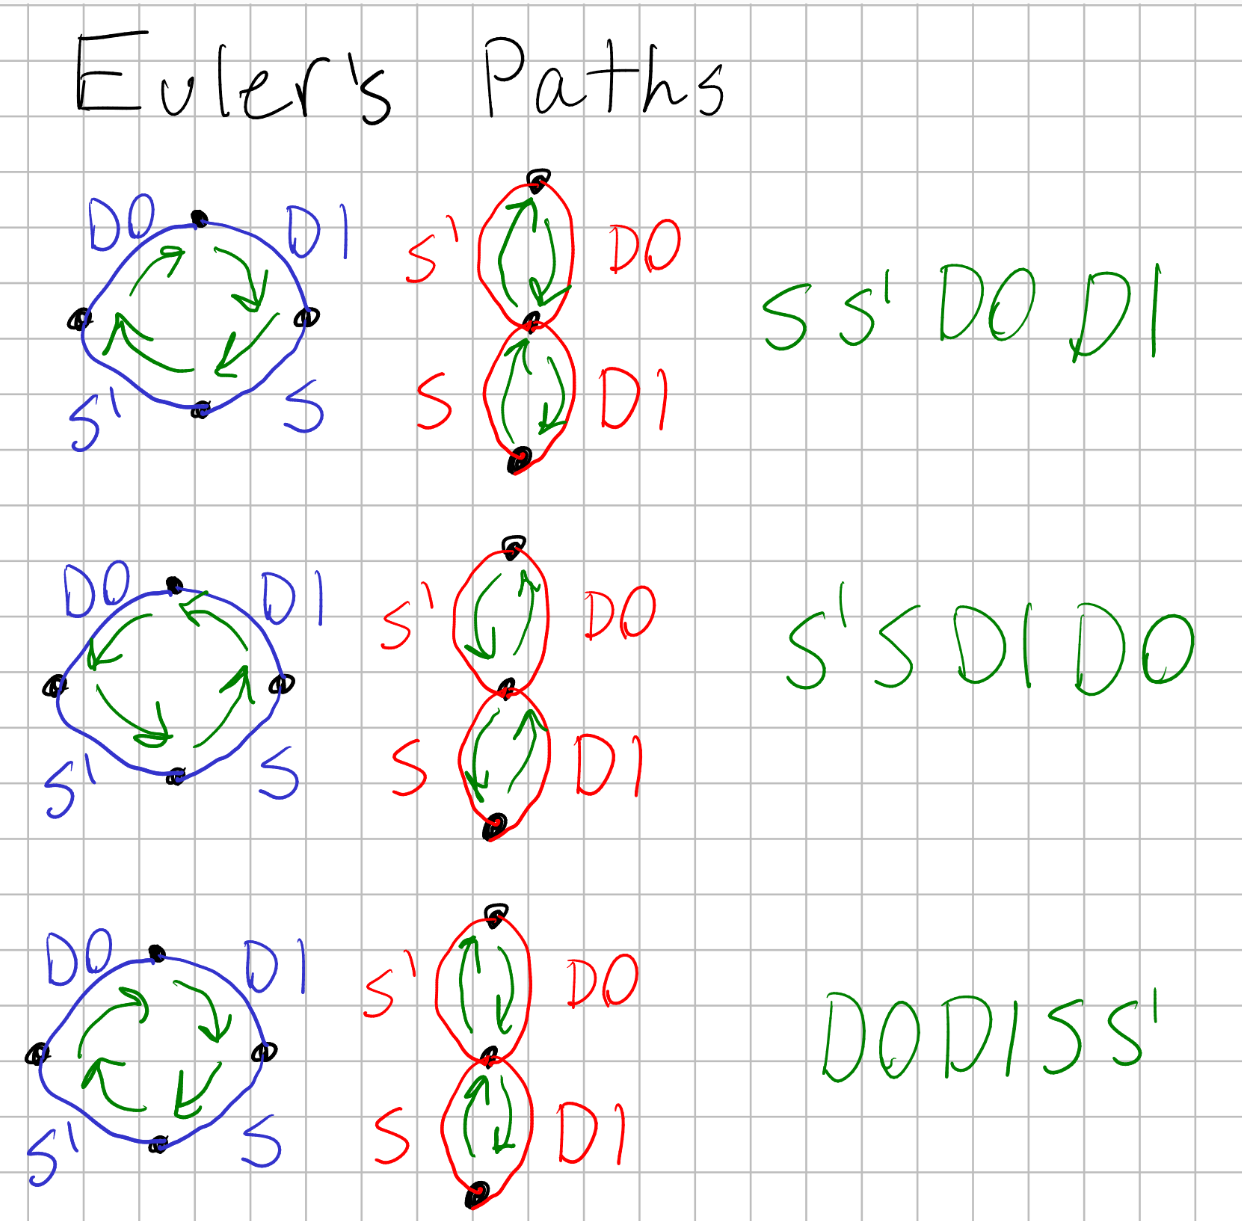
\includegraphics[width=0.5\linewidth, frame]{screenshots/euler.png}
    \caption{A few Euler's Paths for the 2-to-1 multiplexer.}
    \label{fig:euler}
  \end{figure}

  \paragraph{}
  I decided to use the path $\overline{S},S,D_1,D_0$ since it seemed to be the most space efficient to me. The stick diagram I sketched based on the Euler's Path chosen is shown in Figure \ref{fig:stick}.

  \begin{figure}[H]
    \centering
    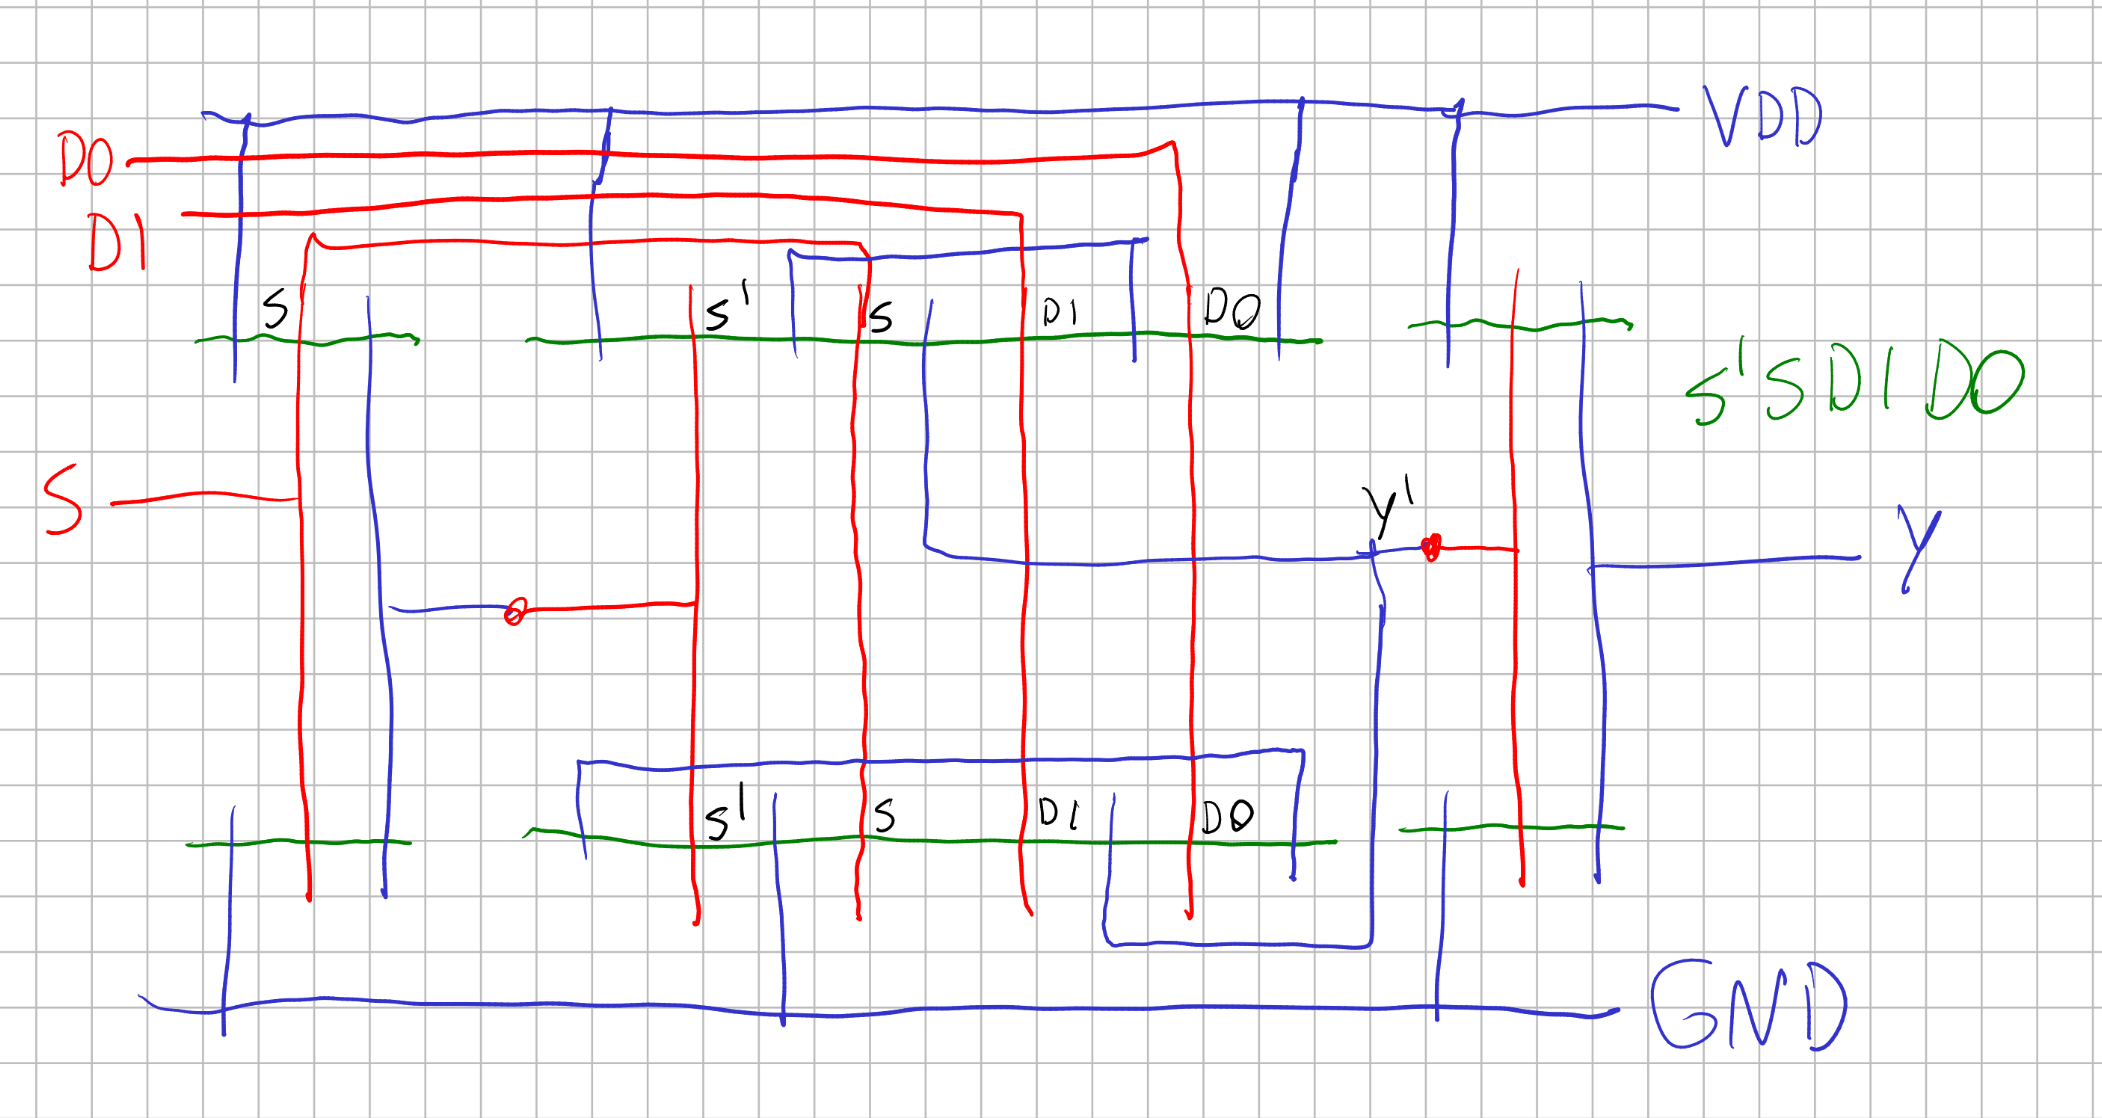
\includegraphics[width=0.7\linewidth, frame]{screenshots/stick.png}
    \caption{The stick diagram for the 2-to-1 multiplexer.}
    \label{fig:stick}
  \end{figure}


  \paragraph{}
  We now have all of the information we need to begin the design of both the transmission gate and CMOS multiplexers.



\section{Electric Circuit Schematics}
  \paragraph{}
  This section details the design of the schematics for the transmission gate and CMOS designs of the multiplexer.

  \subsection{Transmission Gate Schematic}
    \paragraph{}
    The schematic for the transmission gate design of the 8-to-1 multiplexer is shown in Figure \ref{fig:tgschem1}. The design works by giving each input (D0 through D7) its own set of three transmission gates. Each transmission gate corresponds to one of the select pins, S2, S1, or S0. As shown in table \ref{table:81mux}, each input corresponds to a specific combination of inputs to the select line. When that combination of the inputs is applied to the select line, the corresponding D input (and only that input) is connected to the output. Since there are eight inputs, there are eight sets of three transmission gates. A closer look at the sets of transmission gates can be seen in Figure \ref{fig:tgschem2}. Since each transmission gate requires an inverted signal as well as a non-inverted signal to operate, each select pin has its own inverter, which can be seen more clearly in Figure \ref{fig:tgschem3}.



    \begin{figure}[H]
      \centering
      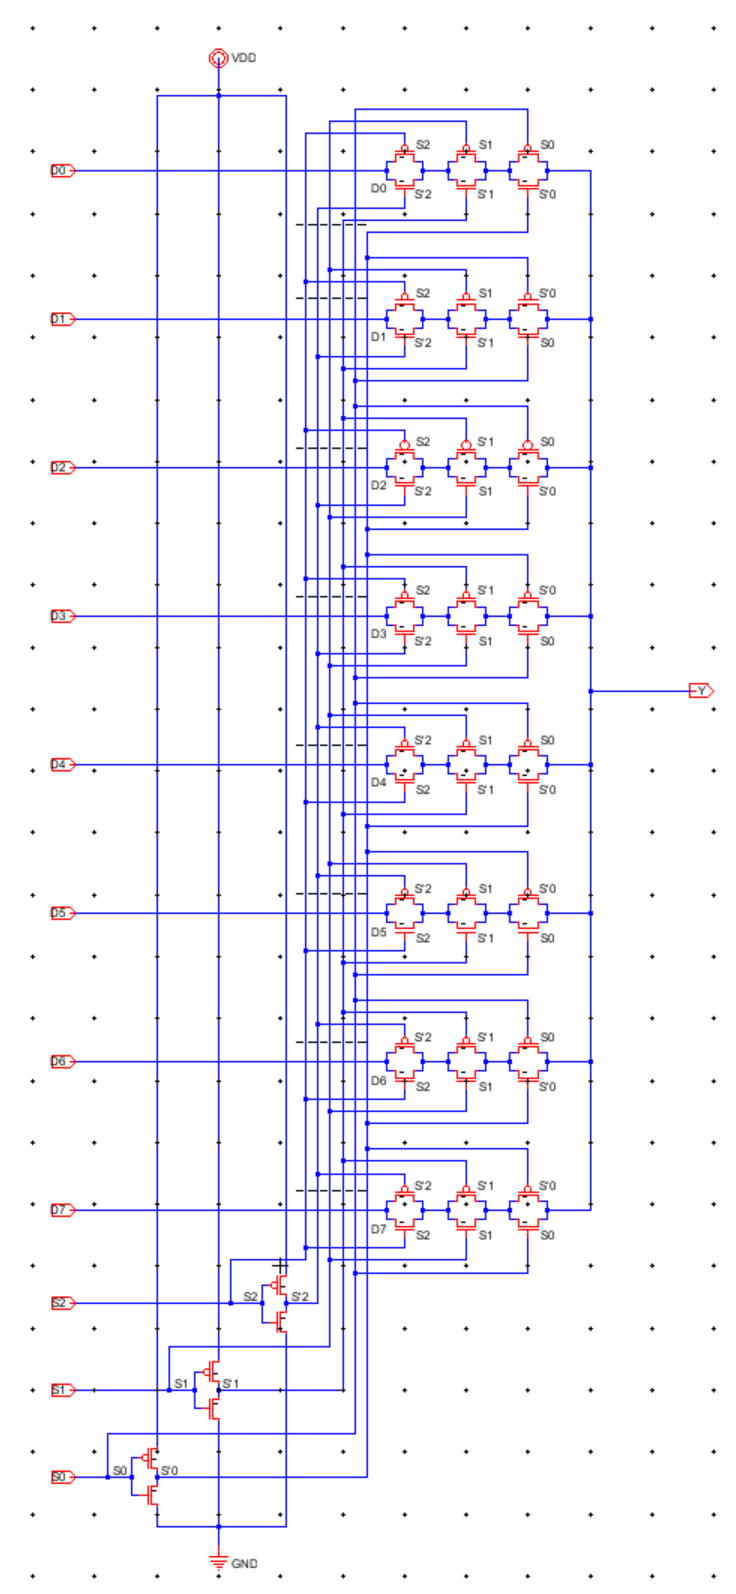
\includegraphics[width=0.7\linewidth, frame]{screenshots/tg/schem/schem1.png}
      \caption{The schematic in Electric for the transmission gate design.}
      \label{fig:tgschem1}
    \end{figure}

    \begin{figure}[H]
      \centering
      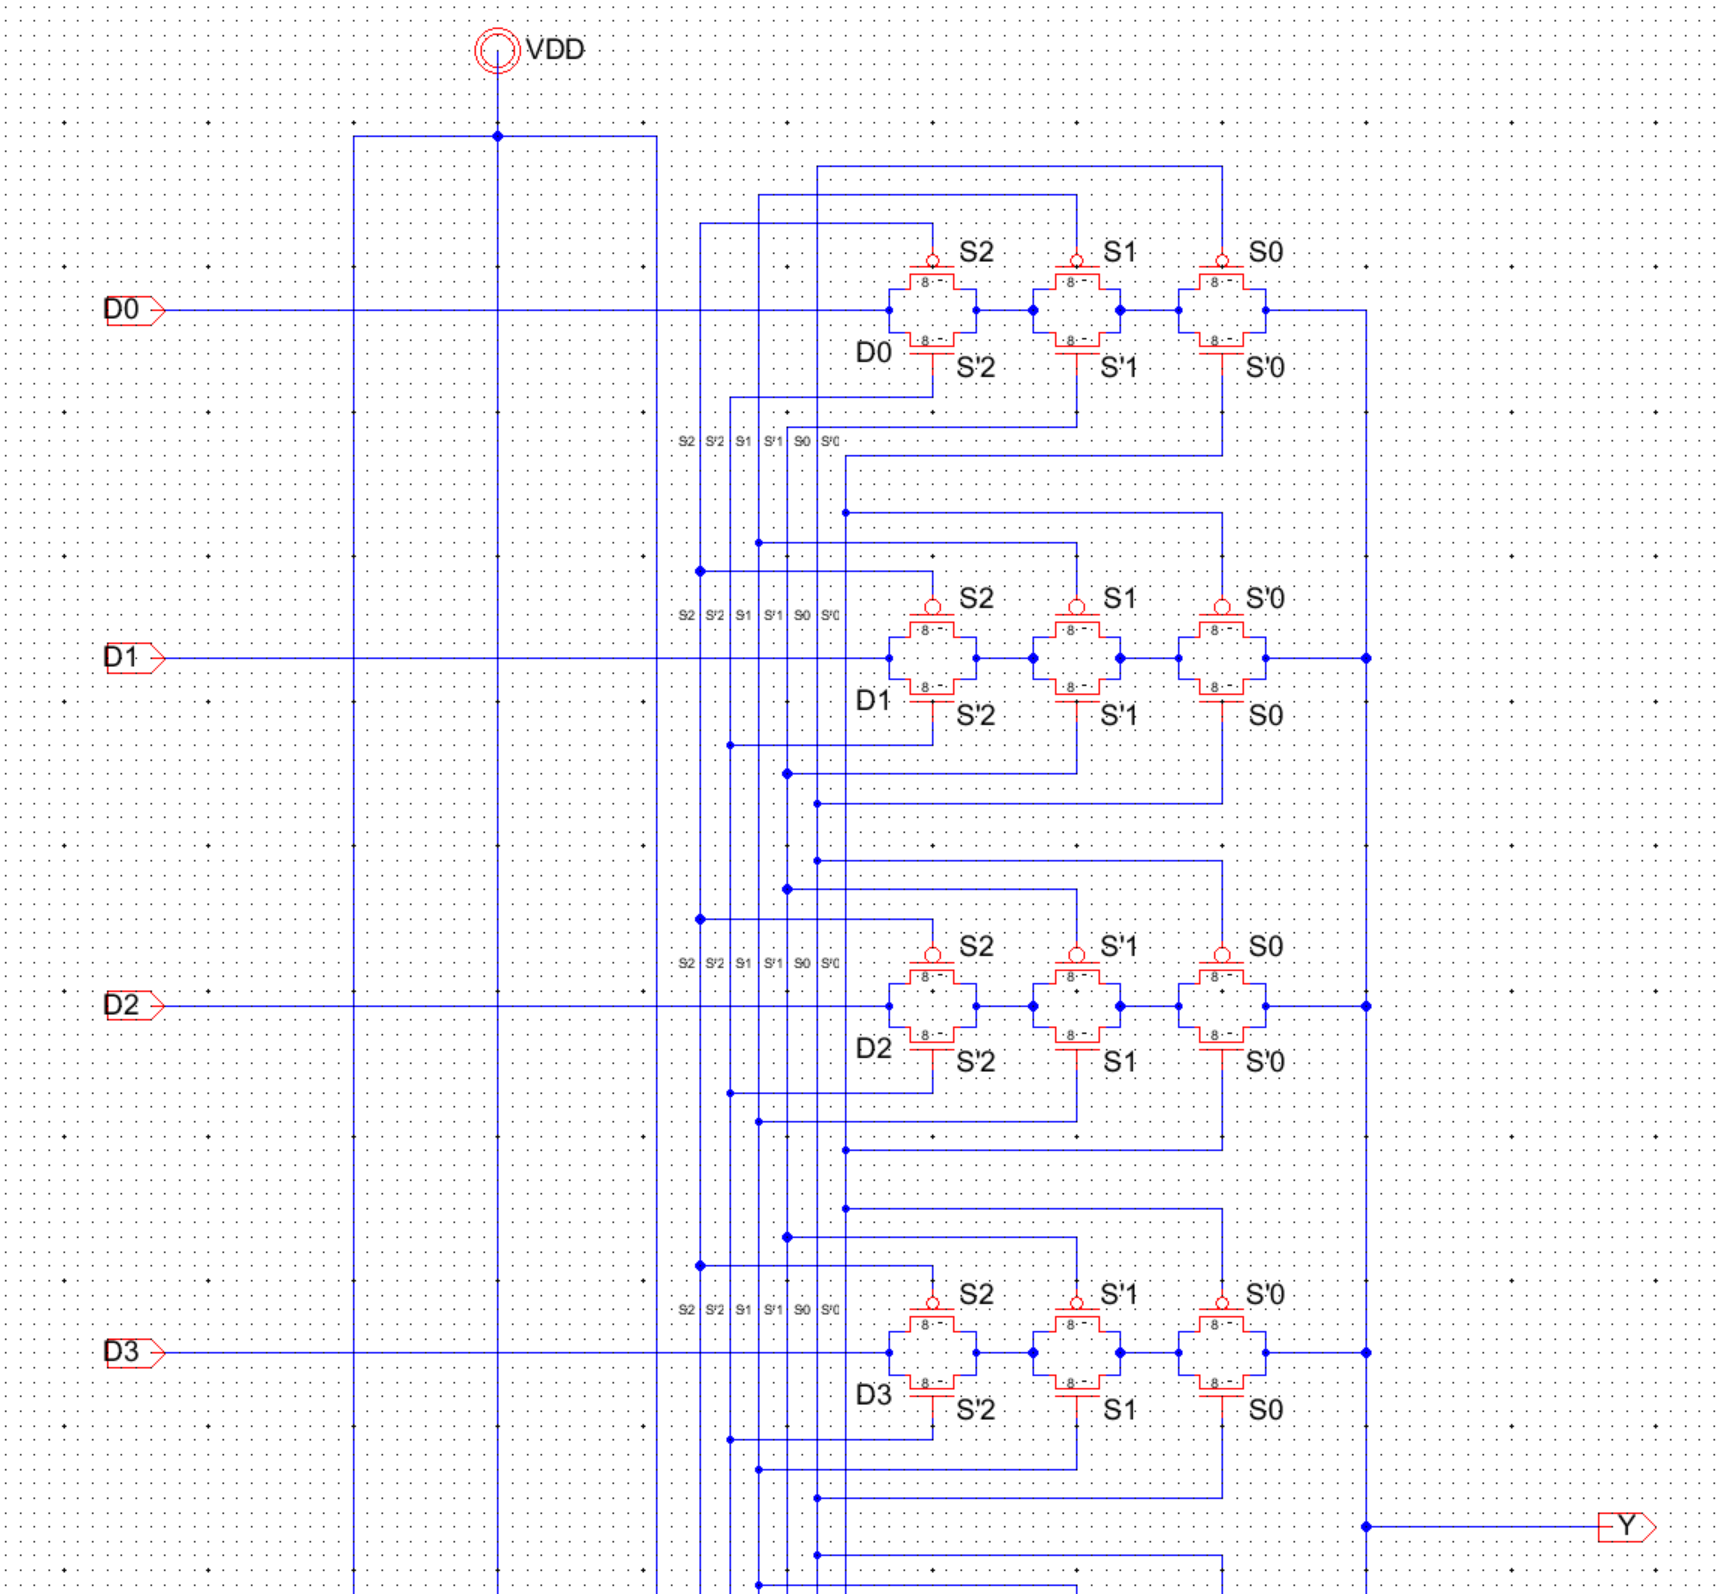
\includegraphics[width=0.6\linewidth, frame]{screenshots/tg/schem/schem2.png}
      \caption{A close up of the schematic showing the sets of transmission gates.}
      \label{fig:tgschem2}
    \end{figure}

    \begin{figure}[H]
      \centering
      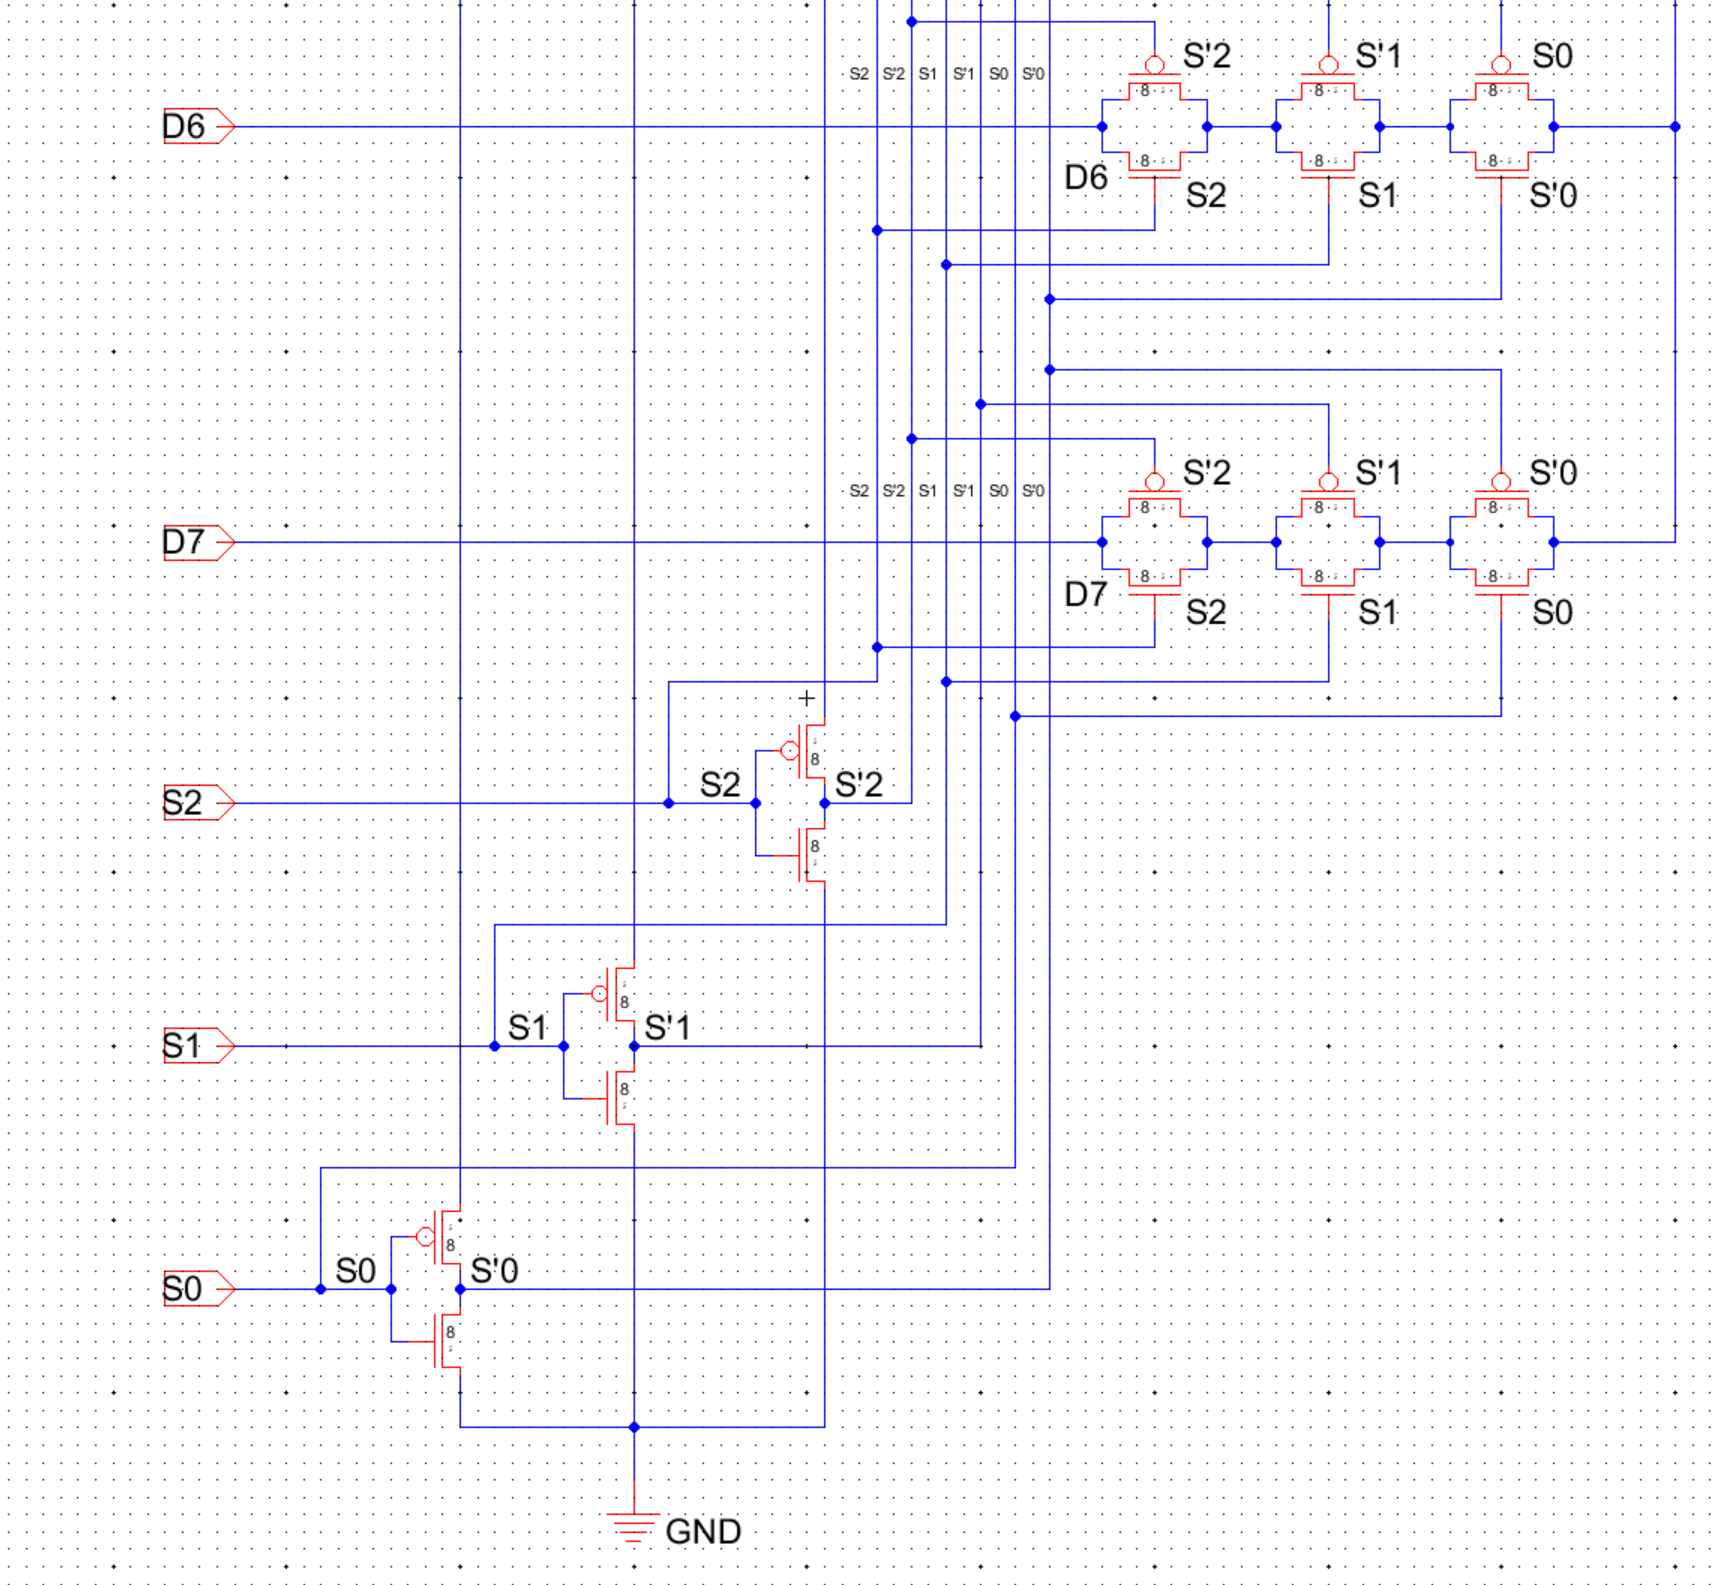
\includegraphics[width=0.6\linewidth, frame]{screenshots/tg/schem/schem3.png}
      \caption{A close up of the schematic showing the inverters which invert the select pins.}
      \label{fig:tgschem3}
    \end{figure}


    Figure \ref{fig:tgschemdrc} shows that the schematic passes the DRC check.


    \begin{figure}[H]
      \centering
      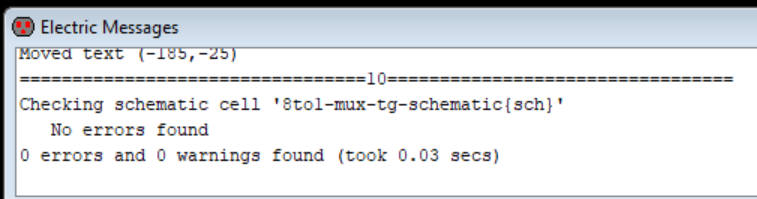
\includegraphics[width=0.6\linewidth, frame]{screenshots/tg/schem/drc.png}
      \caption{The DRC check for the transmission gate schematic.}
      \label{fig:tgschemdrc}
    \end{figure}


  \subsection{CMOS Schematic}
    \paragraph{}
    The schematic for the CMOS design of the 8-to-1 multiplexer is simply the 2-to-1 multiplexer schematic sketched in Figure \ref{fig:21schem} repeated seven times in the configuration shown in Figure \ref{fig:mux}. However, there is one change. I realized that having an inverter on the output of each of the 2-to-1 multiplexer was redundant. Only the last stage needs an inverter. This is because while the first stage inverts the output (due to CMOS logic outputting an inverted signal), the second stage will invert it again, cancelling out the first inversion. This saves 12 transistors in the final design. The full schematic is shown in Figure \ref{fig:cmosschem1}. A close up of the first two stages of the multiplexer is shown in Figure \ref{fig:cmosschem2}. A close up of the last stage is shown in Figure \ref{fig:cmosschem3}.


    \begin{figure}[H]
      \centering
      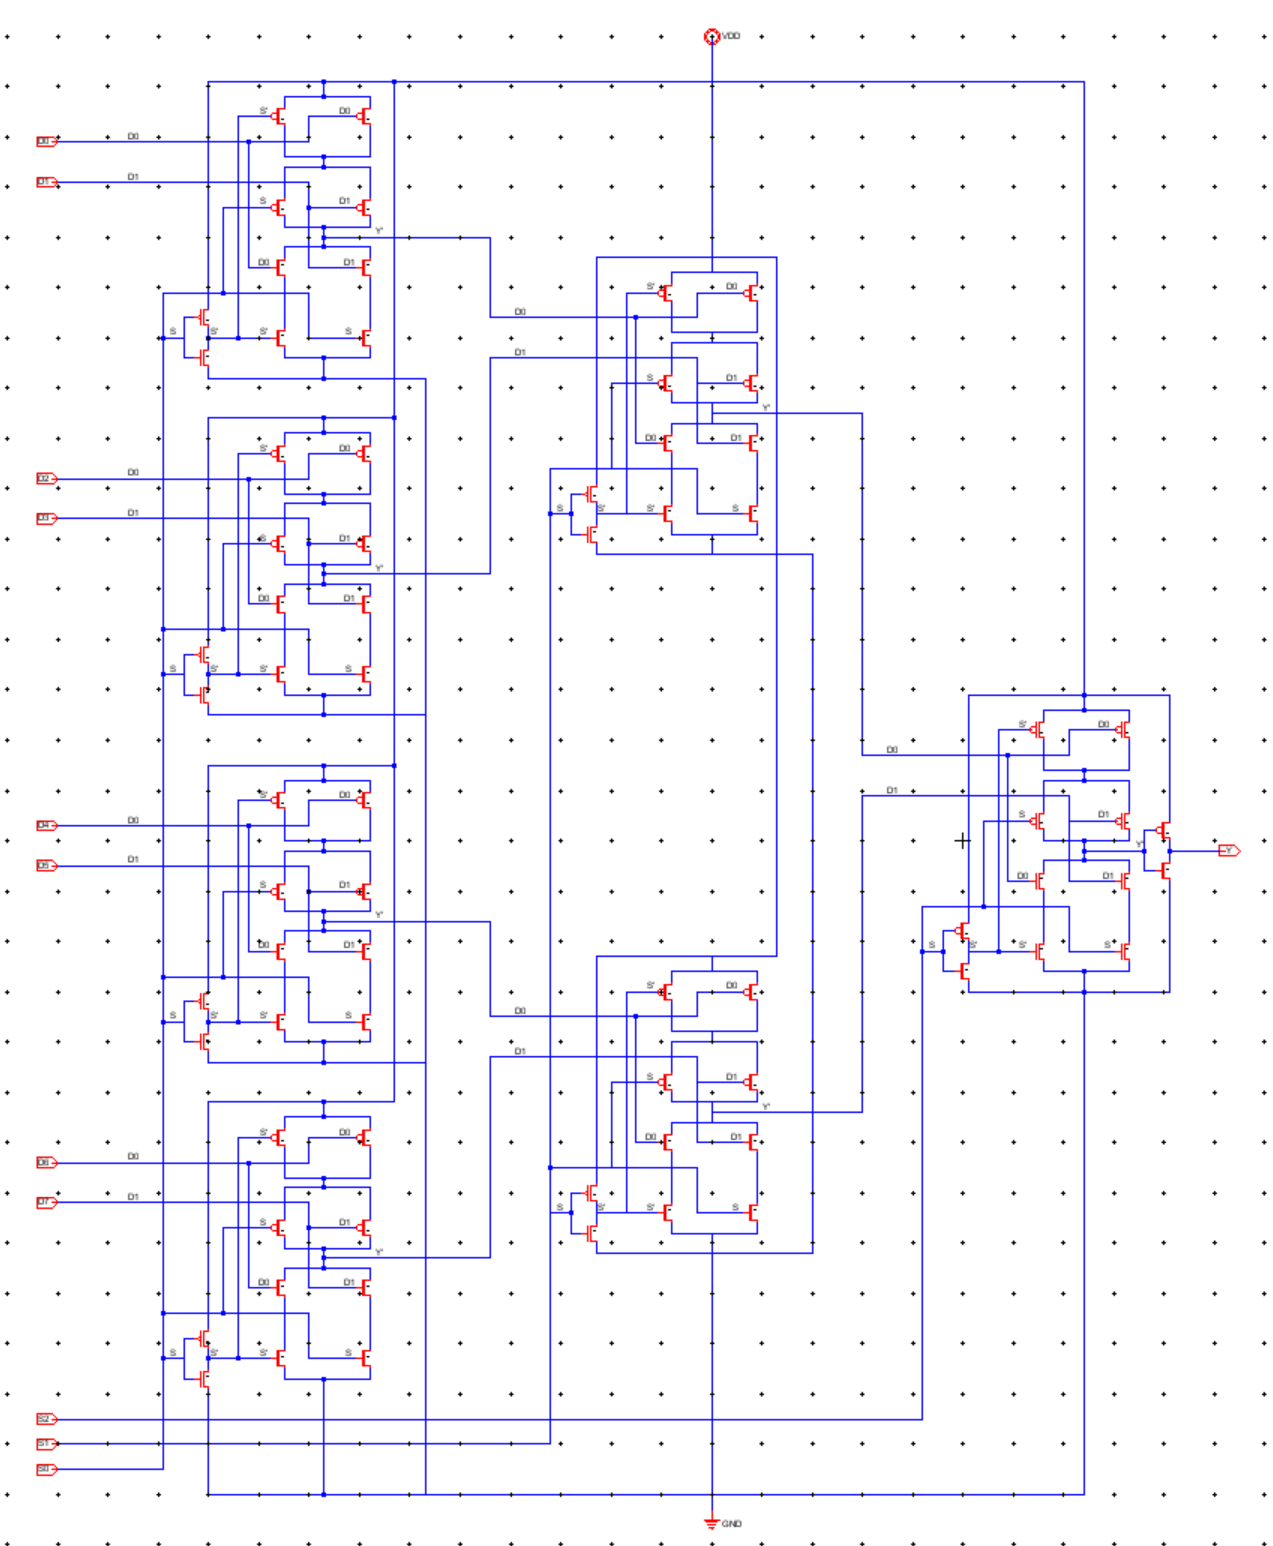
\includegraphics[width=0.9\linewidth, frame]{screenshots/cmos/schem/schem1.png}
      \caption{The schematic in Electric for the CMOS design.}
      \label{fig:cmosschem1}
    \end{figure}


    \begin{figure}[H]
      \centering
      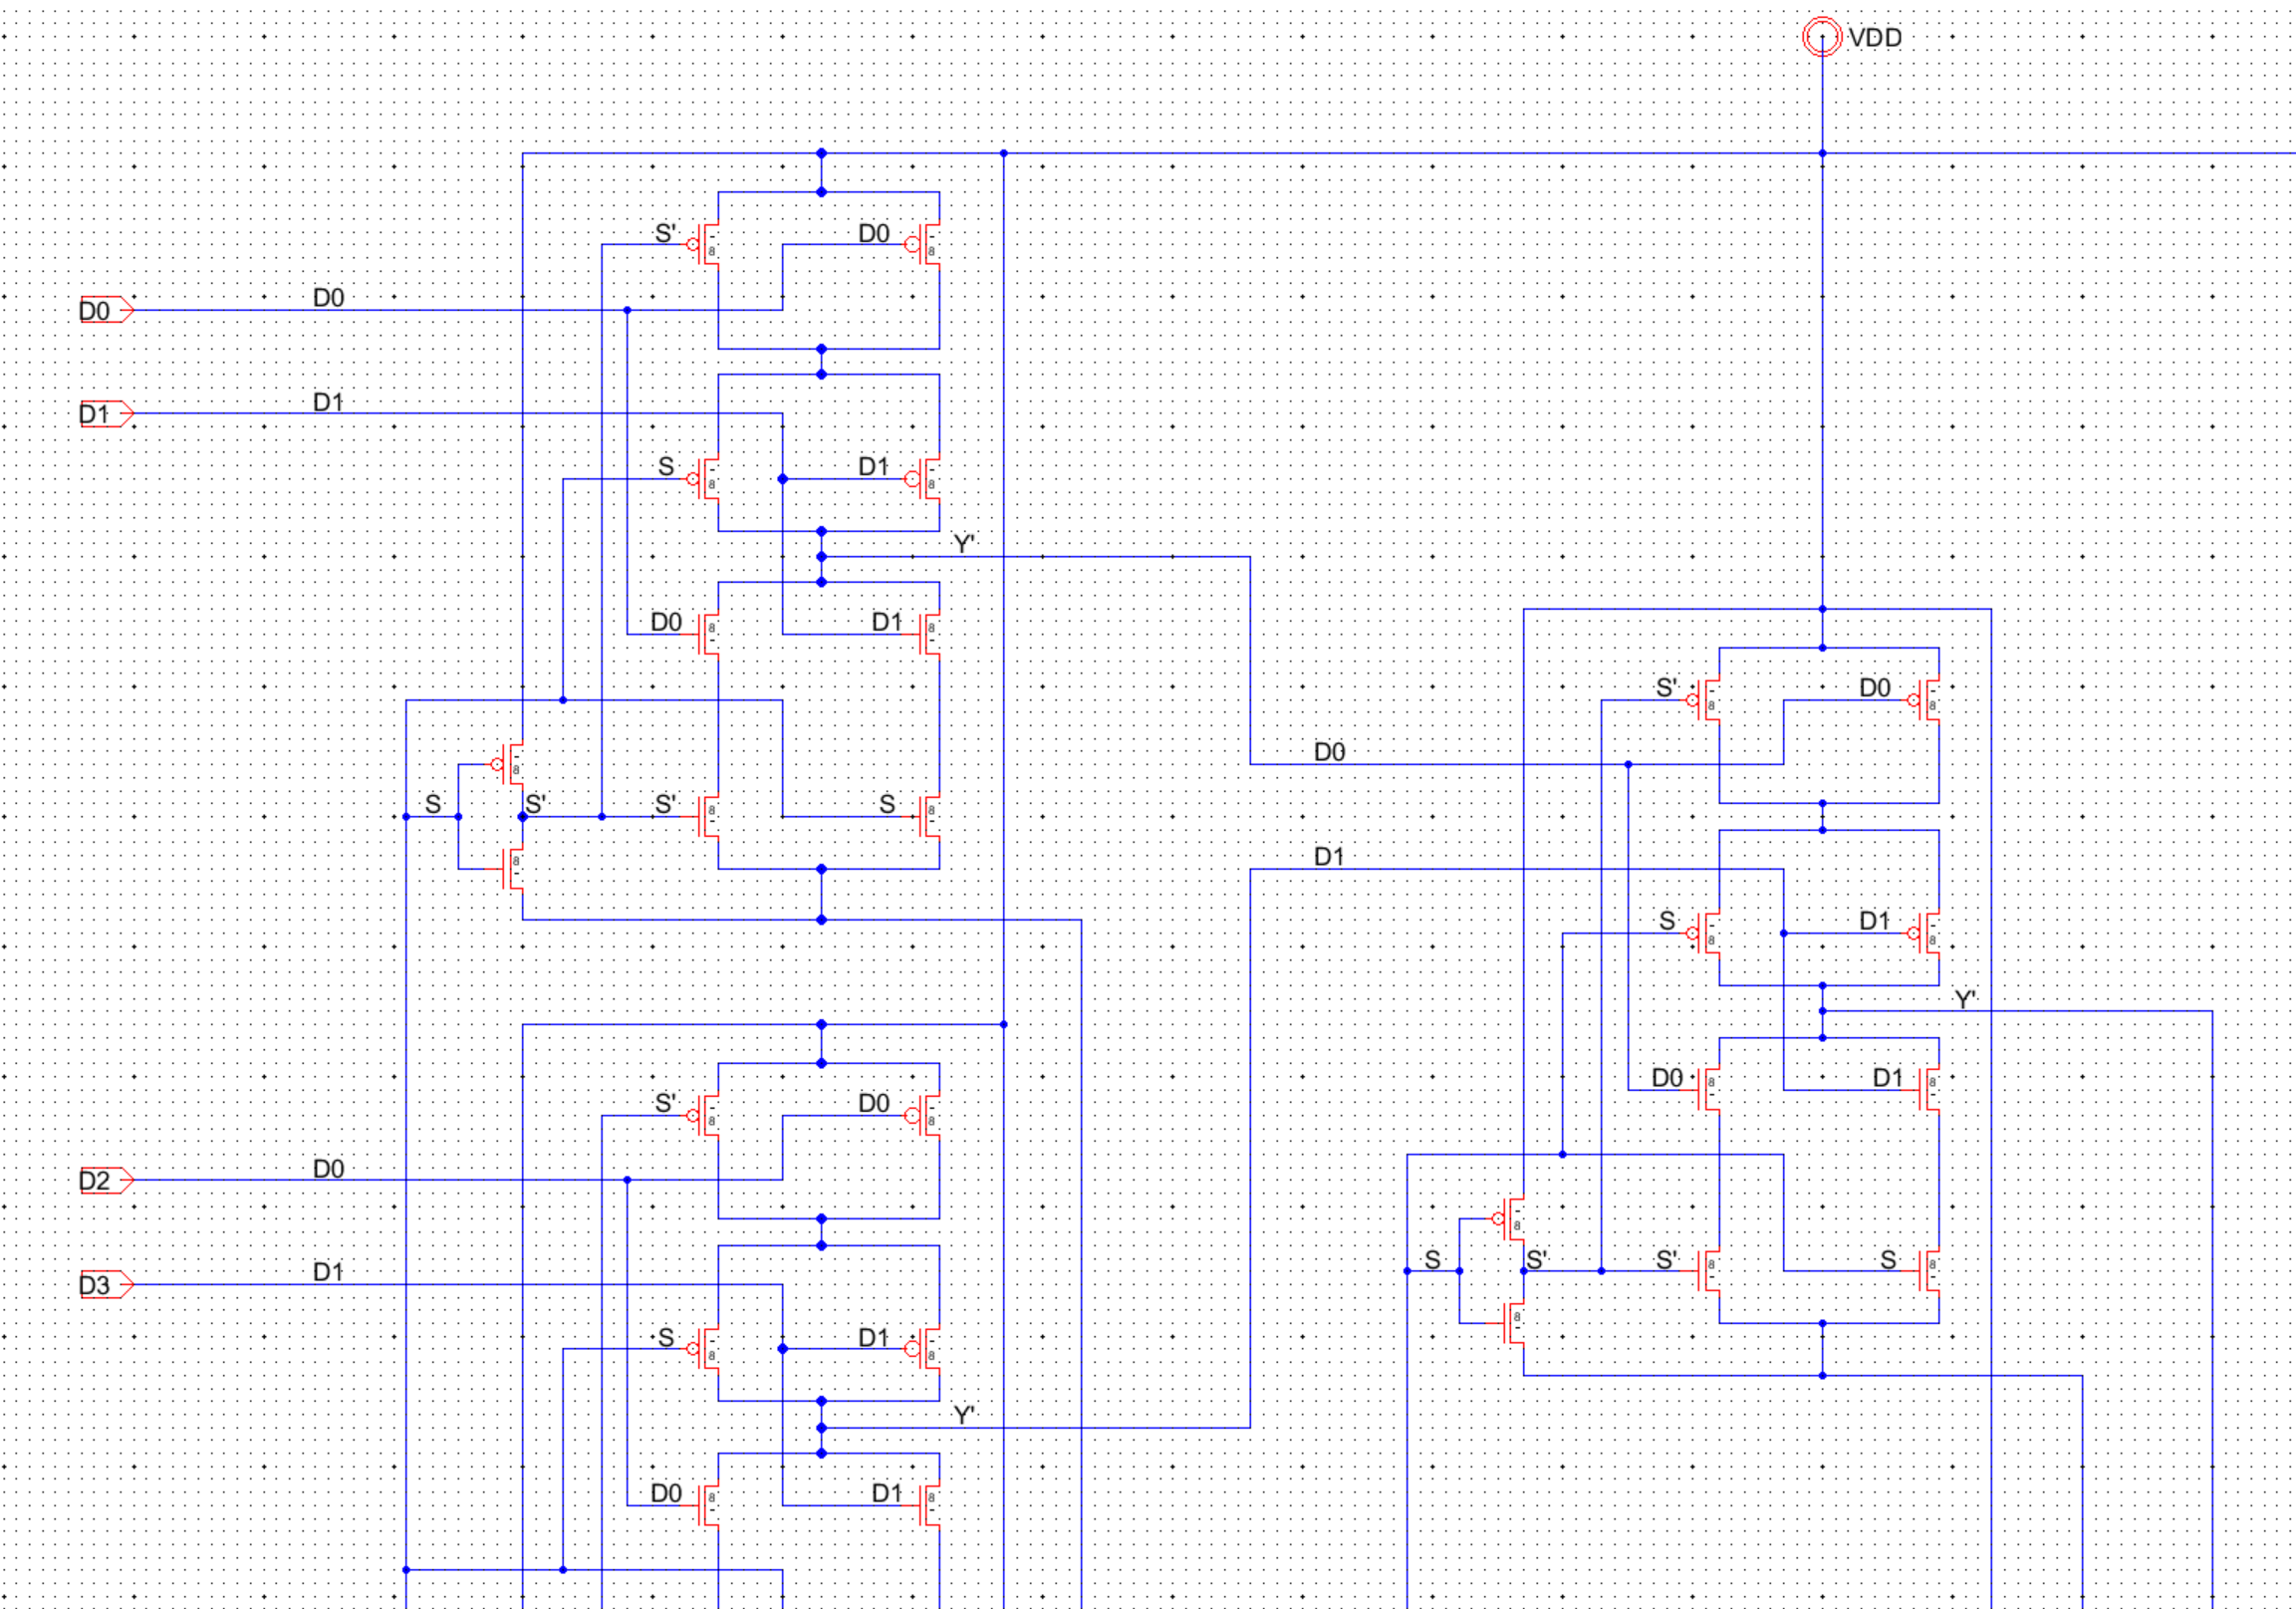
\includegraphics[width=0.9\linewidth, frame]{screenshots/cmos/schem/schem2.png}
      \caption{A close up of the schematic showing the first two stages.}
      \label{fig:cmosschem2}
    \end{figure}

    \begin{figure}[H]
      \centering
      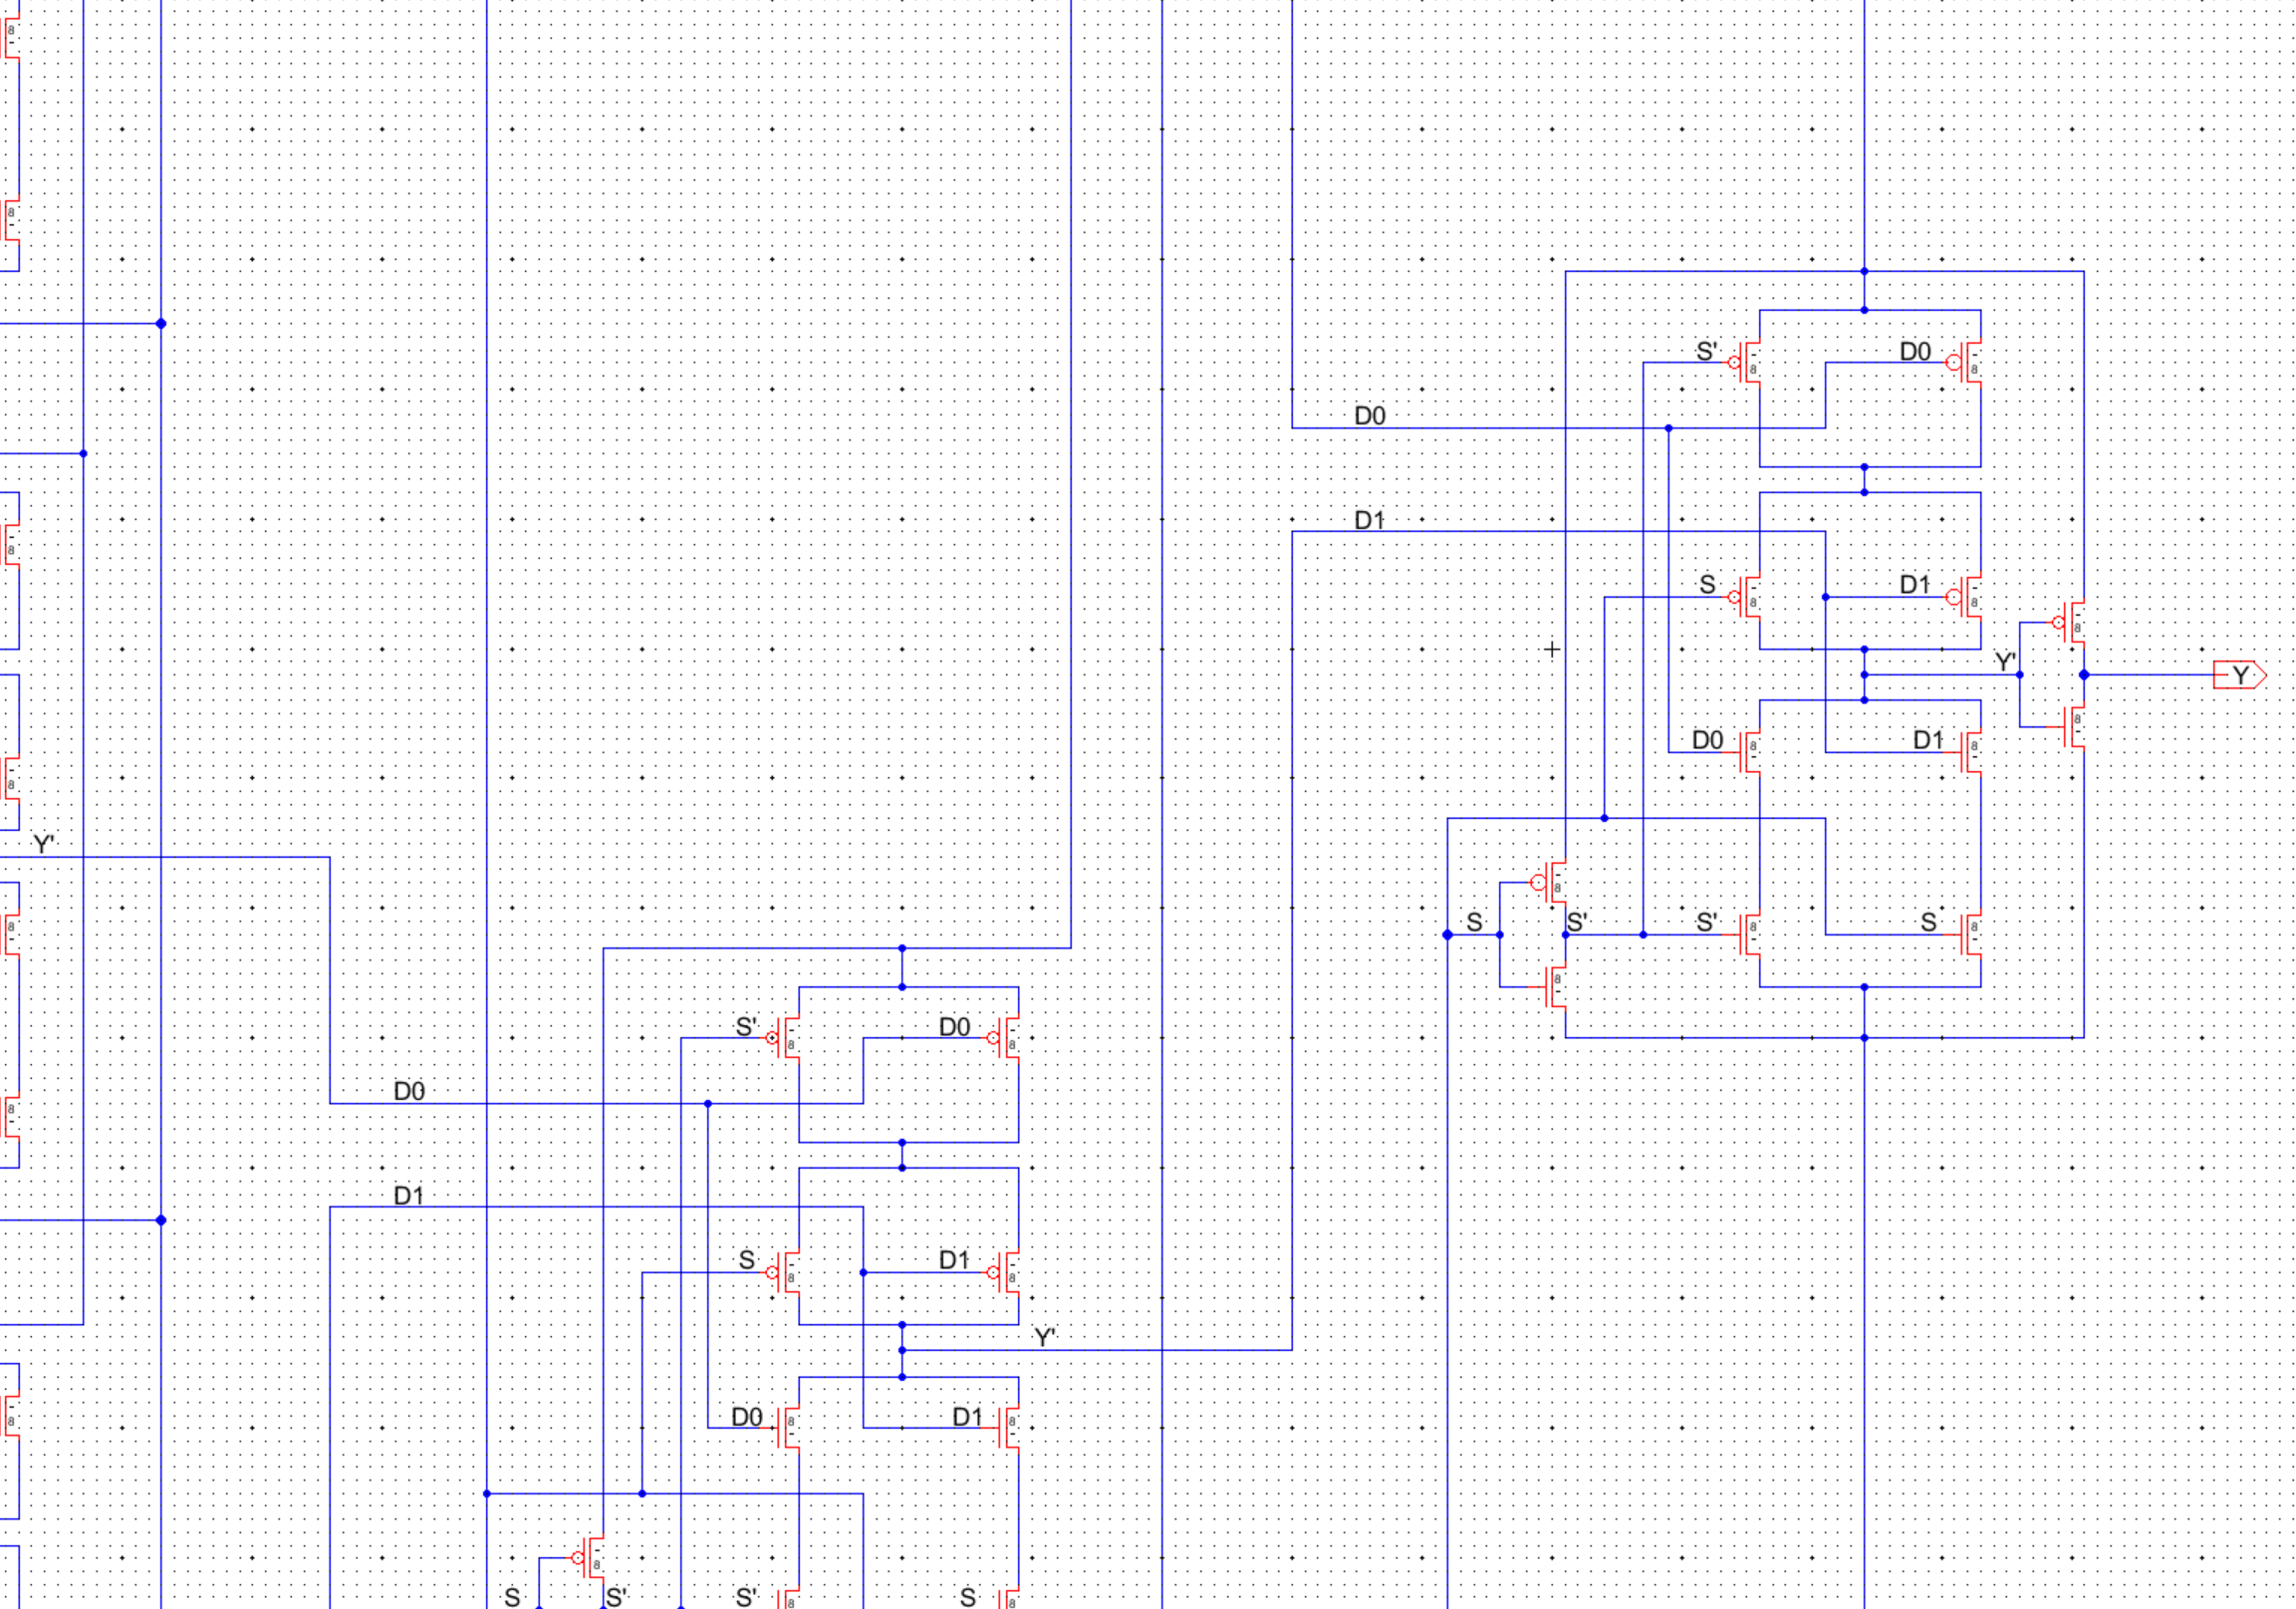
\includegraphics[width=0.9\linewidth, frame]{screenshots/cmos/schem/schem3.png}
      \caption{A close up of the schematic showing the last stage.}
      \label{fig:cmosschem3}
    \end{figure}

    Figure \ref{fig:cmosschemdrc} shows that the schematic passes the DRC check.


    \begin{figure}[H]
      \centering
      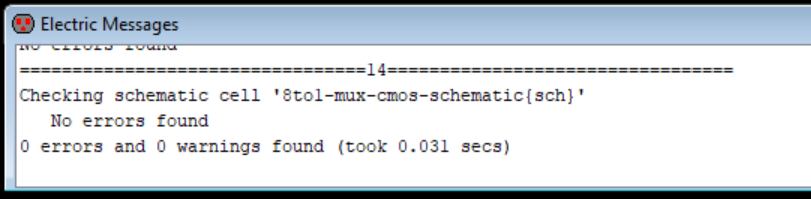
\includegraphics[width=0.6\linewidth, frame]{screenshots/cmos/schem/drc.png}
      \caption{The DRC check for the CMOS schematic.}
      \label{fig:cmosschemdrc}
    \end{figure}


\section{LTSpice Simulation for Schematics}
  \paragraph{}
  This section will detail the LTSpice simulations for both the transmission gate schematic and the CMOS schematic. The spice code used to generate the graphs for this simulation are shown in Figure \ref{fig:simcode}. LTSpice was also used to take measurements that will be detailed later in the report. The code used to generate those measurements is shown in Figure \ref{fig:meascode}.

  \begin{figure}[H]
    \centering
    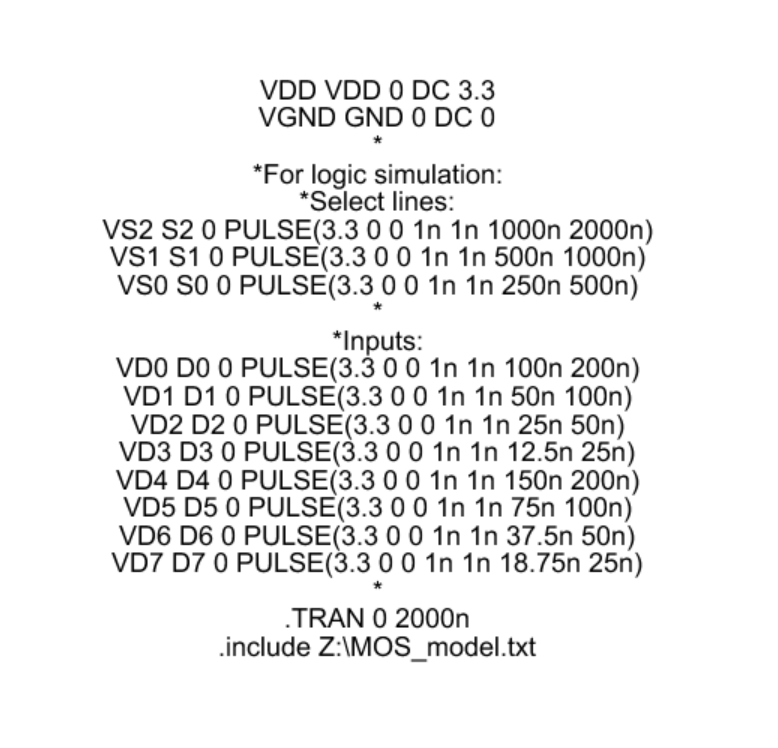
\includegraphics[width=0.5\linewidth, frame]{screenshots/spice-sim-code.png}
    \caption{The LTSpice code used to generate the graphs in the following section.}
    \label{fig:simcode}
  \end{figure}

  \begin{figure}[H]
    \centering
    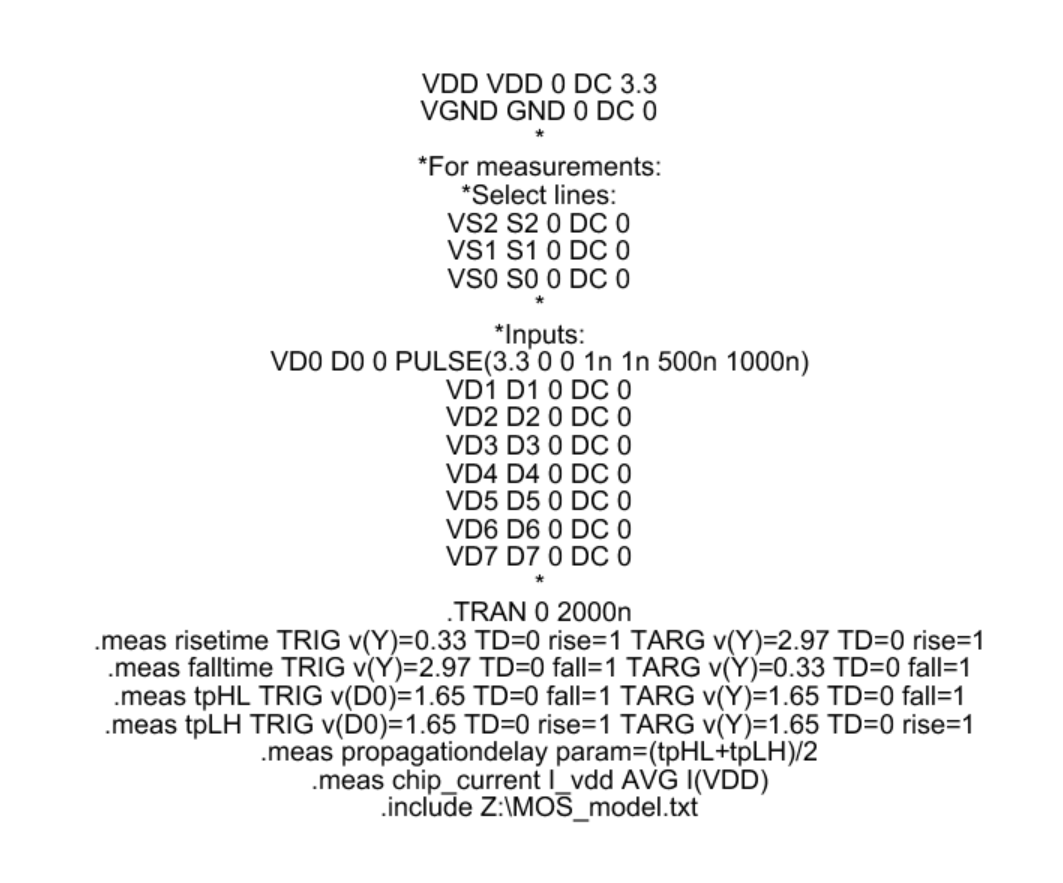
\includegraphics[width=0.5\linewidth, frame]{screenshots/spice-meas-code.png}
    \caption{The LTSpice code used to generate the measurements which will be detailed in a later section.}
    \label{fig:meascode}
  \end{figure}


  \subsection{Transmission Gate Schematic LTSpice}
    \paragraph{}
    The spice simulation for the transmission gate schematic is shown in Figure \ref{fig:tgspice}. The inputs D0 through D7 are shown first, each with their own uniquely identifying waveform. The select line is stepped through all eight values from 000 to 111, each corresponding to the inputs D0 through D7 as shown in the figure. At the output Y, the correct waveform can be seen corresponding to the selected input. The waveforms have been highlighted with a colored dotted rectangle to show the location of the input and the output at Y. This figure illustrates the expected behavior.

    \begin{figure}[H]
      \centering
      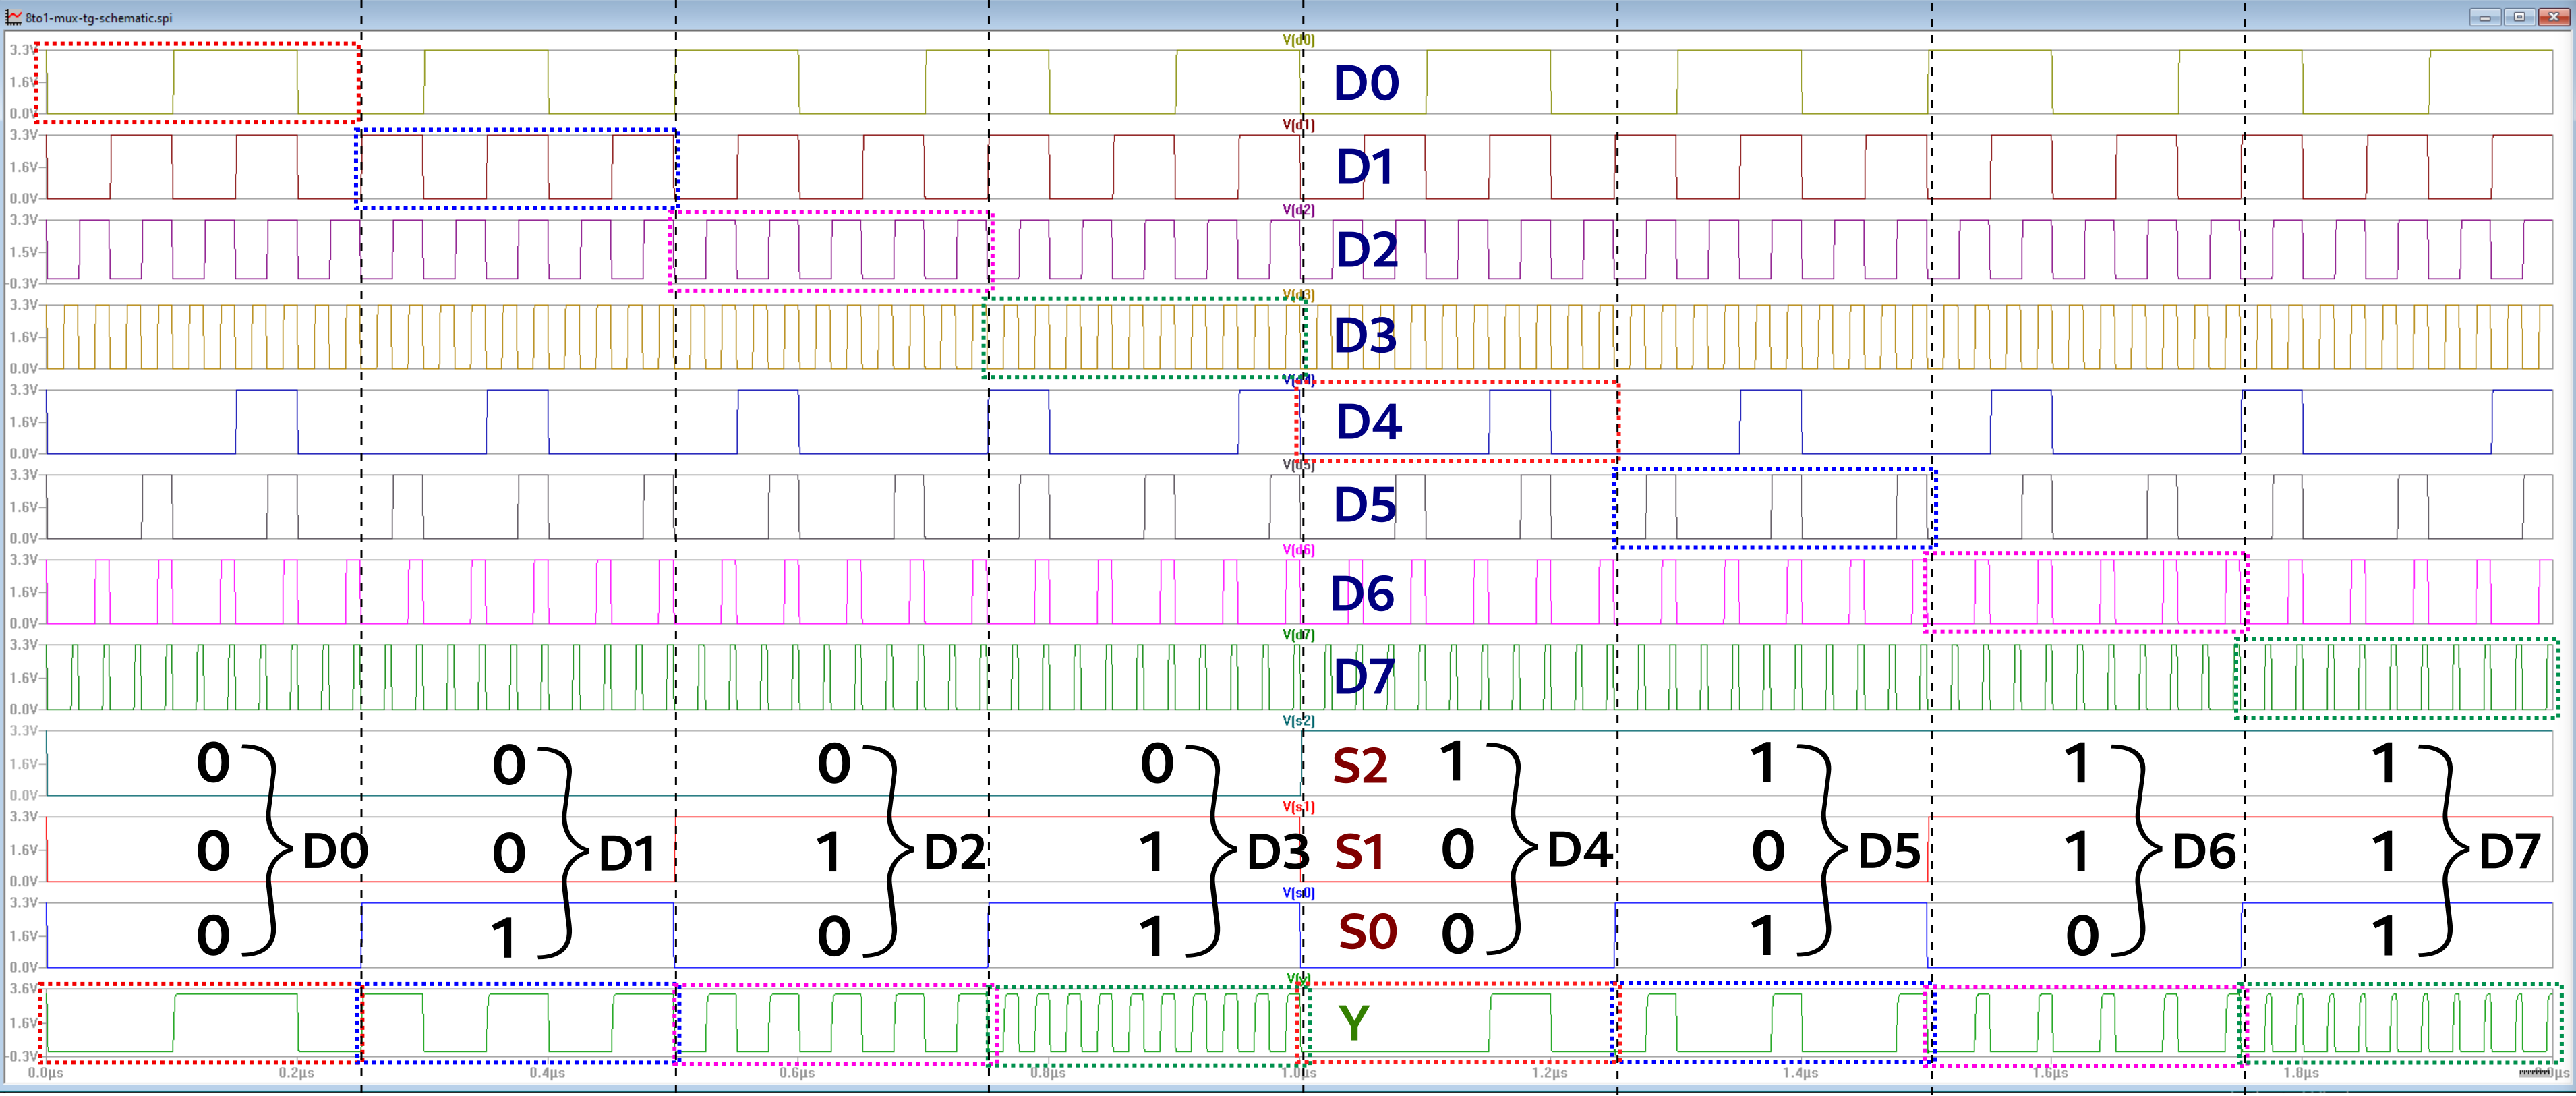
\includegraphics[width=\linewidth, frame]{screenshots/tg/schem/spice.png}
      \caption{The LTSpice simulation of the transmission gate schematic showing that each combination of inputs to the select line passes through the corresponding inputs D0 through D7.}
      \label{fig:tgspice}
    \end{figure}

    \paragraph{}
    The measurements obtained with the spice code shown in Figure \ref{fig:meascode} for the transmission gate schematic are shown in Figure \ref{fig:tgschemmeas}.

    \begin{figure}[H]
      \centering
      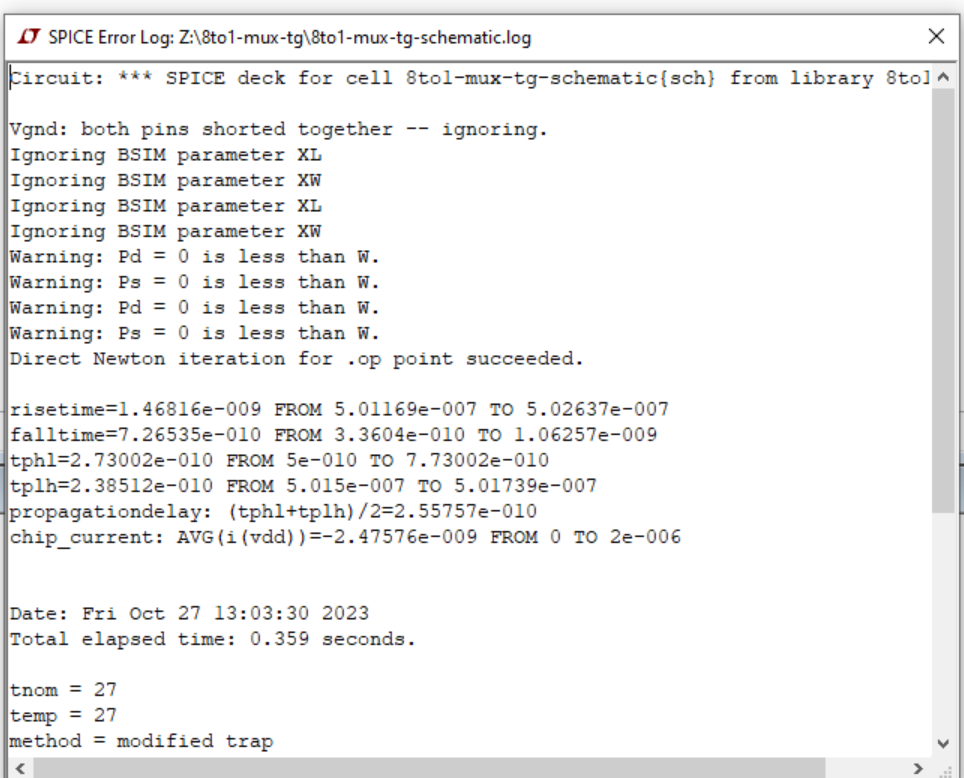
\includegraphics[width=0.5\linewidth, frame]{screenshots/tg/schem/meas.png}
      \caption{The measurements obtained through LTSpice simulation of the transmission gate schematic.}
      \label{fig:tgschemmeas}
    \end{figure}



  \subsection{CMOS Schematic LTSpice}
    \paragraph{}
    The spice simulation for the CMOS schematic is shown in Figure \ref{fig:cmosspice}. As described in the last subsection, the behavior in the graph is as expected. Each input is passed through to the output when selected by the select line.


    \begin{figure}[H]
      \centering
      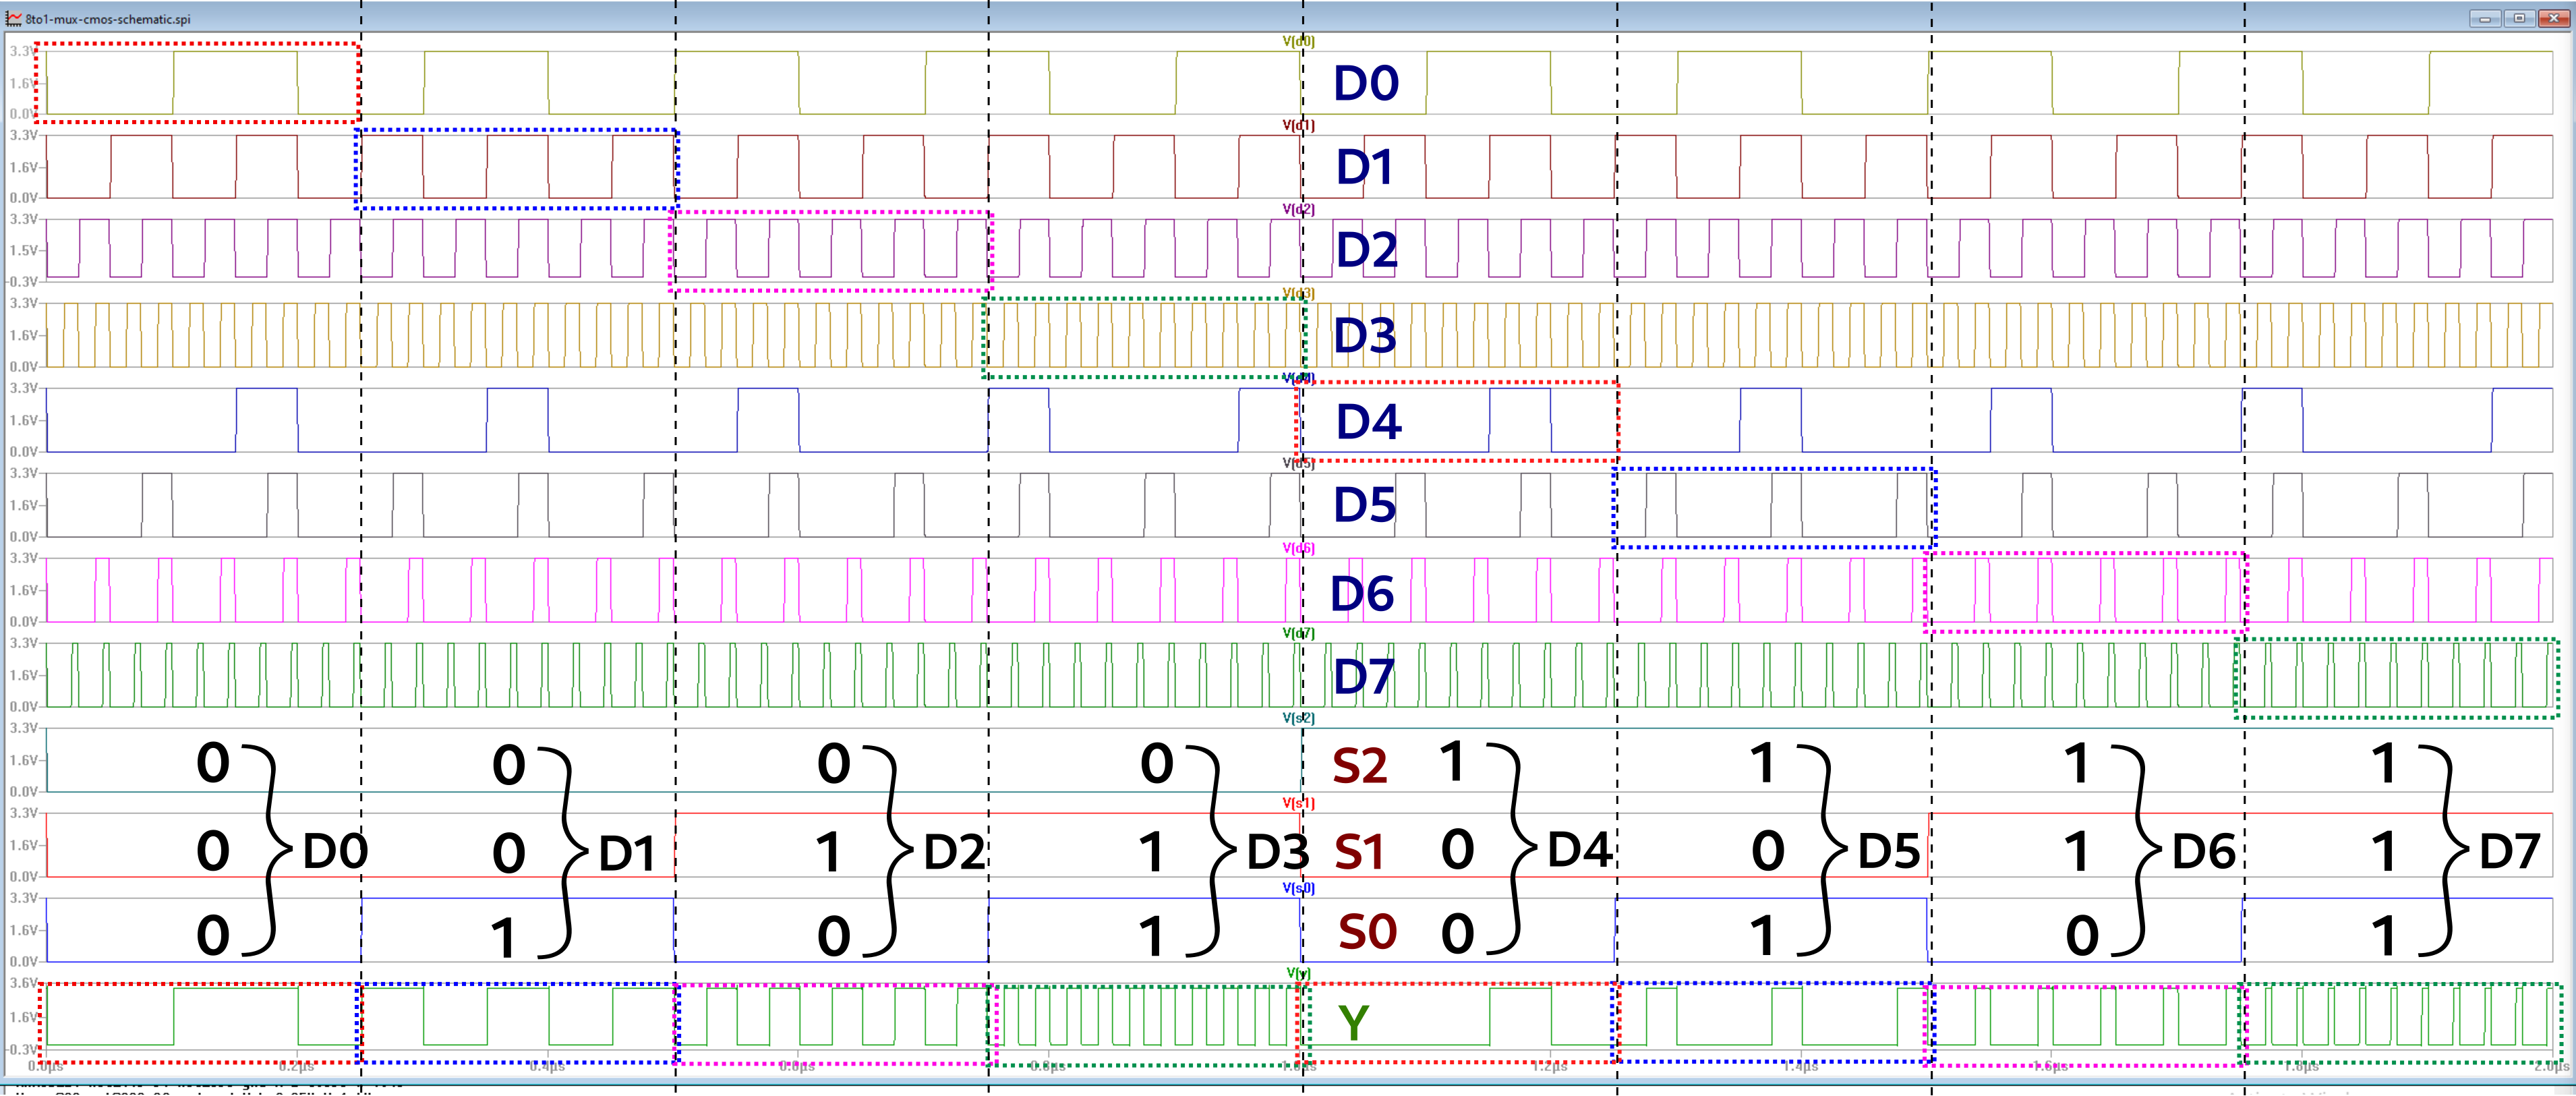
\includegraphics[width=\linewidth, frame]{screenshots/cmos/schem/spice.png}
      \caption{The LTSpice simulation of the CMOS schematic showing that each combination of inputs to the select line passes through the corresponding inputs D0 through D7.}
      \label{fig:cmosspice}
    \end{figure}


    \paragraph{}
    The measurements obtained with the spice code shown in Figure \ref{fig:meascode} for the CMOS schematic are shown in Figure \ref{fig:cmosschemmeas}.

    \begin{figure}[H]
      \centering
      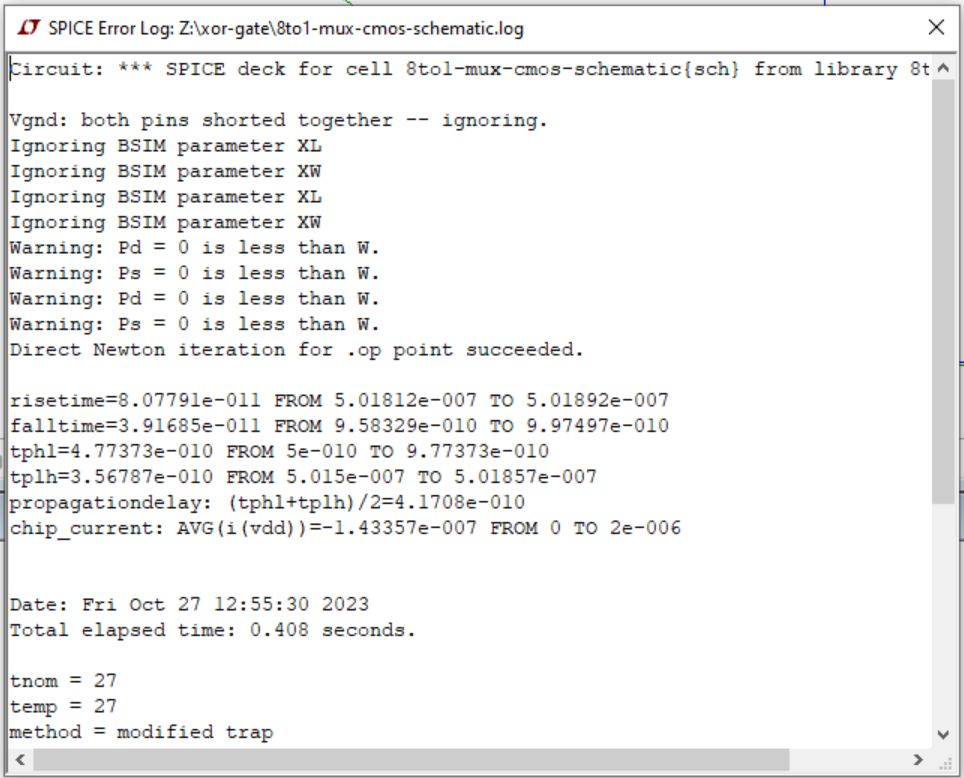
\includegraphics[width=0.5\linewidth, frame]{screenshots/cmos/schem/meas.png}
      \caption{The measurements obtained through LTSpice simulation of the CMOS schematic.}
      \label{fig:cmosschemmeas}
    \end{figure}



\section{IRSIM for Schematic}
  \paragraph{}
  This section details the IRSIM simulations done on both the transmission gate schematic and the CMOS schematic. I chose to simulate only one D input per screenshot and two per design. This is because IRSIM can be buggy and has a hard time with too many inputs changing at once.  

  \subsection{Transmission Gate Schematic IRSIM}
    \paragraph{}
    The IRSIM simulation for the transmission gate schematic is shown in Figure \ref{fig:tgschemirsim1} and \ref{fig:tgschemirsim2}. As shown in the screenshots, the schematic behaves as expected.

    \begin{figure}[H]
      \centering
      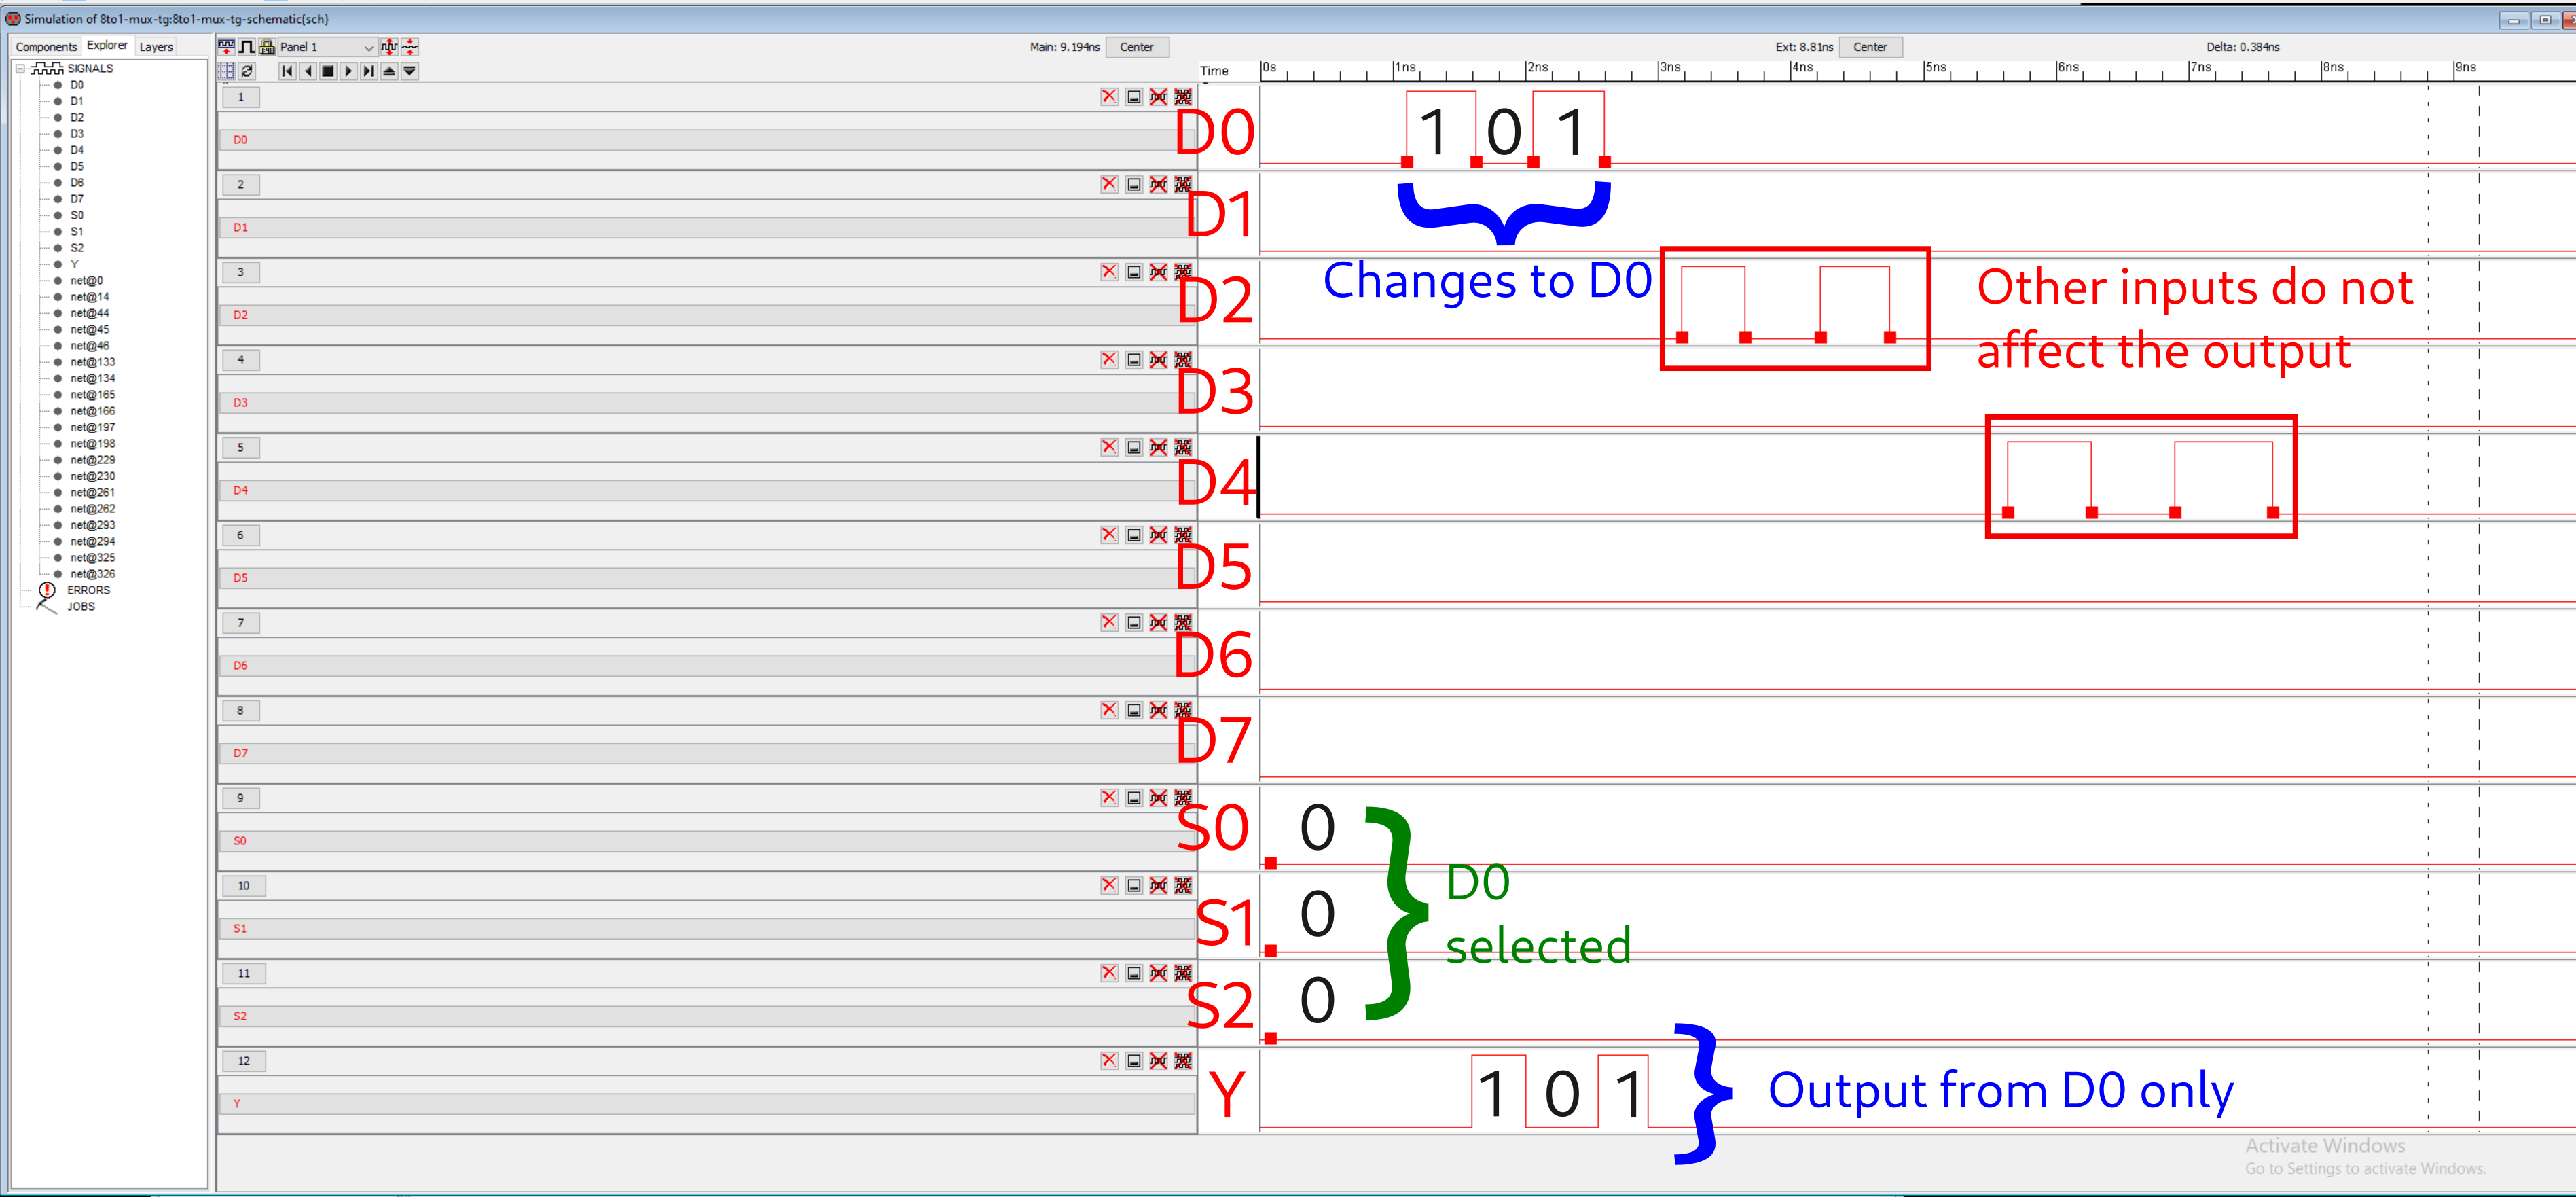
\includegraphics[width=\linewidth, frame]{screenshots/tg/schem/irsim.png}
      \caption{One IRSIM simulation for the transmission gate schematic showing that the design works as expected.}
      \label{fig:tgschemirsim1}
    \end{figure}


    \begin{figure}[H]
      \centering
      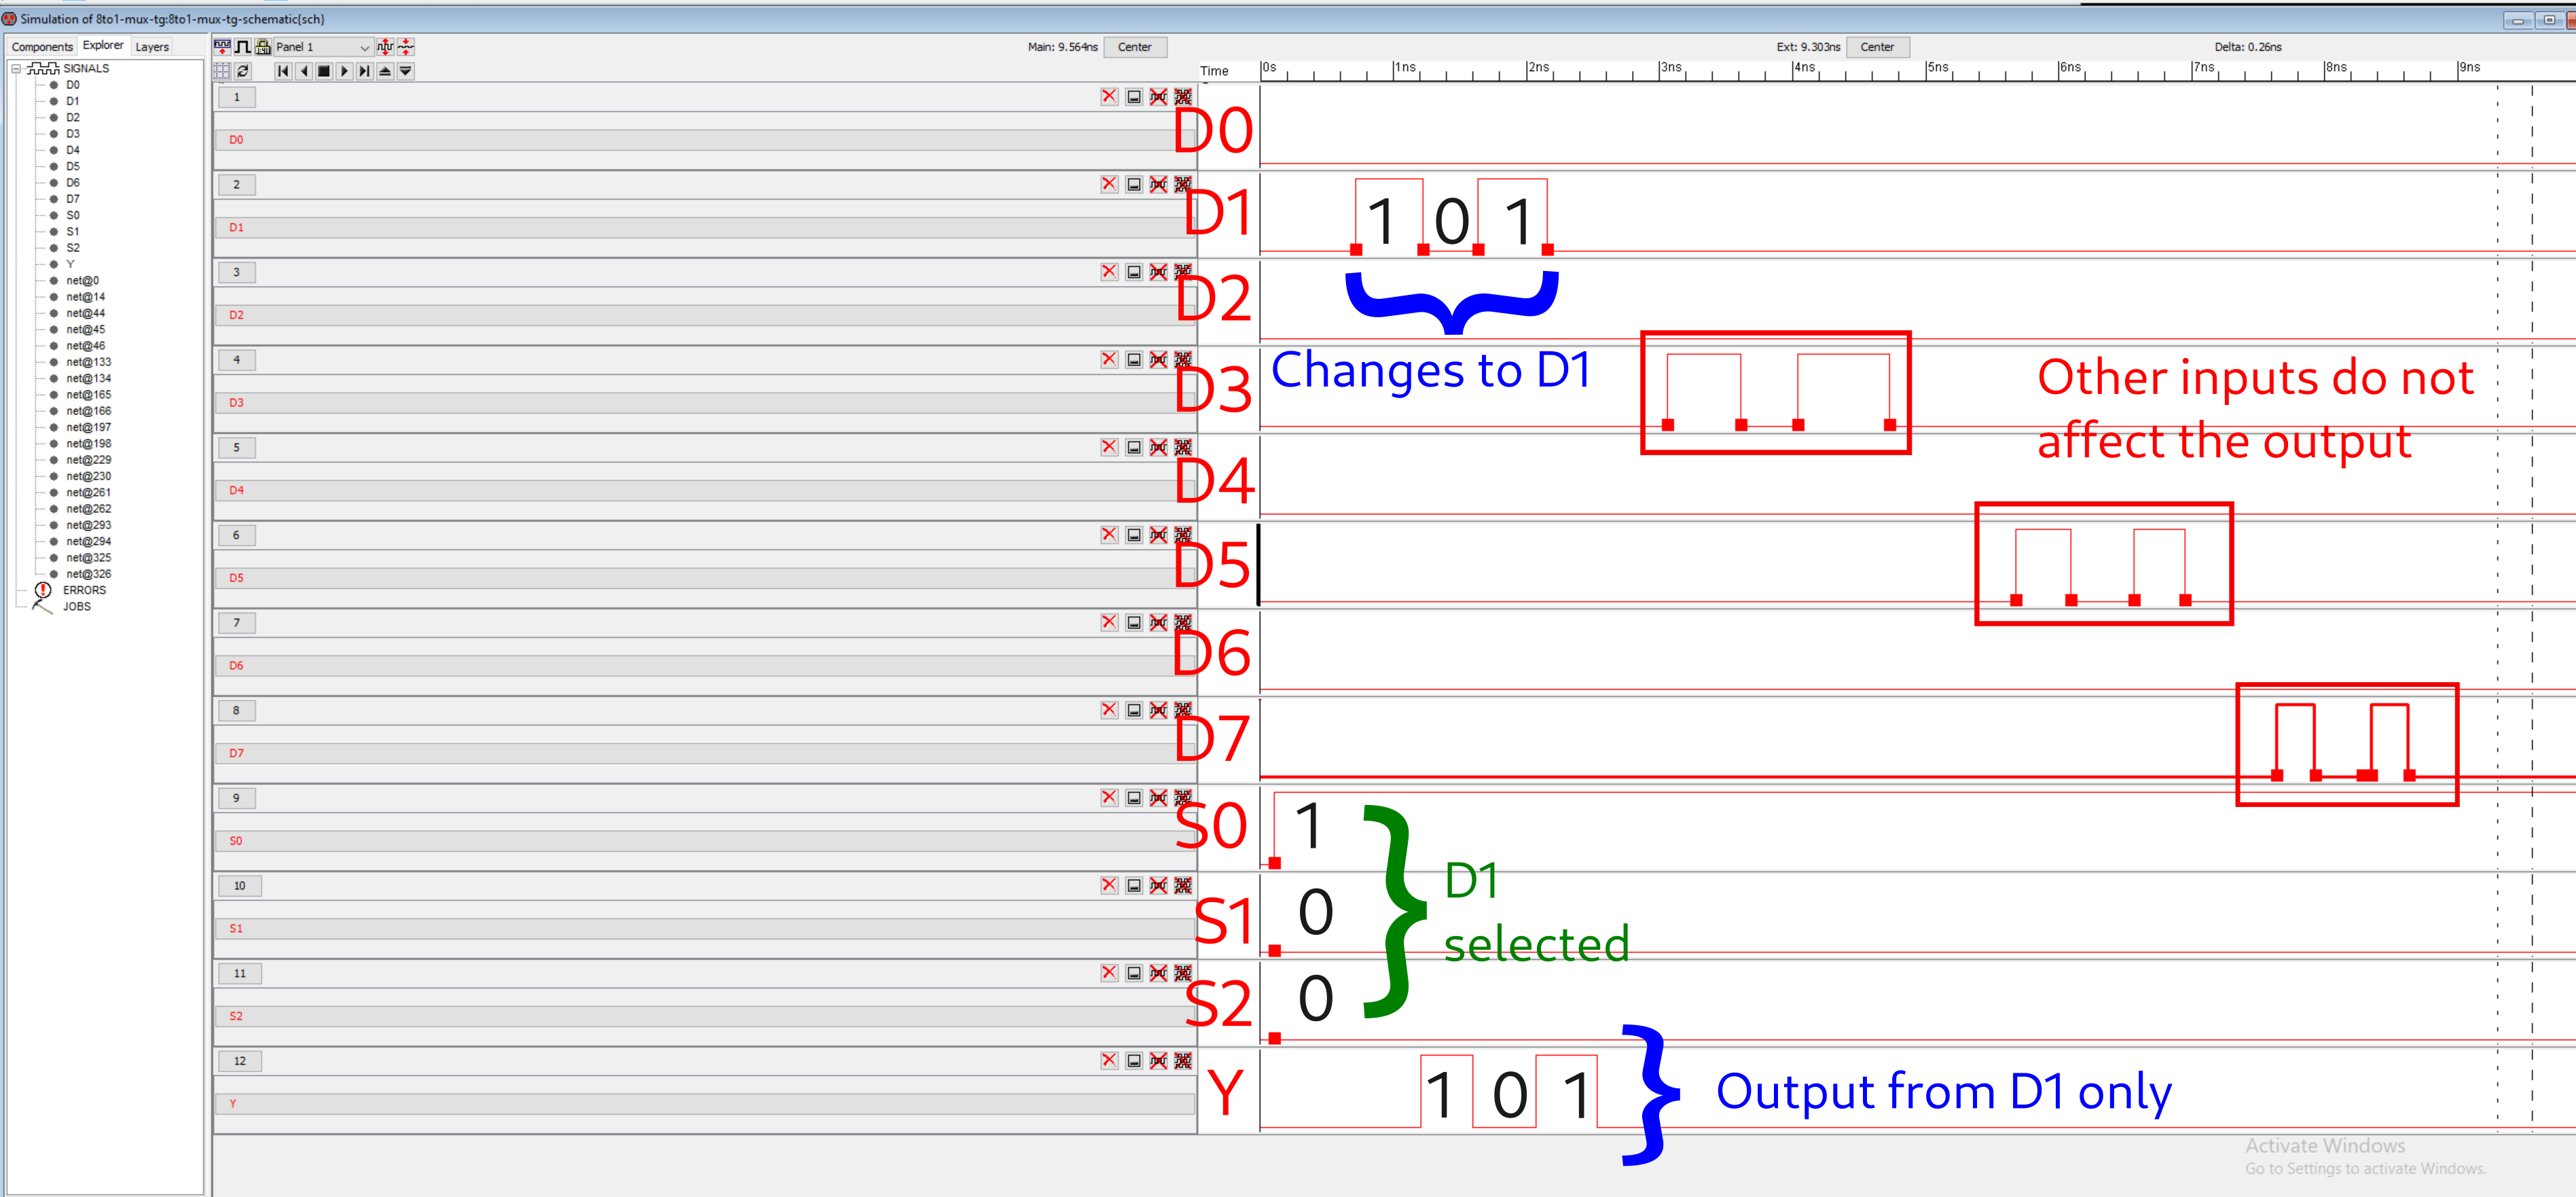
\includegraphics[width=\linewidth, frame]{screenshots/tg/schem/irsim2.png}
      \caption{Another IRSIM simulation for the transmission gate schematic showing that the design works as expected.}
      \label{fig:tgschemirsim2}
    \end{figure}


  \subsection{CMOS Schematic IRSIM}
    \paragraph{}
    The IRSIM simulation for the CMOS schematic is shown in Figure \ref{fig:cmosschemirsim1} and \ref{fig:cmosschemirsim2}. As shown in the screenshots, the schematic behaves as expected.

    \begin{figure}[H]
      \centering
      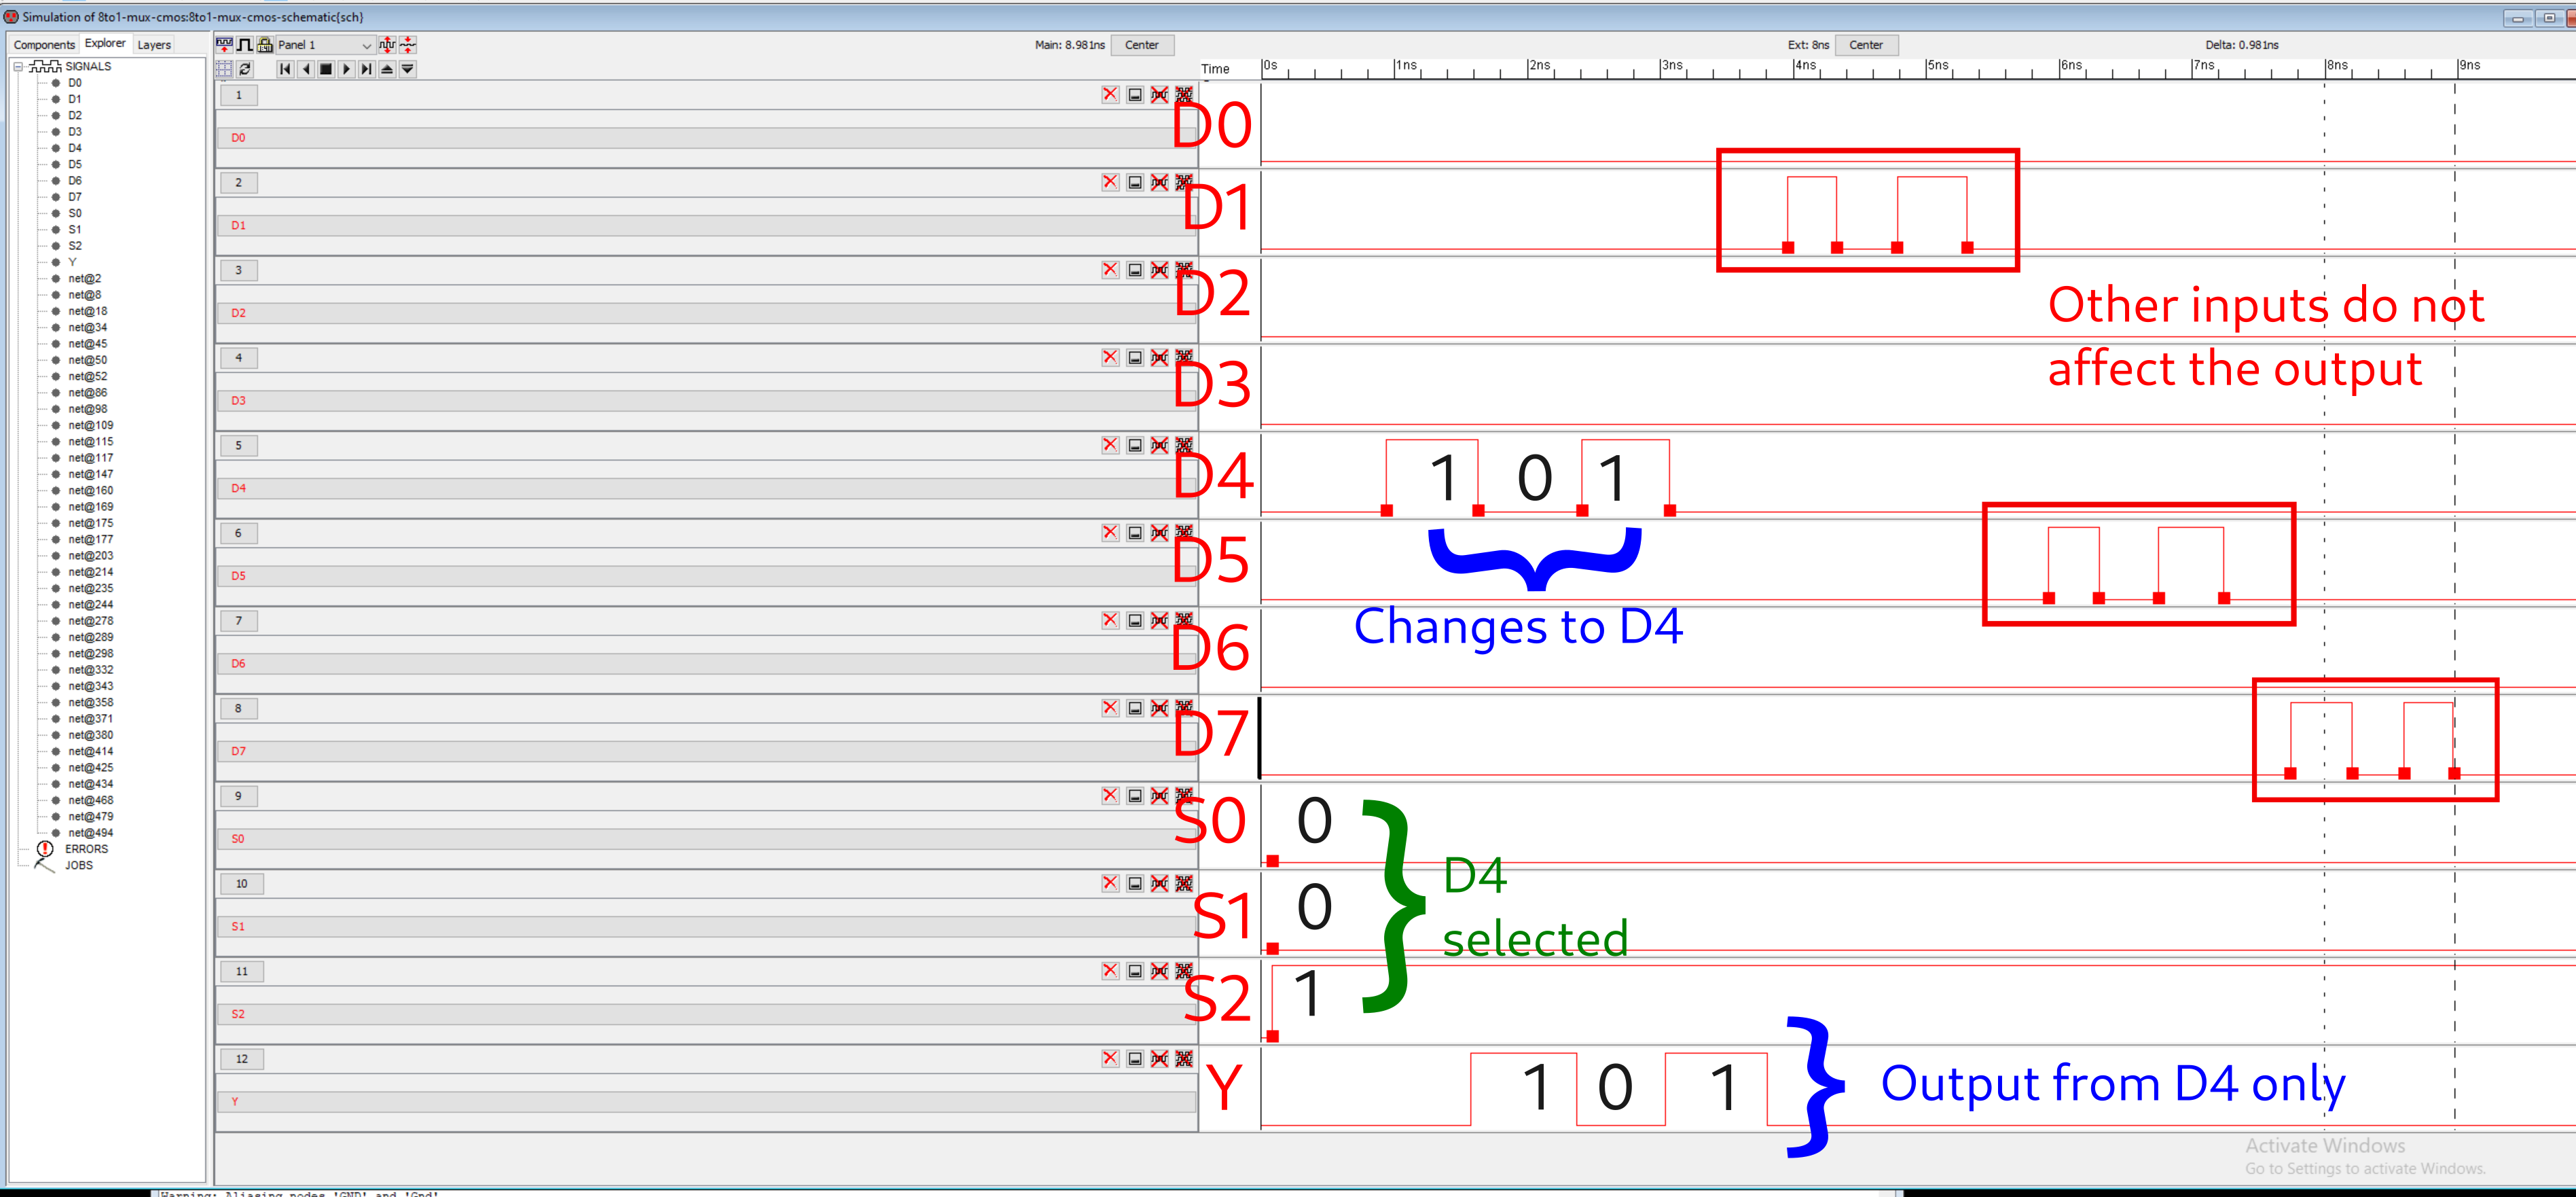
\includegraphics[width=\linewidth, frame]{screenshots/cmos/schem/irsim.png}
      \caption{One IRSIM simulation for the CMOS schematic showing that the design works as expected.}
      \label{fig:cmosschemirsim1}
    \end{figure}


    \begin{figure}[H]
      \centering
      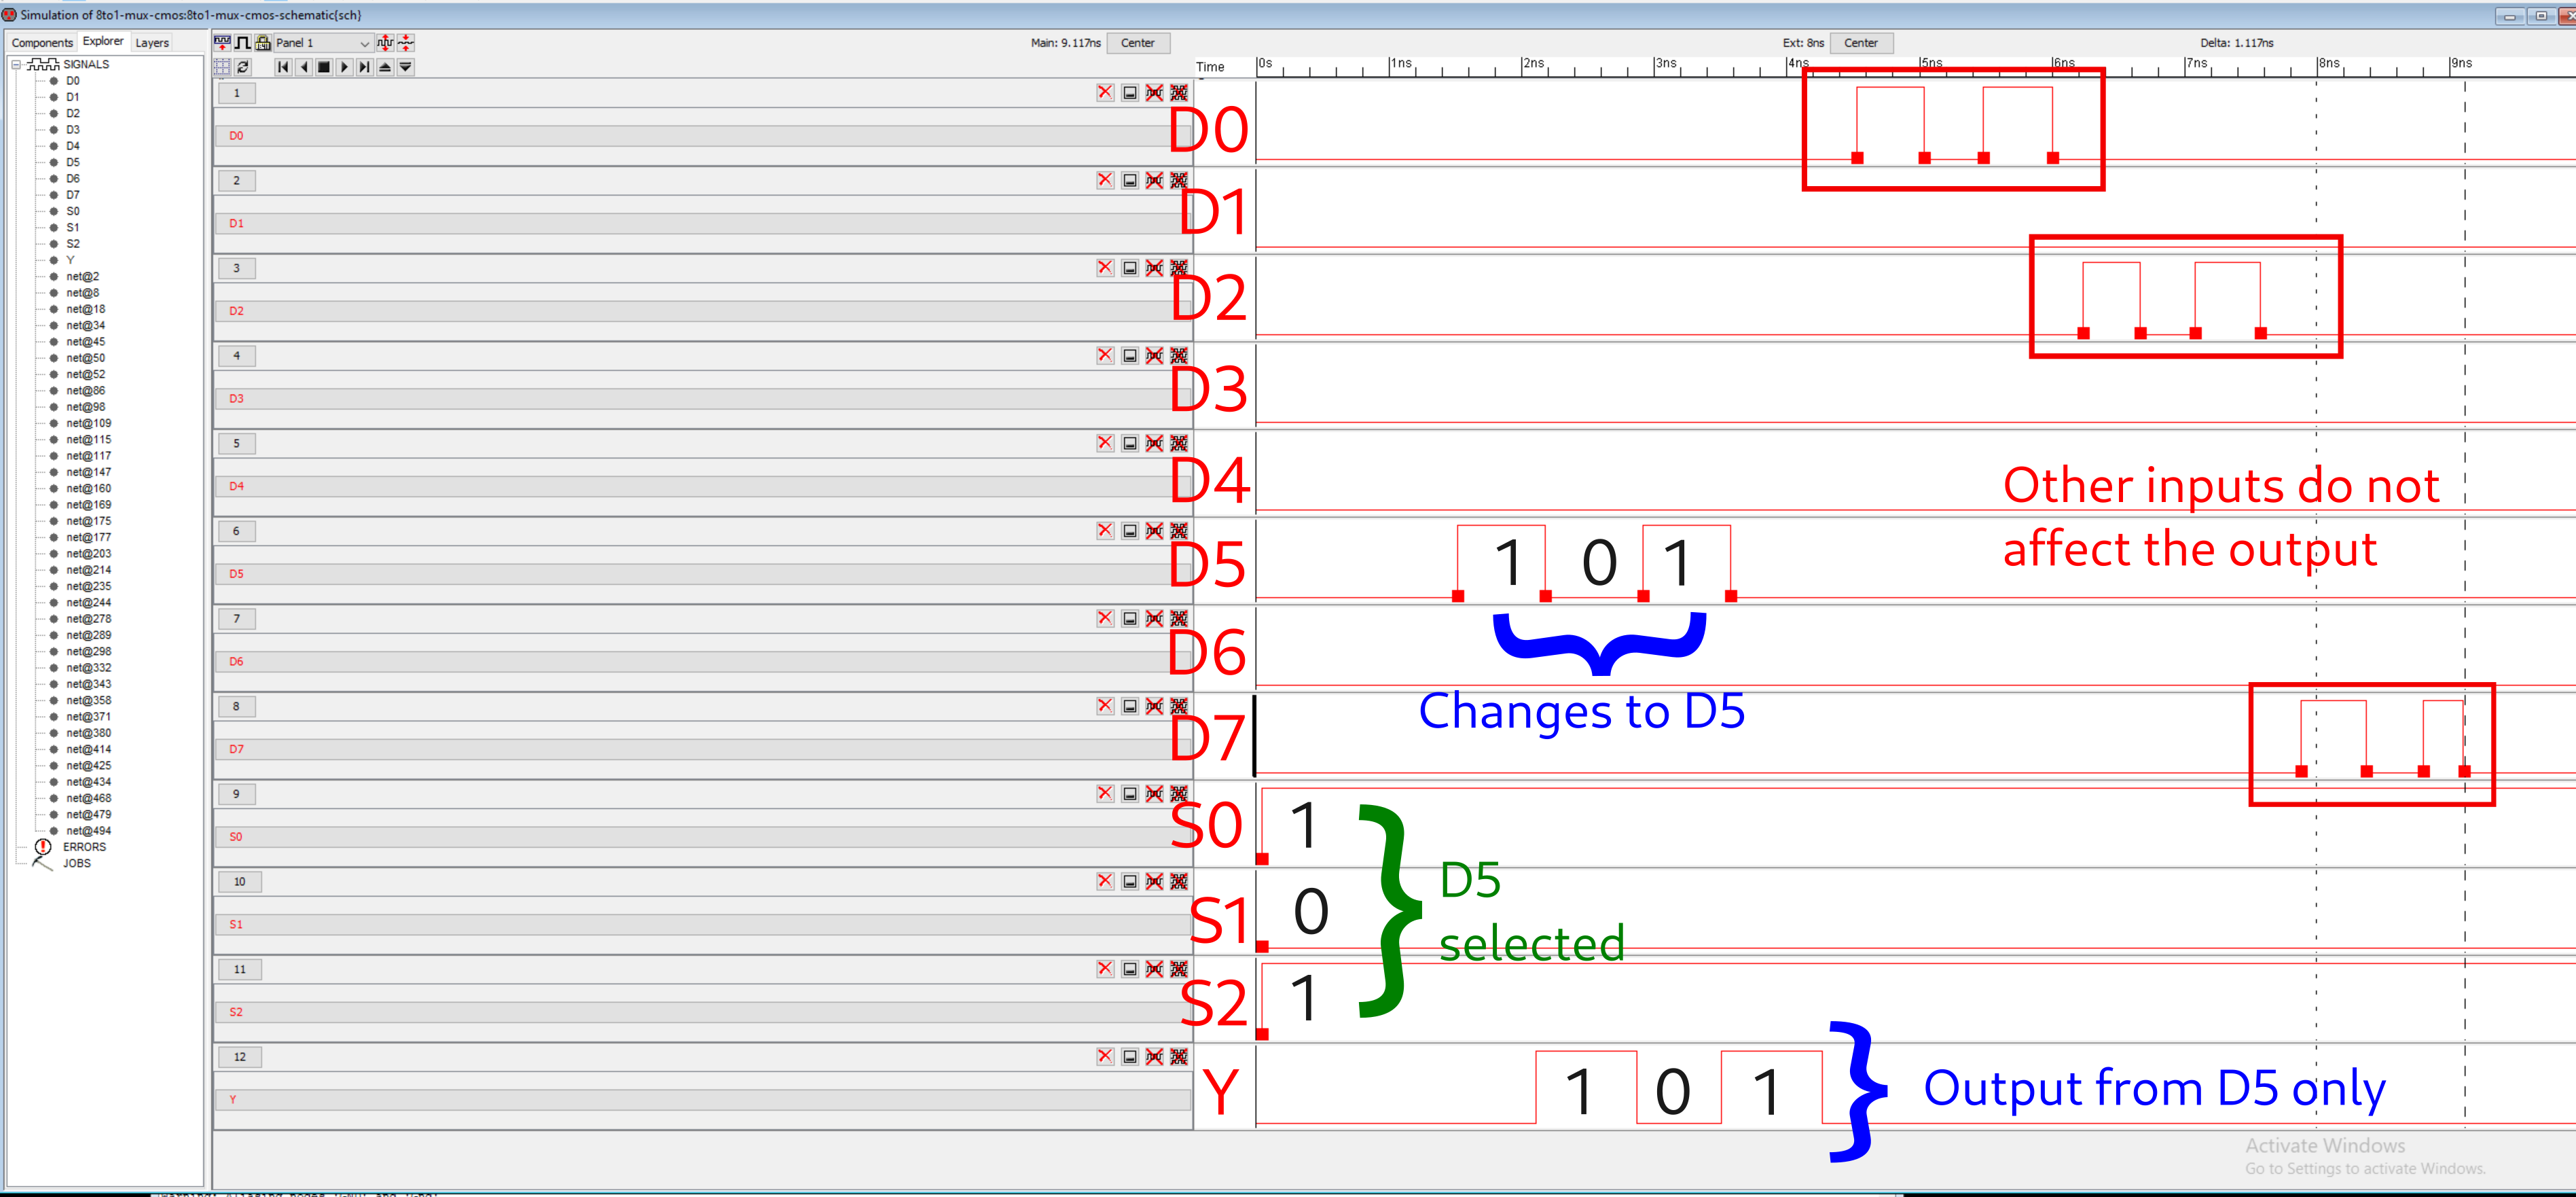
\includegraphics[width=\linewidth, frame]{screenshots/cmos/schem/irsim2.png}
      \caption{Another IRSIM simulation for the CMOS schematic showing that the design works as expected.}
      \label{fig:cmosschemirsim2}
    \end{figure}

\section{Electric Layouts}
  \paragraph{}
  This section details the design of the layouts in Electric for both the transmission gate multiplexer and the CMOS multiplexer.

  \subsection{Transmission Gate Layout}
    \paragraph{}
    The transmission gate layout of the 8-to-1 multiplexer is shown in Figure \ref{fig:tglay1}. I first designed one set of three transmission gates and then stacked them, running the inputs to the sets along the left and right. I had to pay careful attention to the layout of each set of gates to make sure that I could run the proper signals to each. A close up of the individual sets of transmission gates is shown in Figure \ref{fig:tglay2}. I placed the inverters for the select line at the bottom as shown in Figure \ref{fig:tglay3}. On the left of the transmission gates are metal and polysilicon lines for $S_2$, $\overline{S_2}$, and $S_1$, and to the right are lines for $\overline{S_1}$, $\overline{S_0}$, and $S_0$. I also had to route VDD to the right as well.


    \begin{figure}[H]
      \centering
      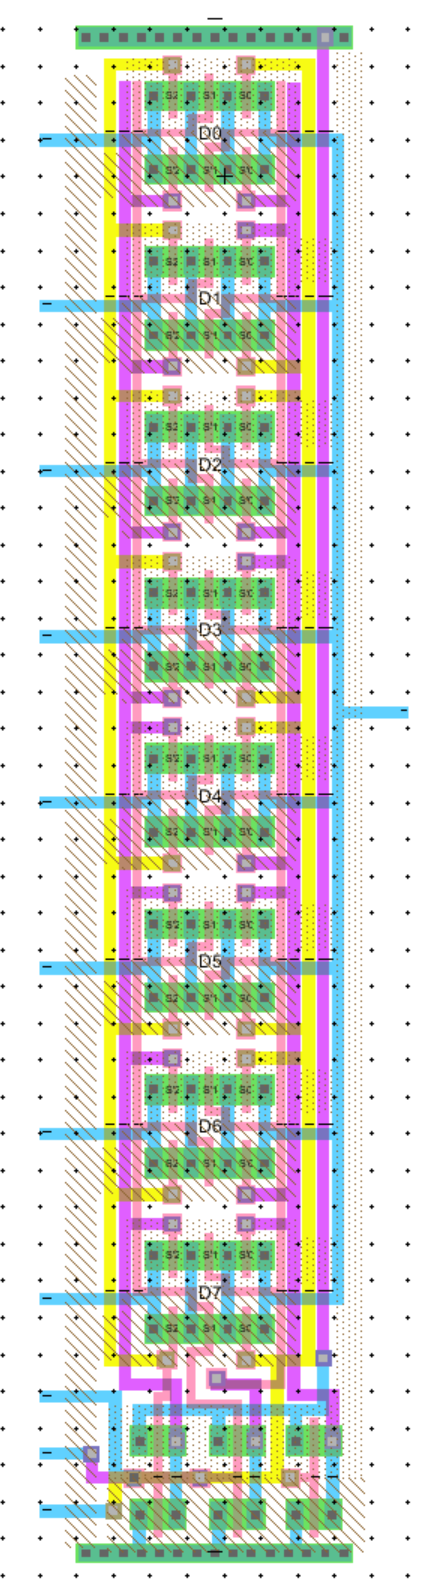
\includegraphics[width=0.4\linewidth, frame]{screenshots/tg/lay/lay1.png}
      \caption{The layout for the transmission gate design of the 8-to-1 multiplexer.}
      \label{fig:tglay1}
    \end{figure}


    \begin{figure}[H]
      \centering
      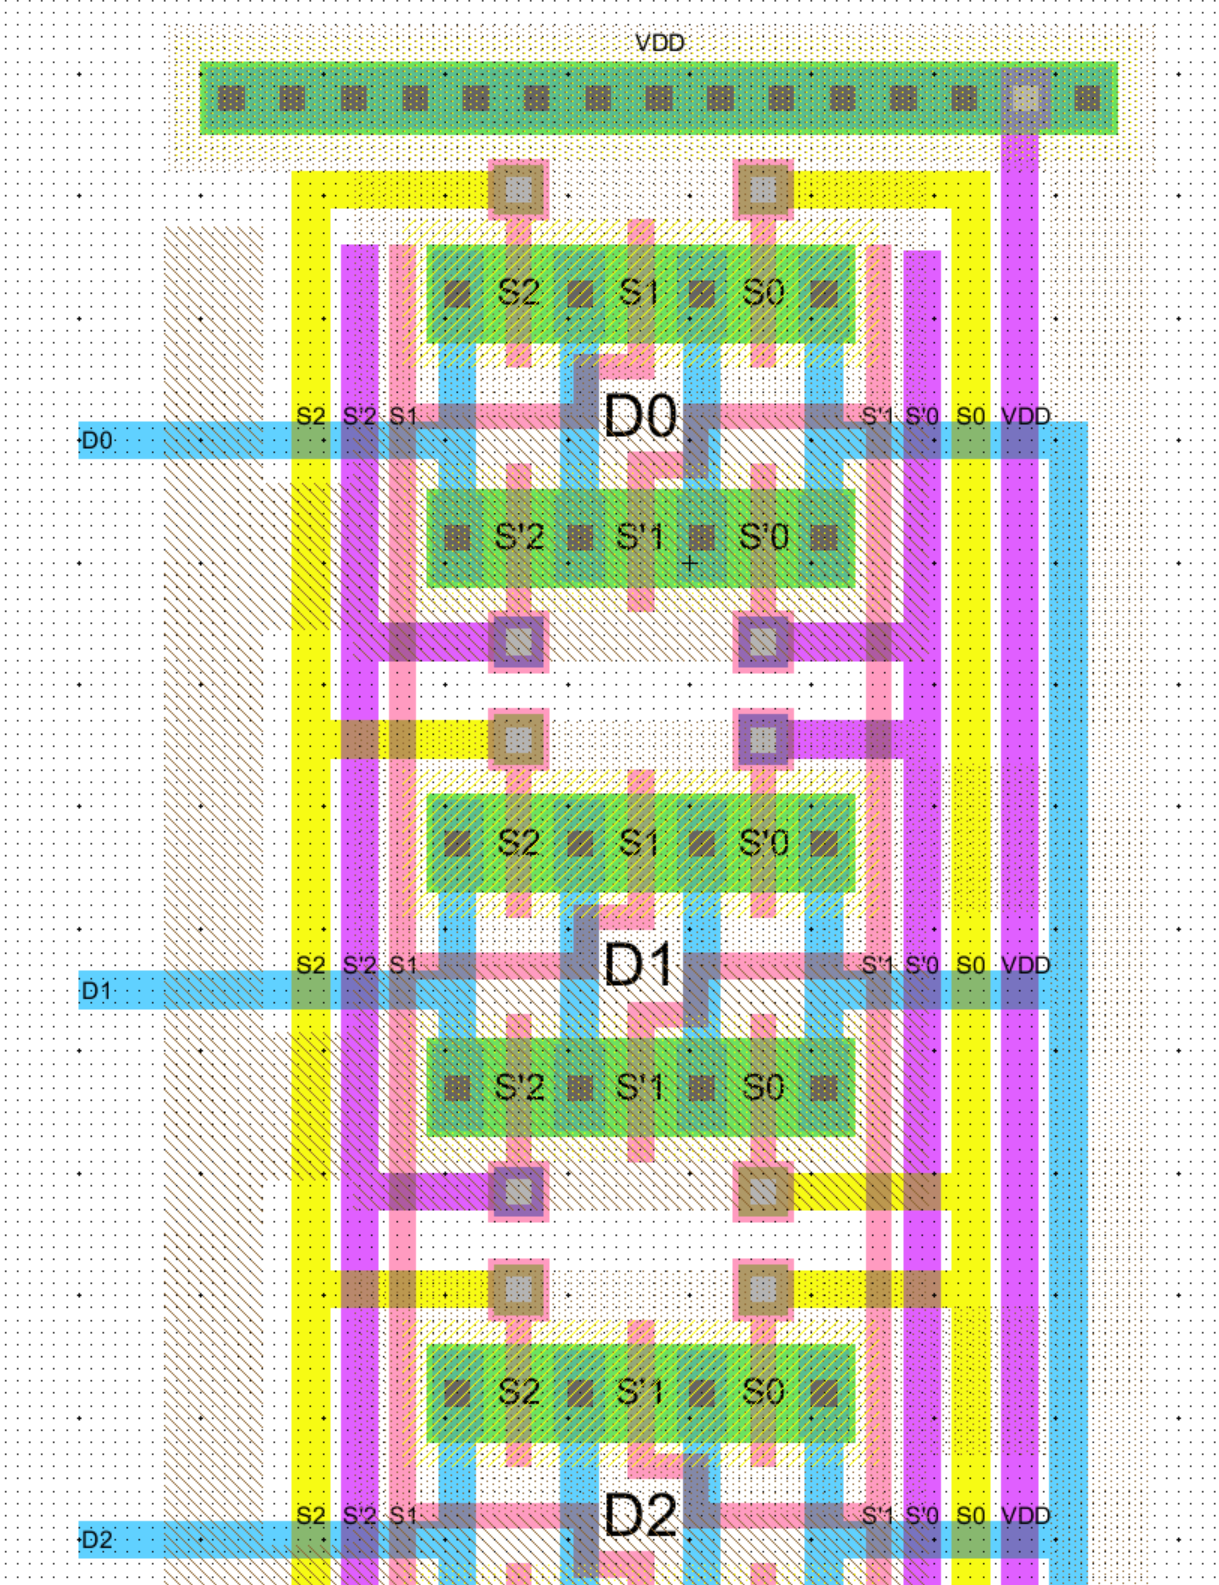
\includegraphics[width=0.45\linewidth, frame]{screenshots/tg/lay/lay2.png}
      \caption{A close up of the sets of transmission gates for the layout.}
      \label{fig:tglay2}
    \end{figure}

    \begin{figure}[H]
      \centering
      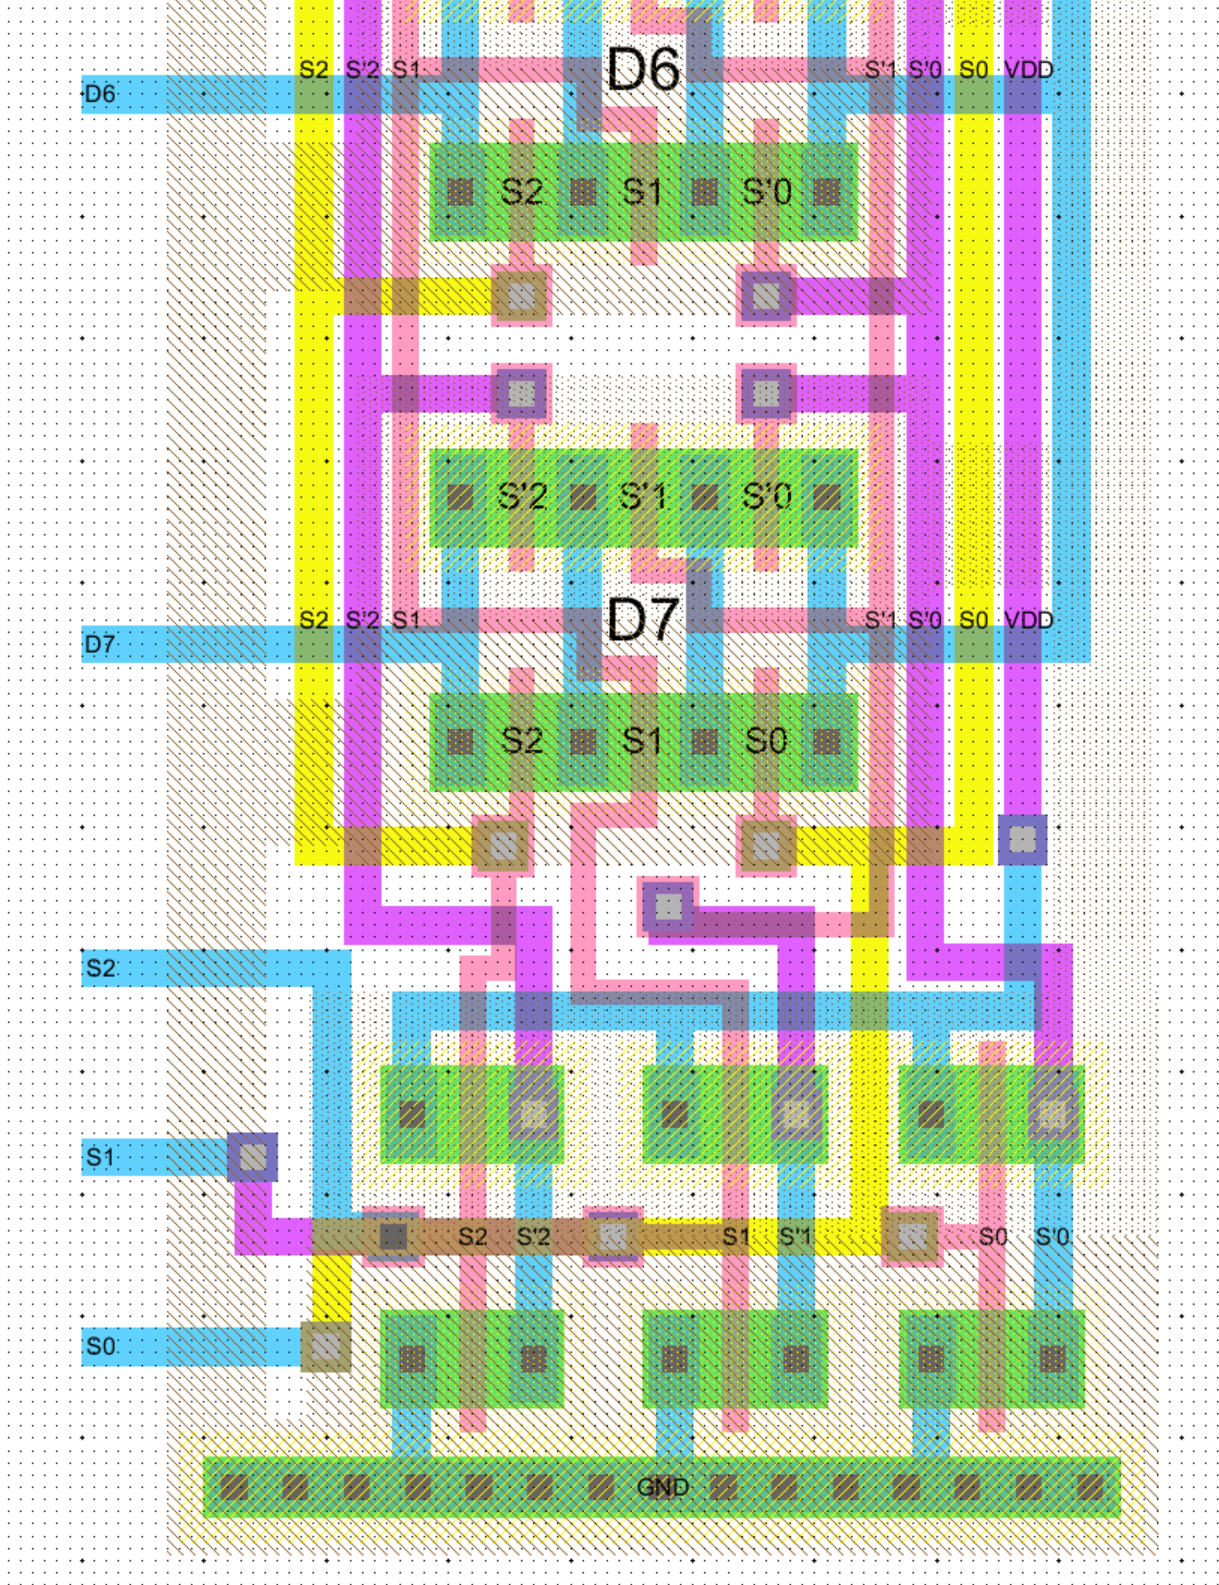
\includegraphics[width=0.45\linewidth, frame]{screenshots/tg/lay/lay3.png}
      \caption{A close up of the inverters at the bottom of the transmission gate layout.}
      \label{fig:tglay3}
    \end{figure}

    \paragraph{}
    The DRC results are shown in Figure \ref{fig:tglaydrc} and the well check results are shown in Figure \ref{fig:tglaywell}, both showing no errors.

    \begin{figure}[H]
      \centering
      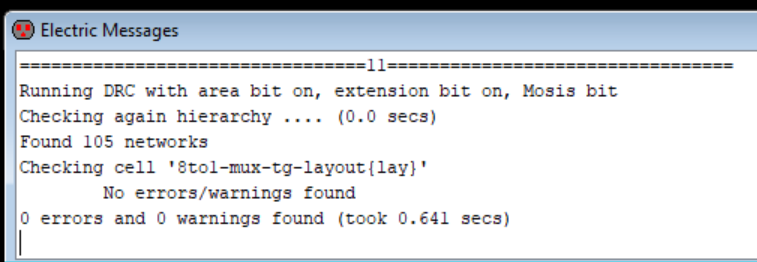
\includegraphics[width=0.6\linewidth, frame]{screenshots/tg/lay/drc.png}
      \caption{The DRC results for the transmission gate layout showing no errors.}
      \label{fig:tglaydrc}
    \end{figure}


    \begin{figure}[H]
      \centering
      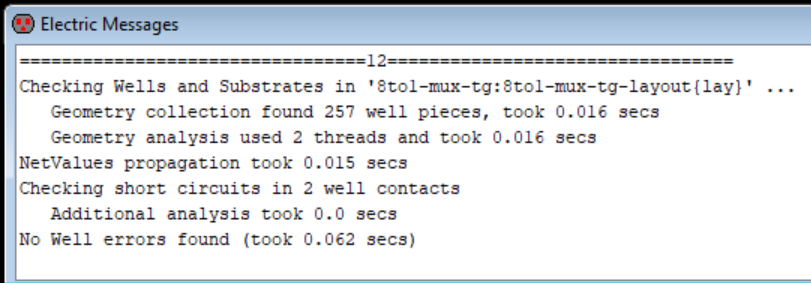
\includegraphics[width=0.6\linewidth, frame]{screenshots/tg/lay/well.png}
      \caption{The well check results for the transmission gate layout showing no errors.}
      \label{fig:tglaywell}
    \end{figure}



  \subsection{CMOS Layout}
    \paragraph{}
    The CMOS layout of the 8-to-1 multiplexer is shown in Figure \ref{fig:cmoslay1}. I first designed one 2-to-1 inverter based off of the stick diagram shown in Figure \ref{fig:stick}. I then planned out how I would arrange the seven 2-to-1 multiplexers. I decided the most space-efficient approach would be to make the cell two multiplexers high. The first four multiplexers take all 8 of the inputs. I used metal 2 and metal 3 to bring the inputs over the multiplexers to their inputs. I then connected the output of those four multiplexers to another two multiplexers, and then the output of those two to another singular multiplexer. I then managed to fit the inverter above the final multiplexer. I ran the select lines at the bottom of the design. Figure \ref{fig:cmoslay2} shows a close up of the first stage, consisting of four 2-to-1 multiplexers. Figure \ref{fig:cmoslay3} shows a close up of the last two stages and the inverter.

    \begin{figure}[H]
      \centering
      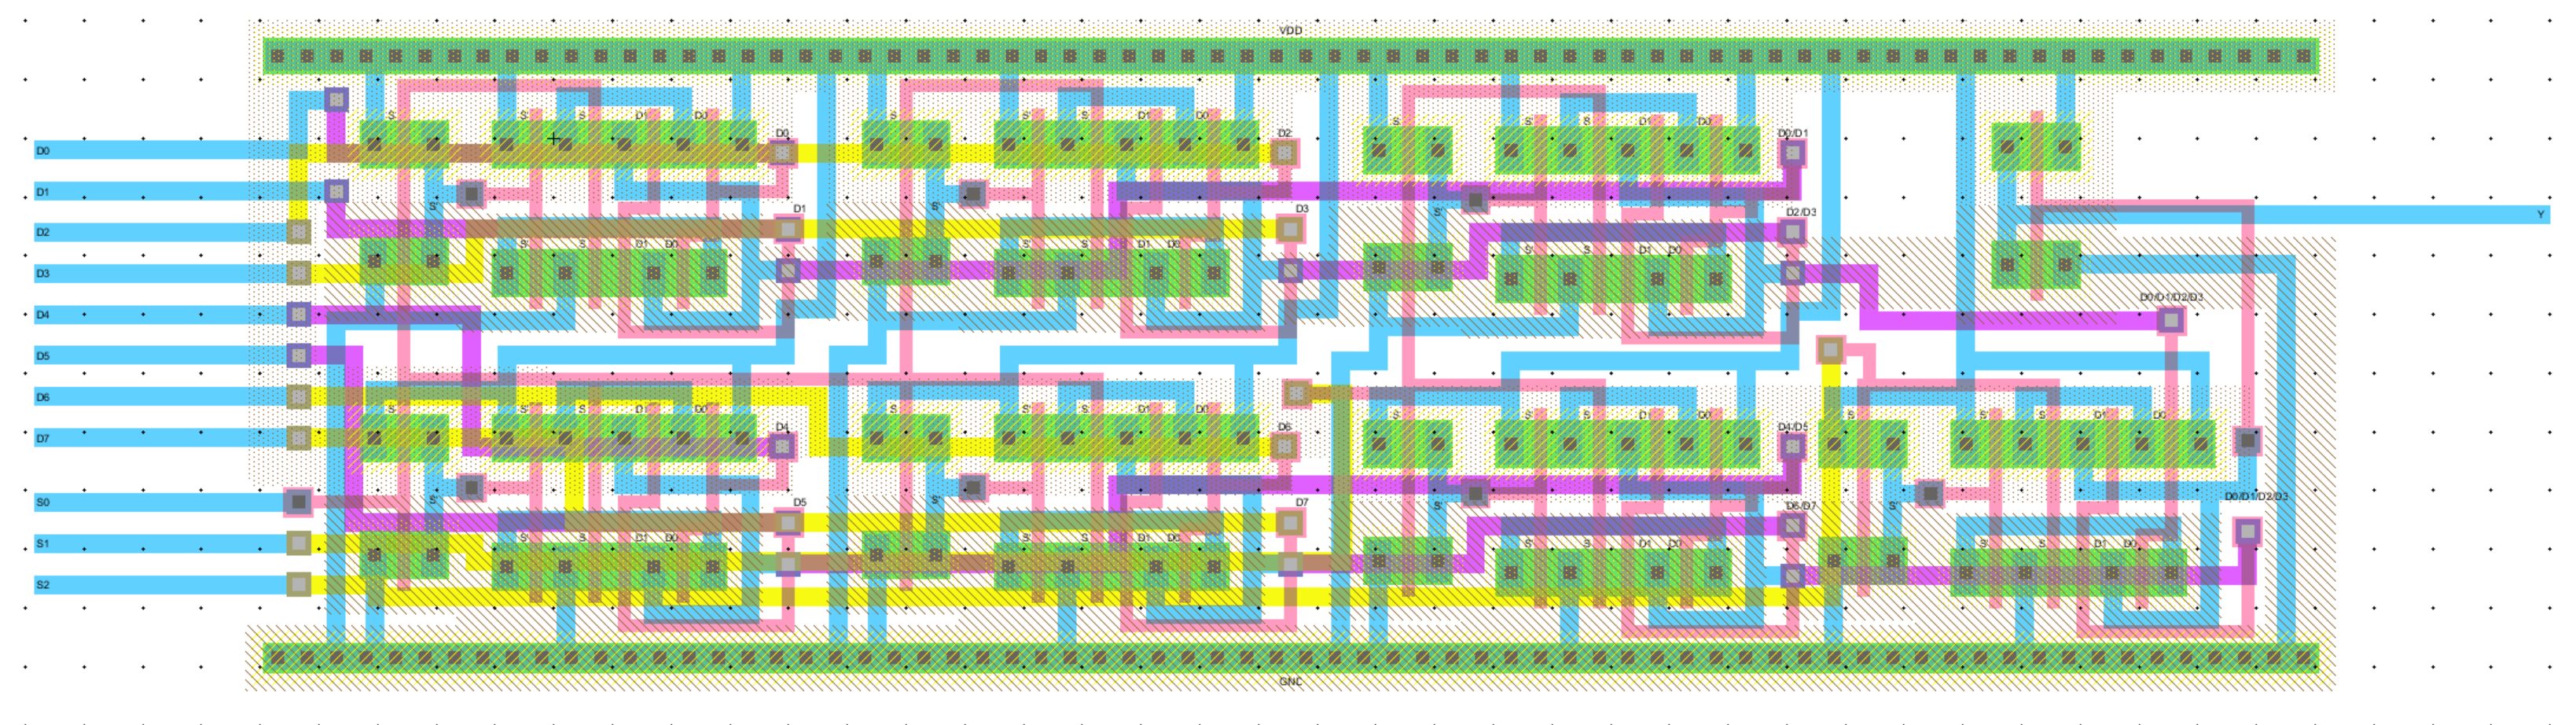
\includegraphics[width=\linewidth, frame]{screenshots/cmos/lay/lay1.png}
      \caption{The layout for the CMOS design of the 8-to-1 multiplexer.}
      \label{fig:cmoslay1}
    \end{figure}


    \begin{figure}[H]
      \centering
      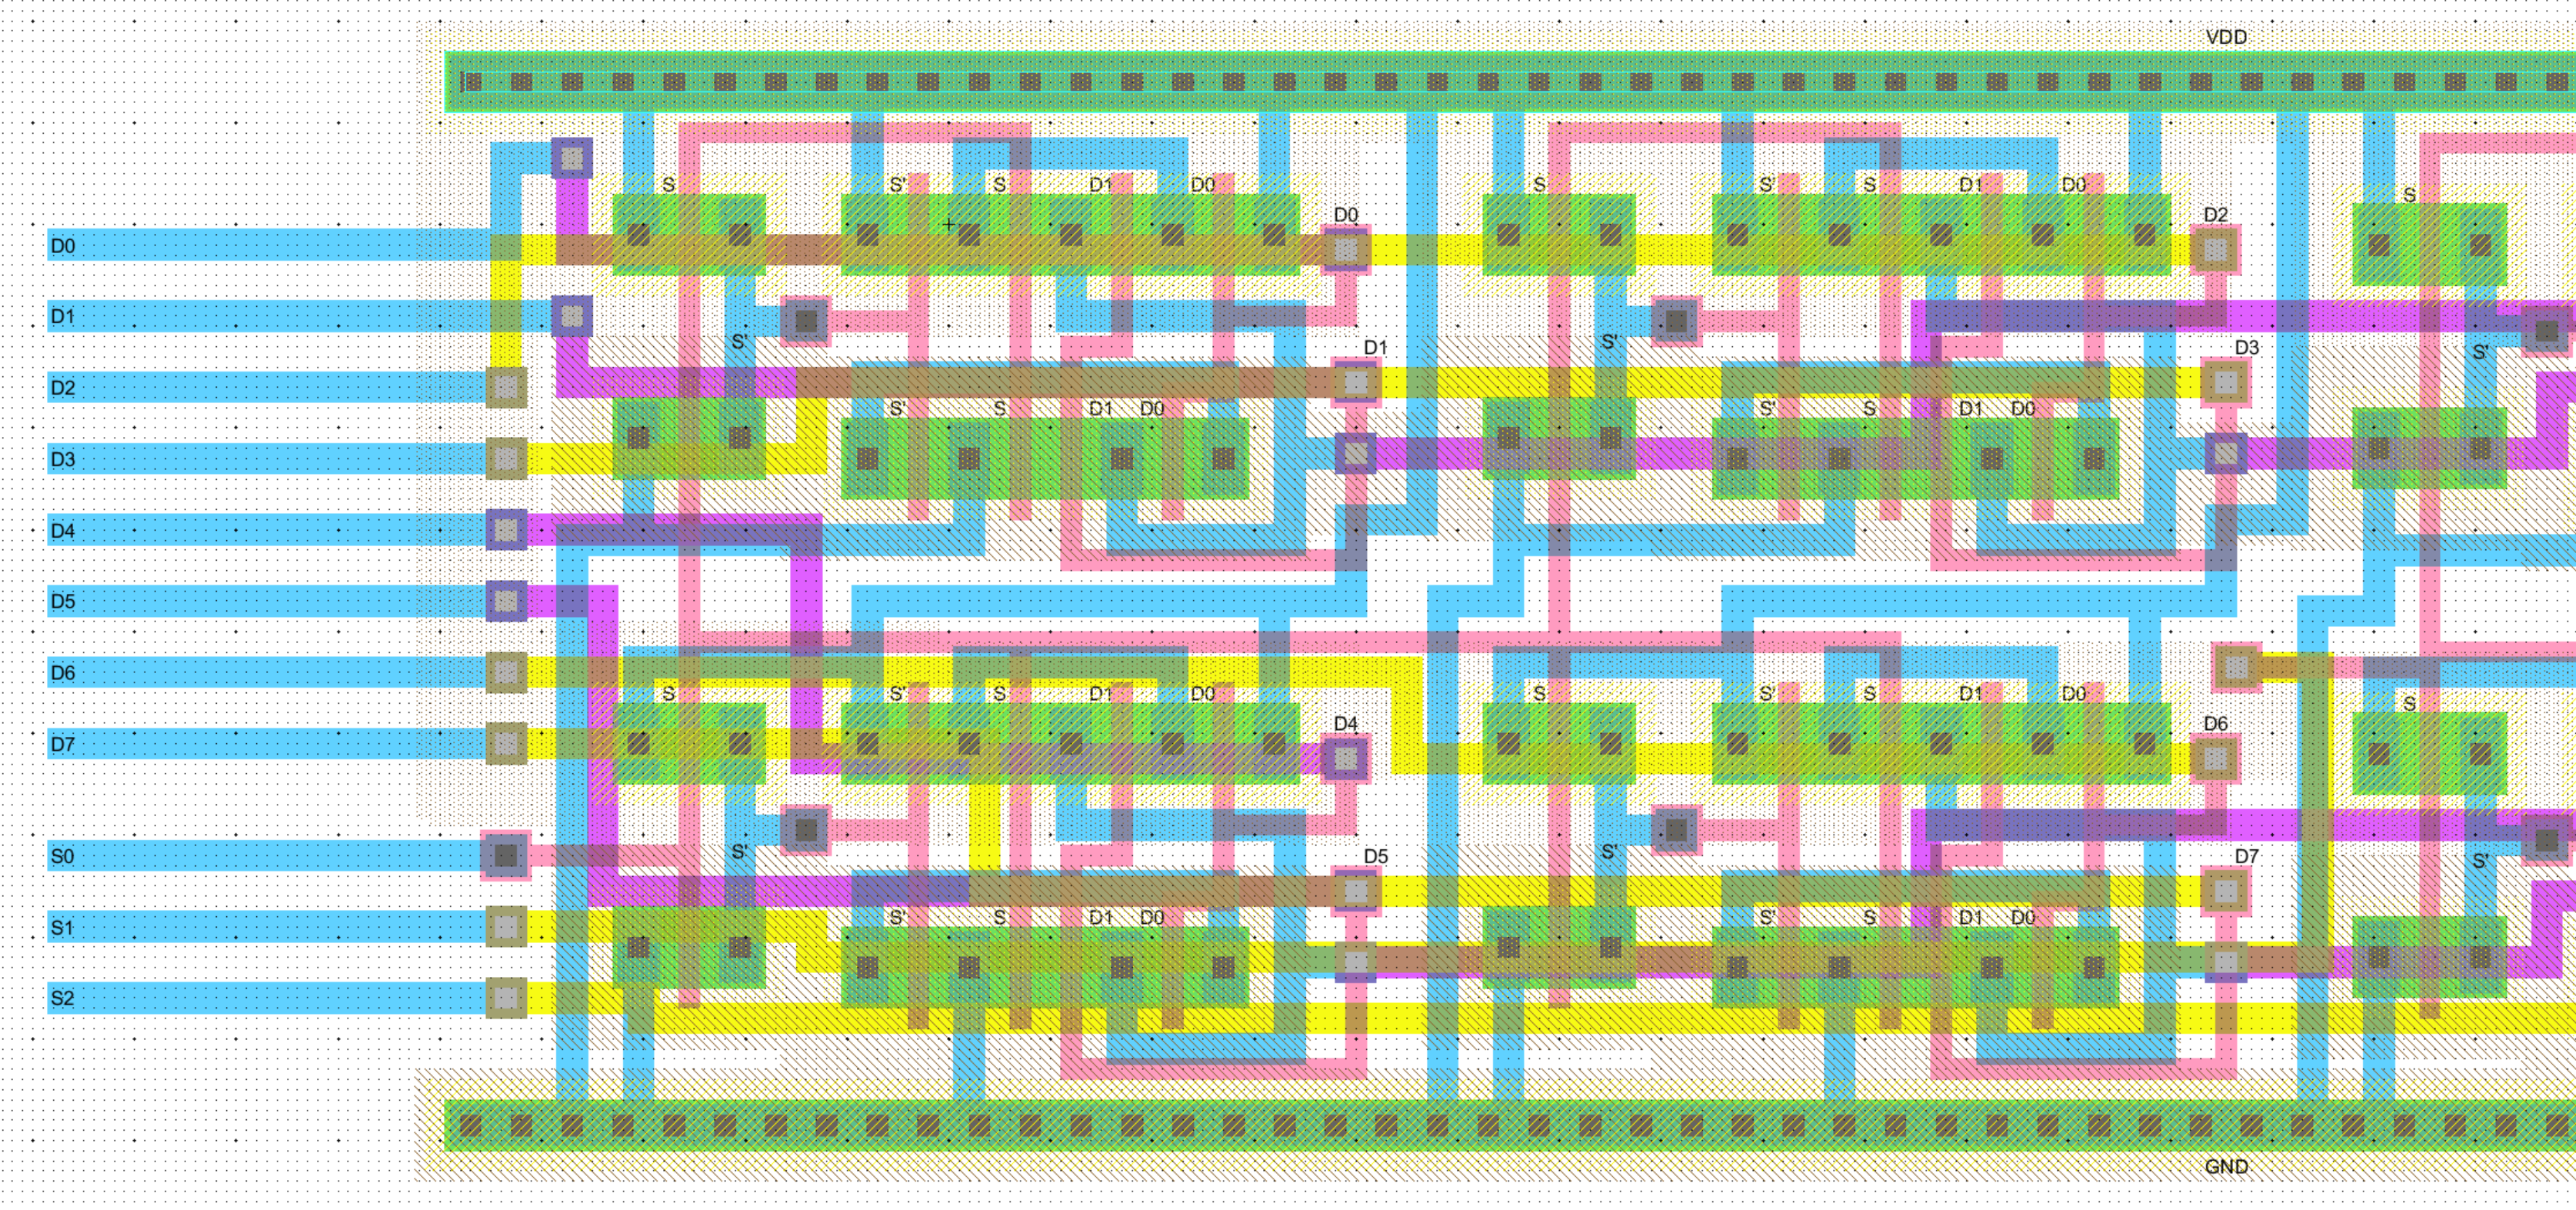
\includegraphics[width=\linewidth, frame]{screenshots/cmos/lay/lay2.png}
      \caption{A close up of the first stage of the multiplexer.}
      \label{fig:cmoslay2}
    \end{figure}

    \begin{figure}[H]
      \centering
      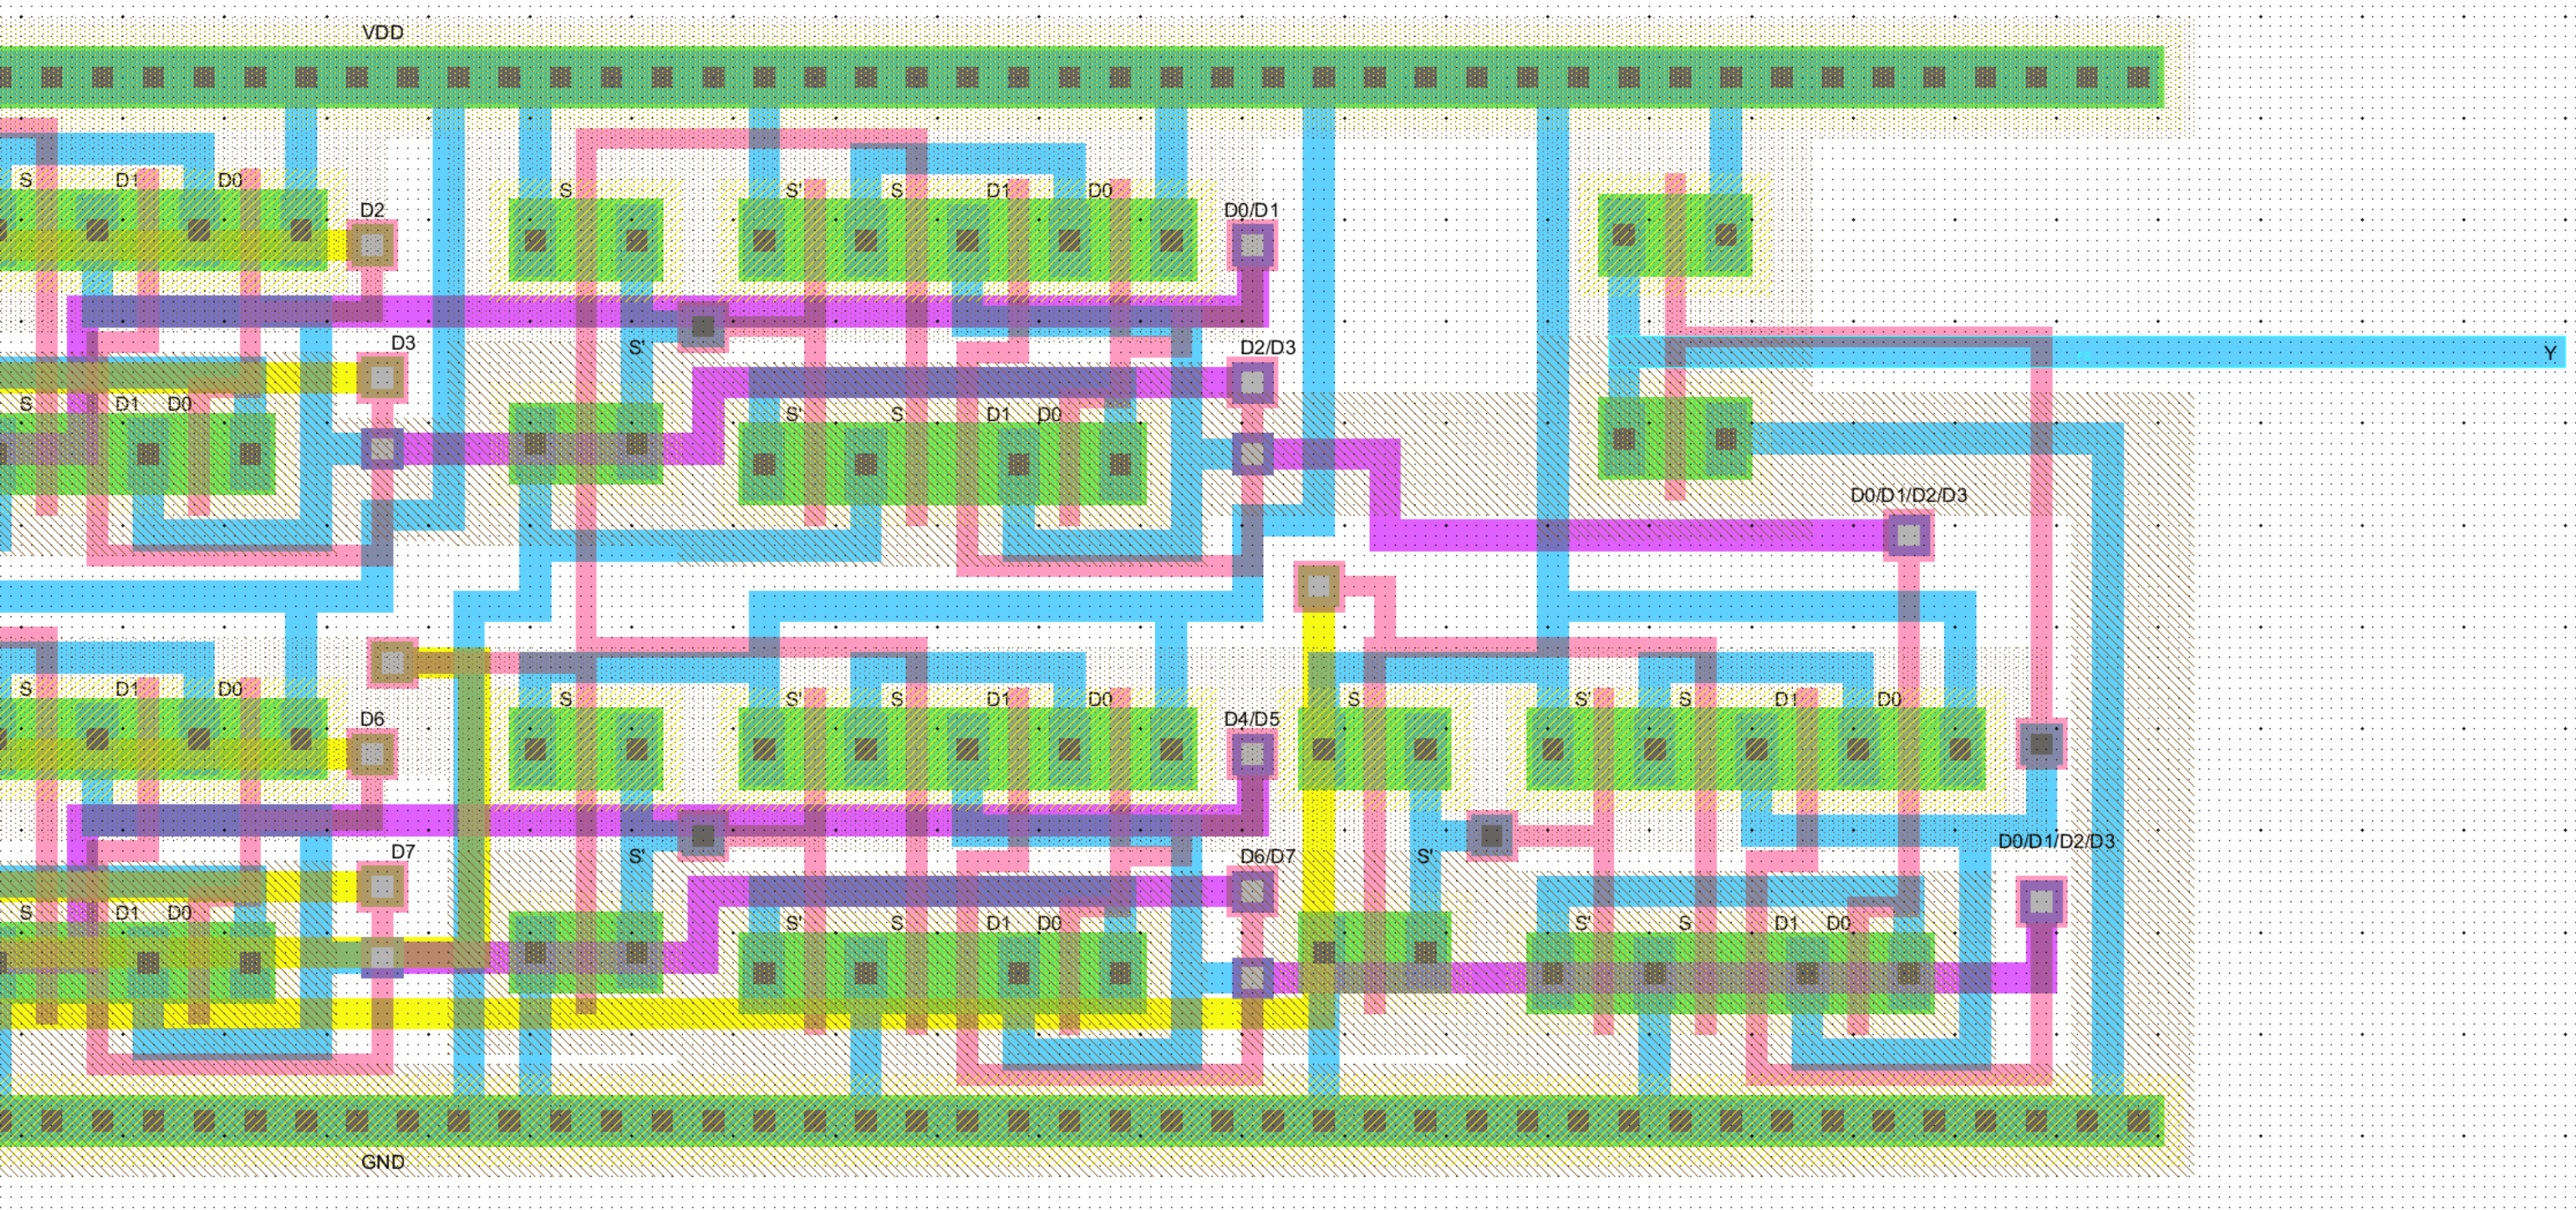
\includegraphics[width=\linewidth, frame]{screenshots/cmos/lay/lay3.png}
      \caption{A close up of the last two stages and final inverter of the multiplexer.}
      \label{fig:cmoslay3}
    \end{figure}

    \paragraph{}
    The DRC results are shown in Figure \ref{fig:cmoslaydrc} and the well check results are shown in Figure \ref{fig:cmoslaywell}, both showing no errors.

    \begin{figure}[H]
      \centering
      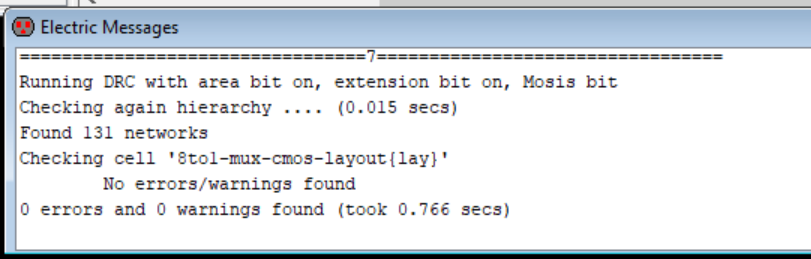
\includegraphics[width=0.6\linewidth, frame]{screenshots/cmos/lay/drc.png}
      \caption{The DRC results for the CMOS layout showing no errors.}
      \label{fig:cmoslaydrc}
    \end{figure}


    \begin{figure}[H]
      \centering
      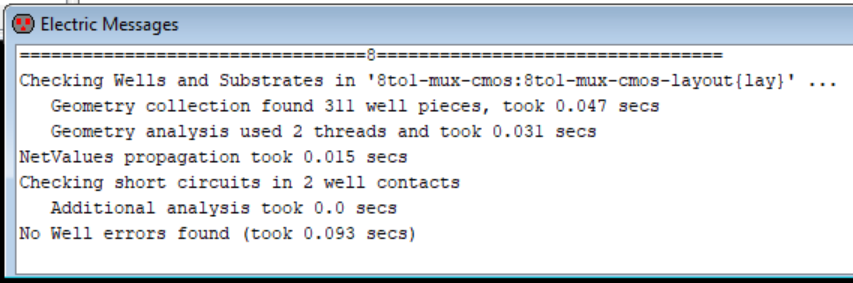
\includegraphics[width=0.6\linewidth, frame]{screenshots/cmos/lay/well.png}
      \caption{The well check results for the CMOS layout showing no errors.}
      \label{fig:cmoslaywell}
    \end{figure}


\section{LTSpice Simulation for Layout}
  \paragraph{}
  This section will detail the LTSpice simulations for both the transmission gate schematic and the CMOS layouts. As previously mentioned, the spice code used to generate the graphs for this simulation are shown in Figure \ref{fig:simcode} and the code used to generate the measurements is shown in Figure \ref{fig:meascode}.


  \subsection{Transmission Gate Layout LTSpice}
    \paragraph{}
    The spice simulation for the transmission gate layout is shown in Figure \ref{fig:tglayspice}. As described in previous sections, the behavior in the graph is as expected. Each input is passed through to the output when selected by the select line.

    \begin{figure}[H]
      \centering
      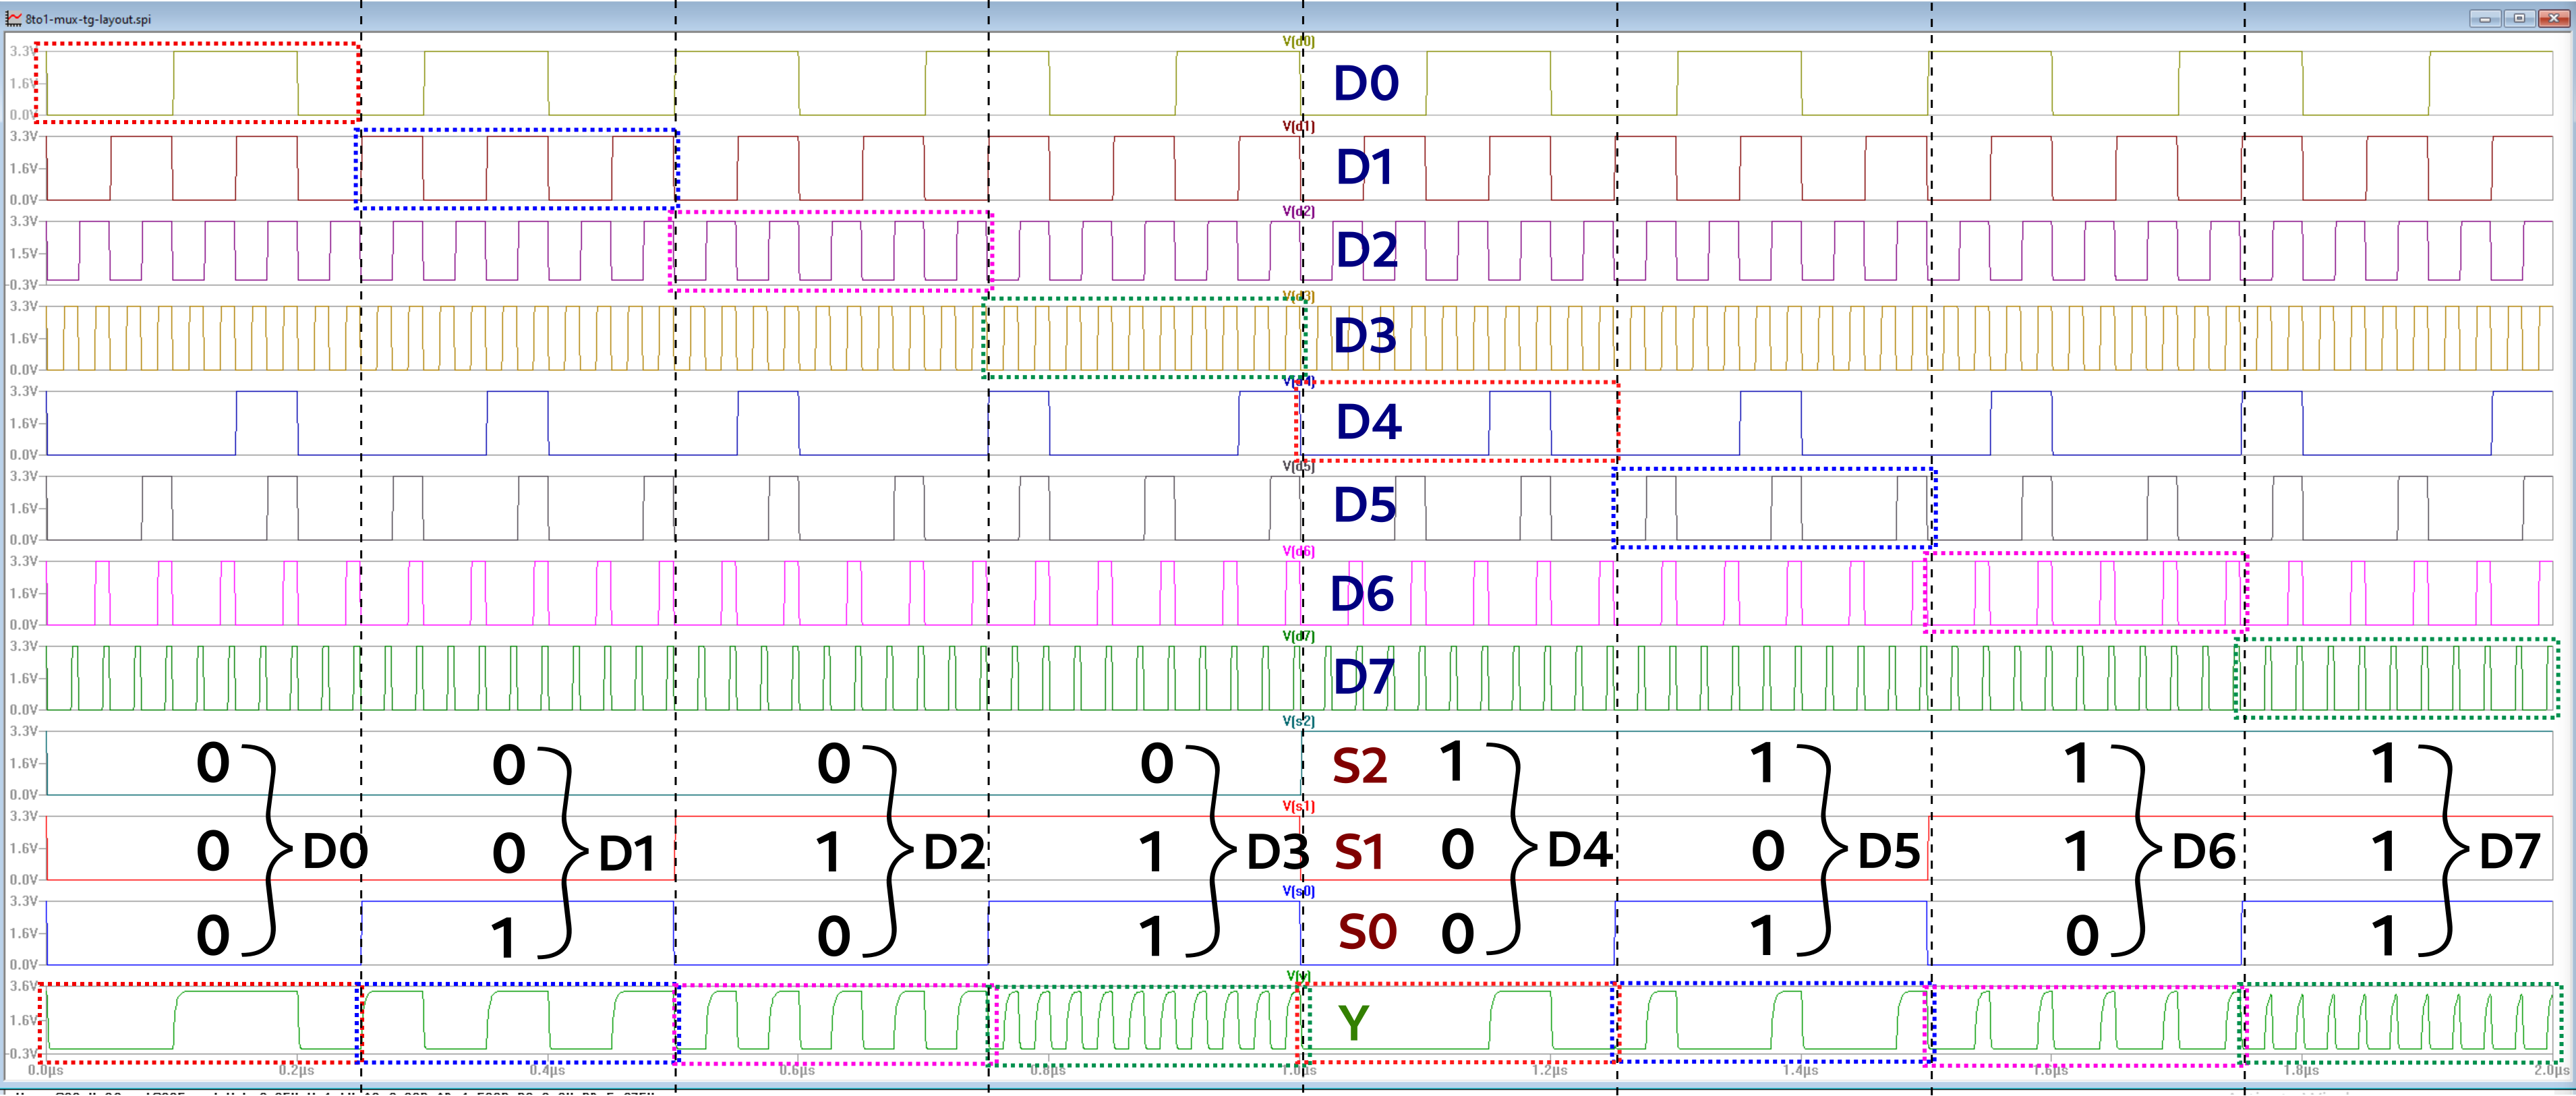
\includegraphics[width=\linewidth, frame]{screenshots/tg/lay/spice.png}
      \caption{The LTSpice simulation of the transmission gate layout showing that each combination of inputs to the select line passes through the corresponding inputs D0 through D7.}
      \label{fig:tglayspice}
    \end{figure}

    \paragraph{}
    The measurements obtained with the spice code shown in Figure \ref{fig:meascode} for the transmission gate layout are shown in Figure \ref{fig:tglaymeas}.

    \begin{figure}[H]
      \centering
      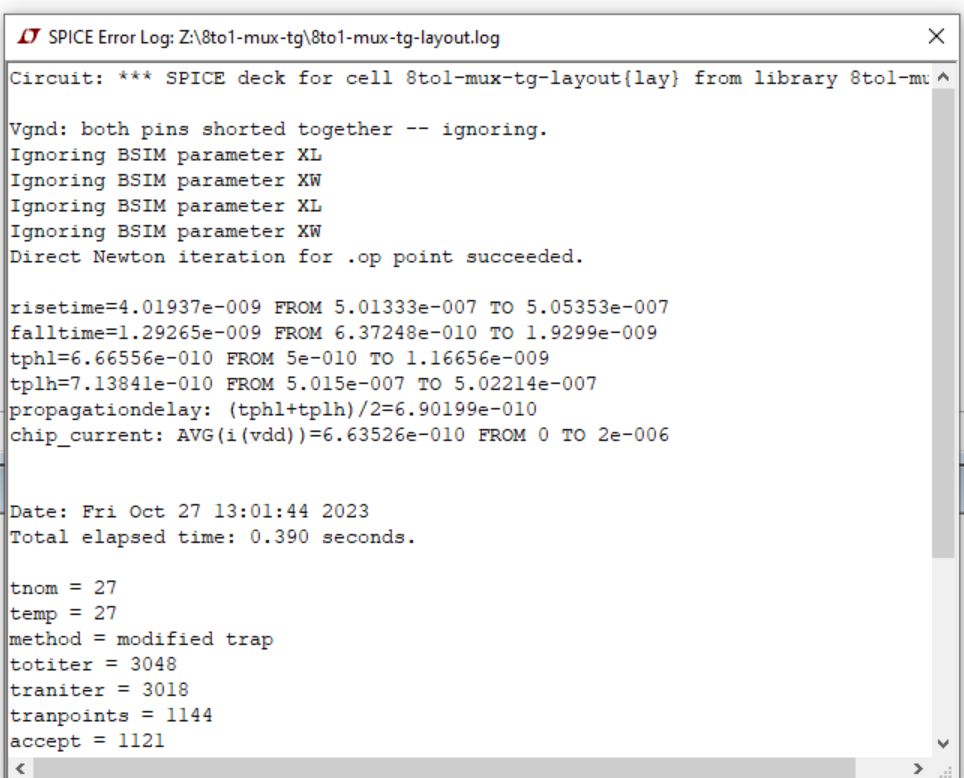
\includegraphics[width=0.5\linewidth, frame]{screenshots/tg/lay/meas.png}
      \caption{The measurements obtained through LTSpice simulation of the transmission gate layout.}
      \label{fig:tglaymeas}
    \end{figure}


  \subsection{CMOS Layout LTSpice}
    \paragraph{}
    The spice simulation for the CMOS layout is shown in Figure \ref{fig:cmoslayspice}. As described in previous sections, the behavior in the graph is as expected. Each input is passed through to the output when selected by the select line.

    \begin{figure}[H]
      \centering
      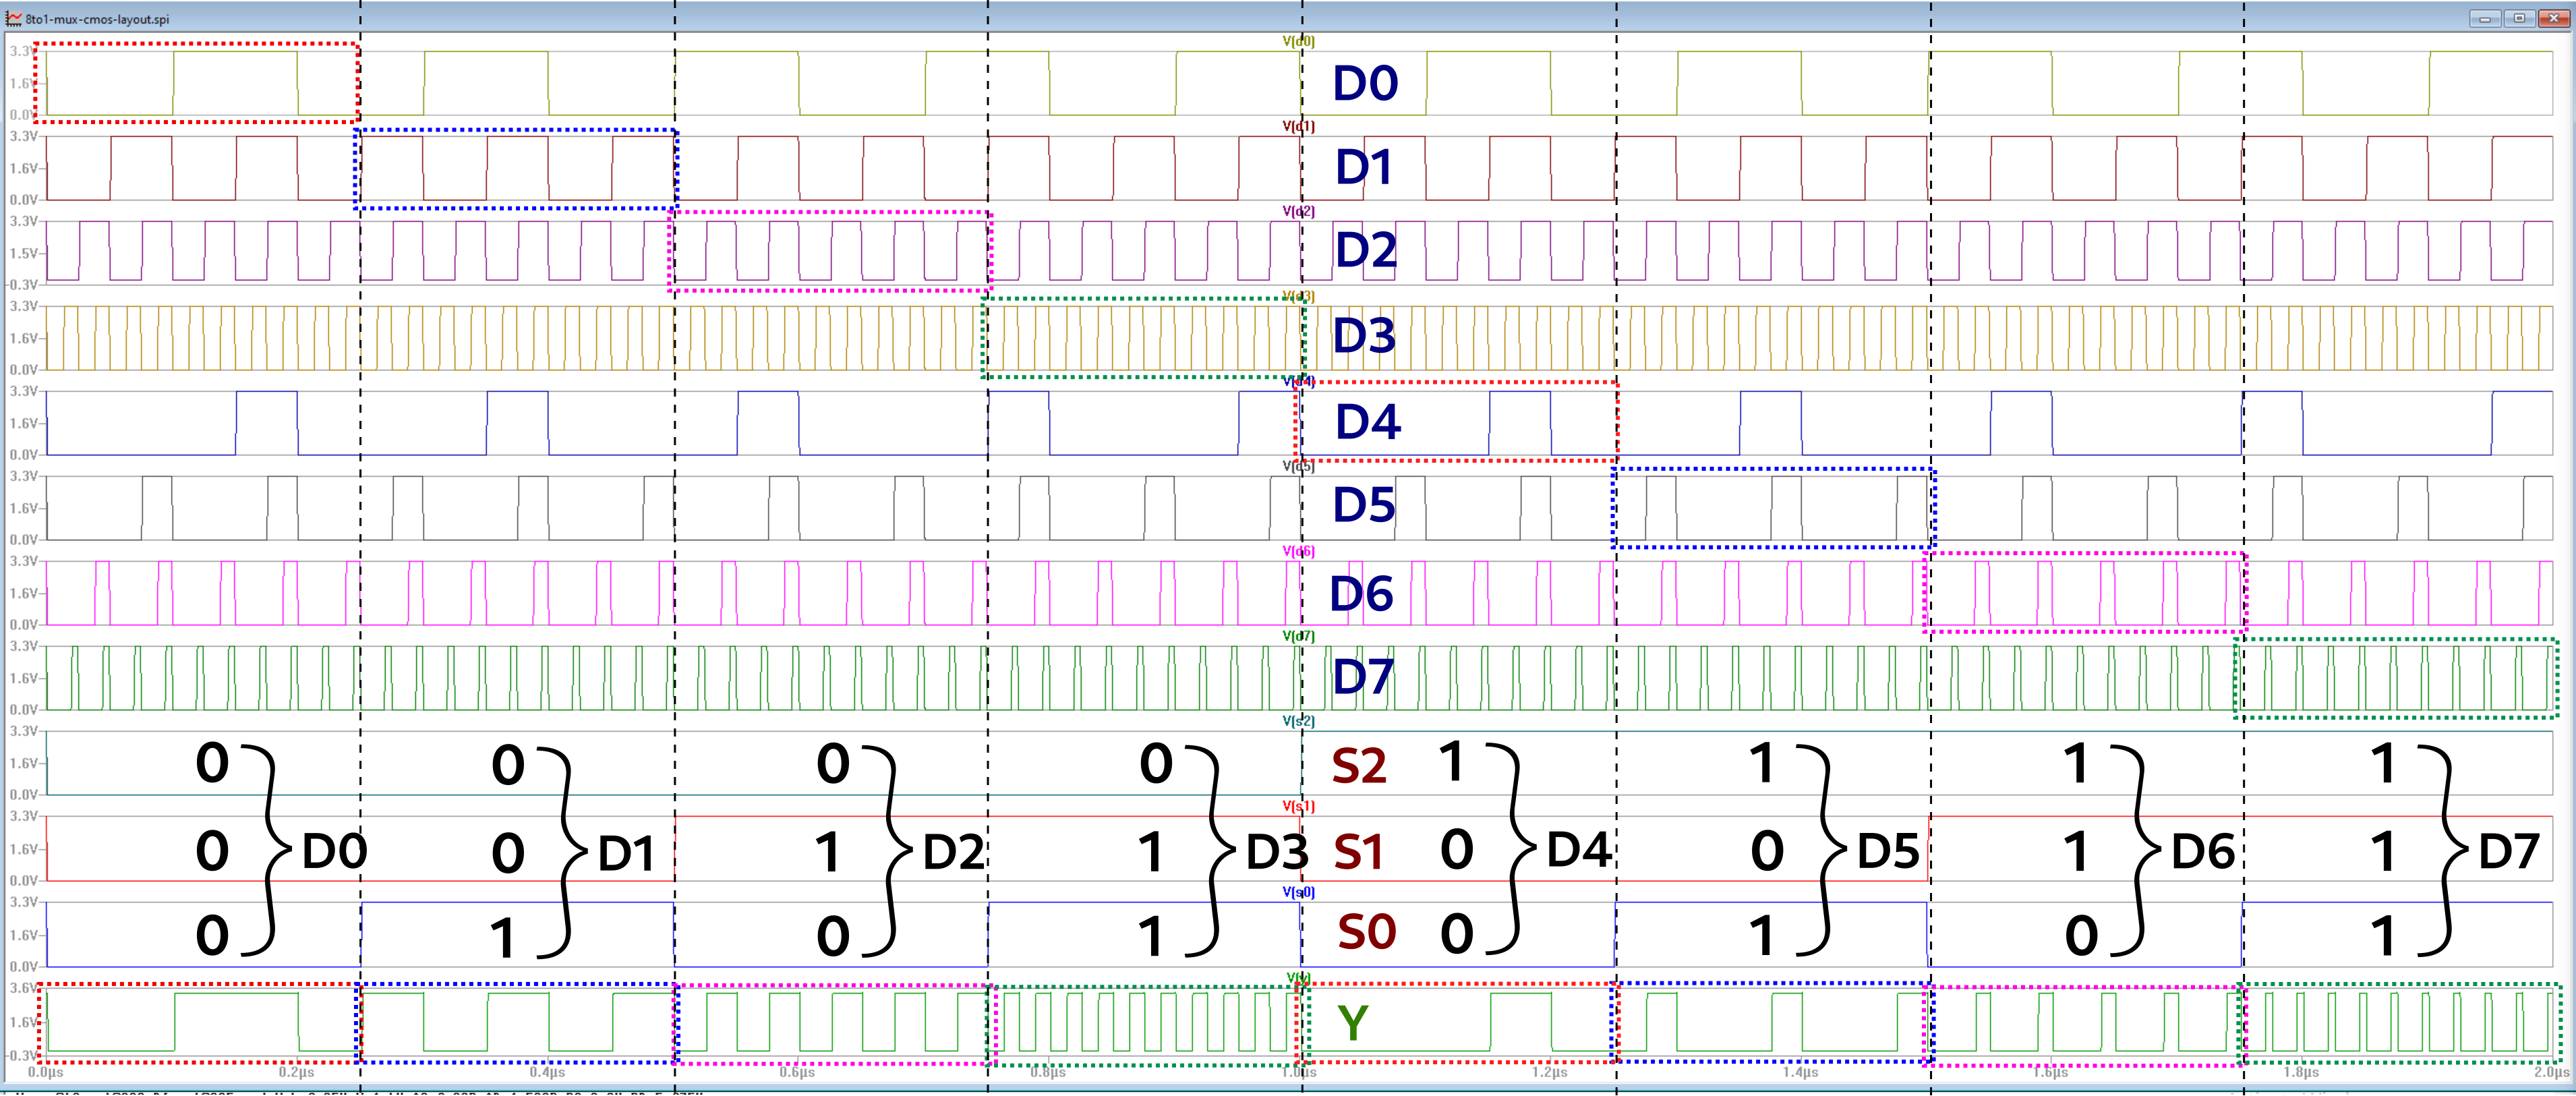
\includegraphics[width=\linewidth, frame]{screenshots/cmos/lay/spice.png}
      \caption{The LTSpice simulation of the CMOS layout showing that each combination of inputs to the select line passes through the corresponding inputs D0 through D7.}
      \label{fig:cmoslayspice}
    \end{figure}

    \paragraph{}
    The measurements obtained with the spice code shown in Figure \ref{fig:meascode} for the CMOS layout are shown in Figure \ref{fig:cmoslaymeas}.

    \begin{figure}[H]
      \centering
      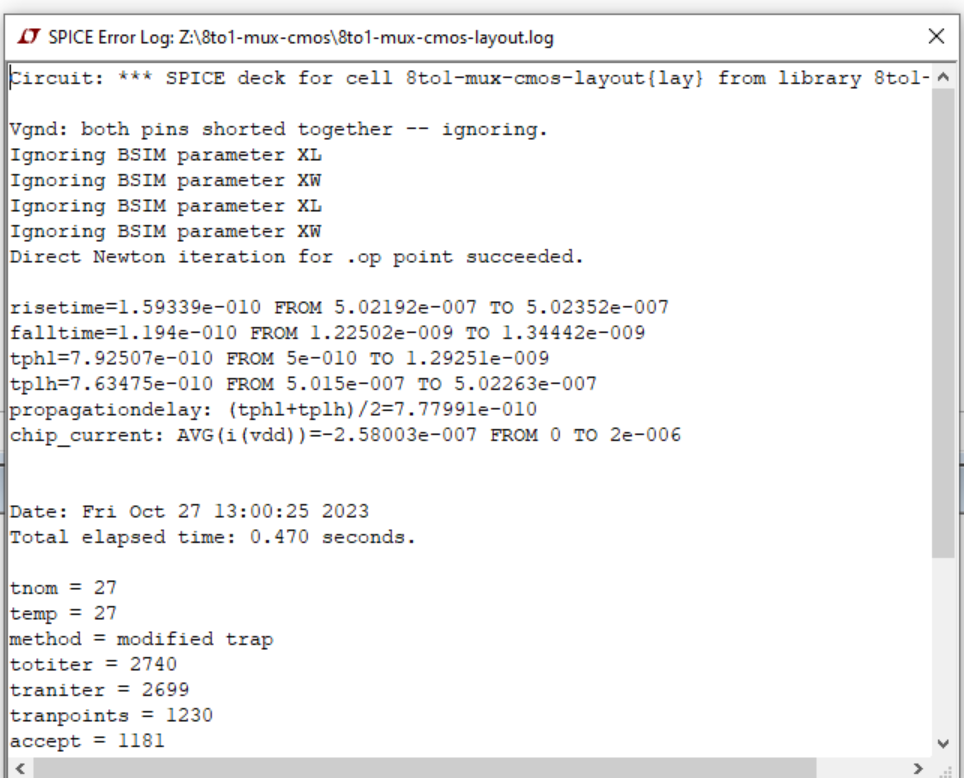
\includegraphics[width=0.5\linewidth, frame]{screenshots/cmos/lay/meas.png}
      \caption{The measurements obtained through LTSpice simulation of the CMOS layout.}
      \label{fig:cmoslaymeas}
    \end{figure}



\section{IRSIM for Layout}
  \paragraph{}
  This section details the IRSIM simulations done on both the transmission gate layout and the CMOS layout. As mentioned previously, I chose to simulate only one D input per screenshot and two per design. This is because IRSIM can be buggy and has a hard time with too many inputs changing at once.  

  \subsection{Transmission Gate Layout IRSIM}
    \paragraph{}
    The IRSIM simulation for the transmission gate layout is shown in Figure \ref{fig:tglayirsim1} and \ref{fig:tglayirsim2}. As shown in the screenshots, the layout behaves as expected.

    \begin{figure}[H]
      \centering
      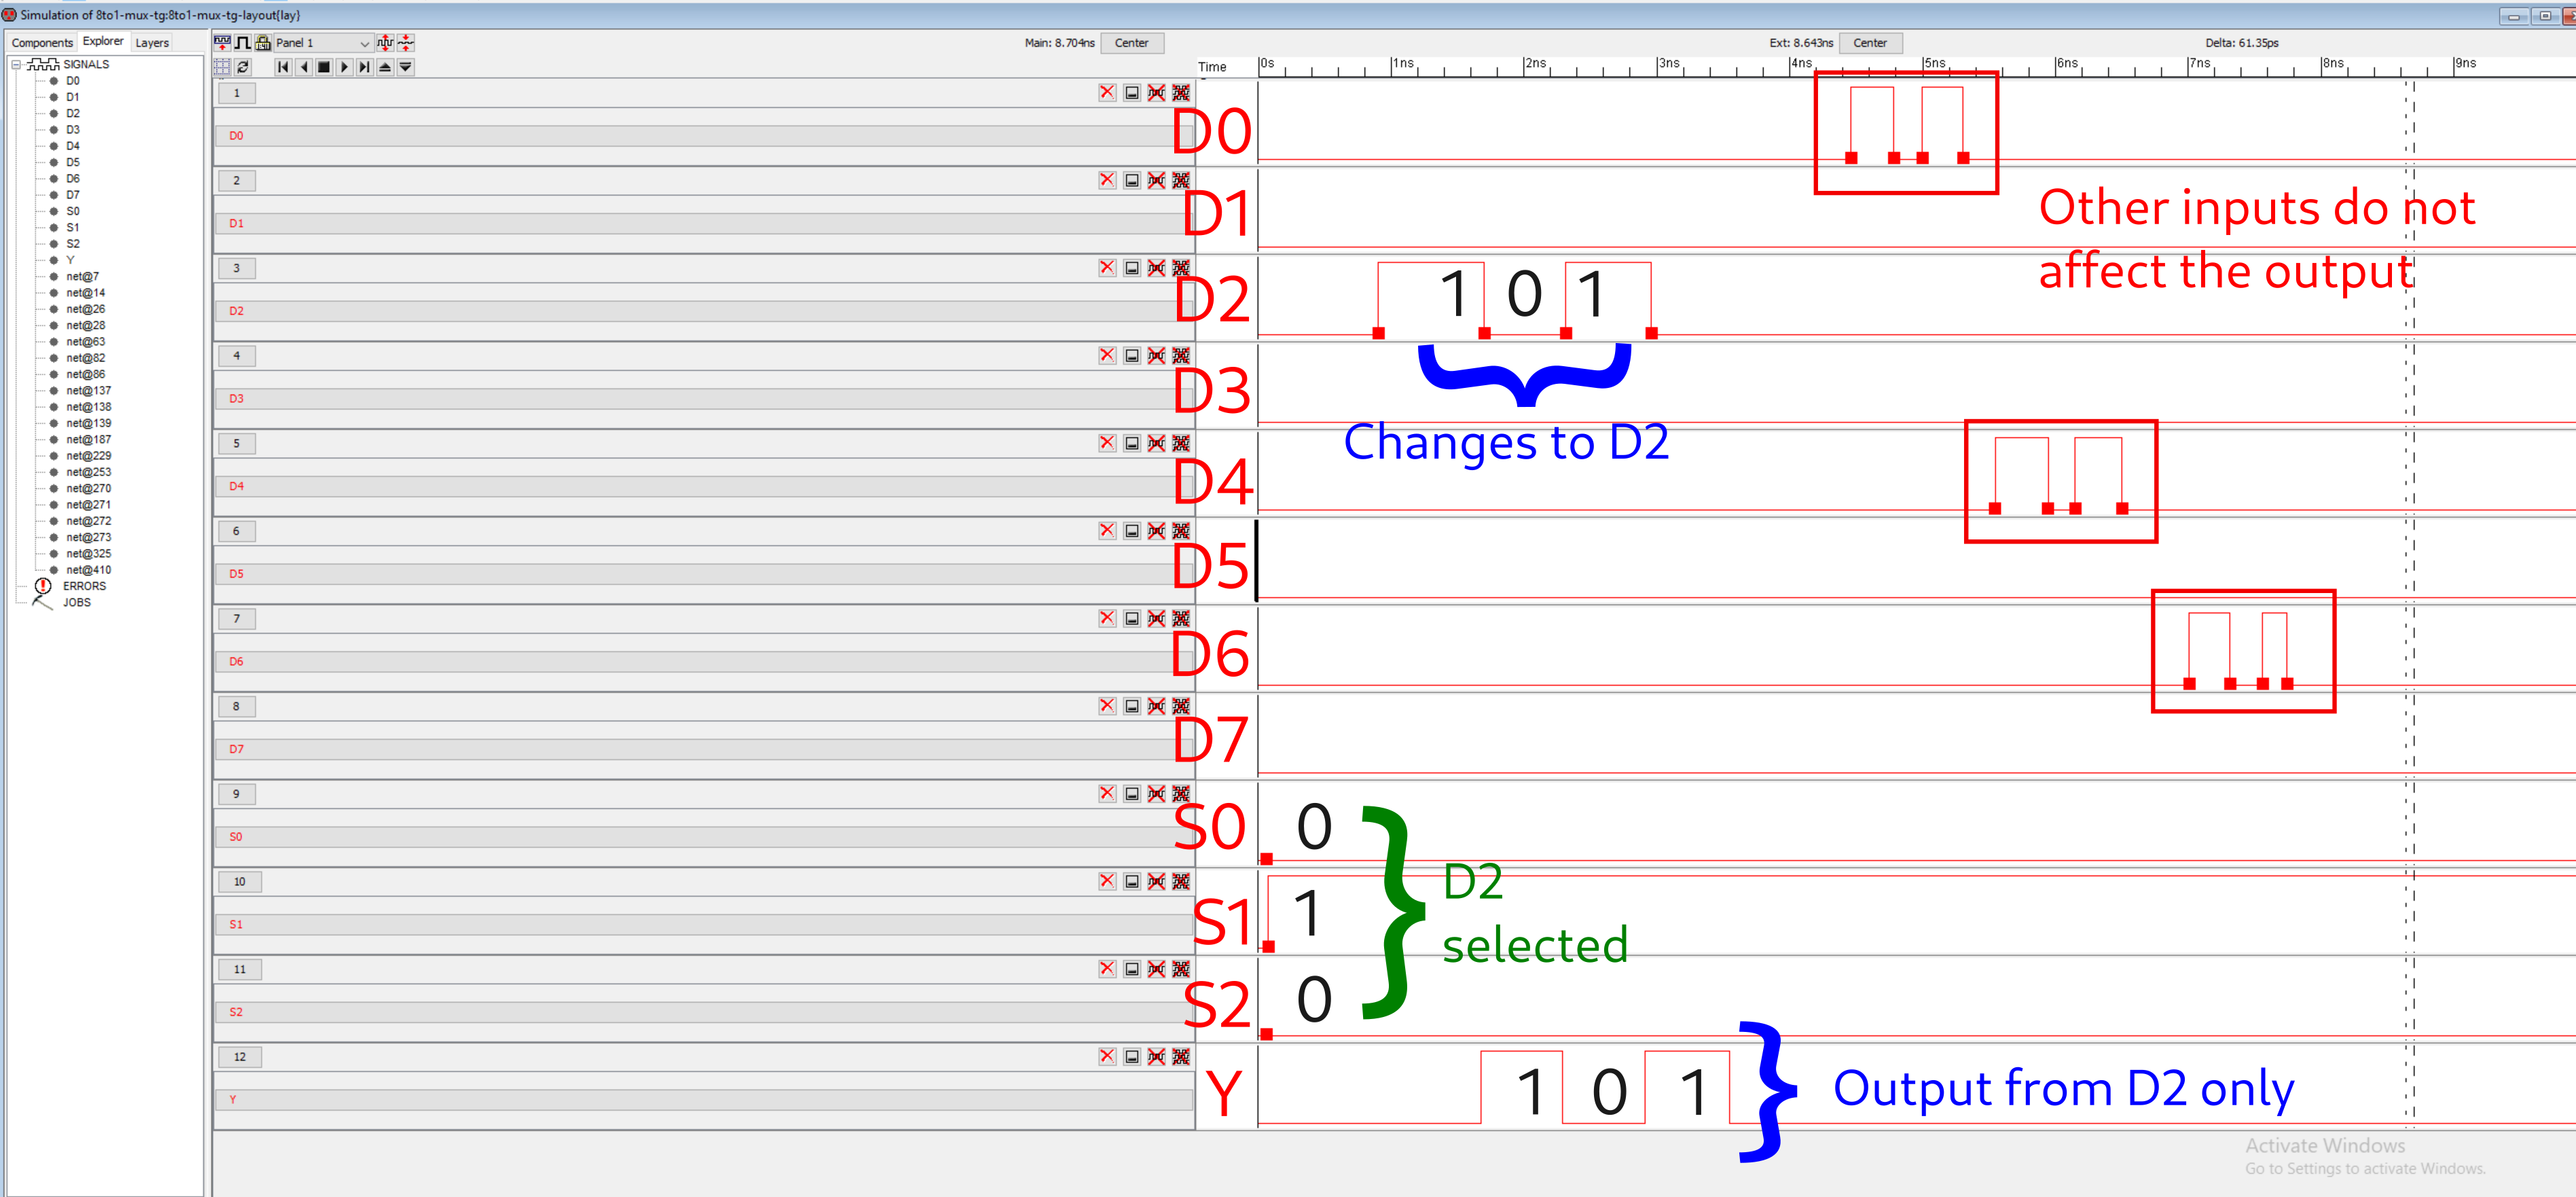
\includegraphics[width=\linewidth, frame]{screenshots/tg/lay/irsim.png}
      \caption{One IRSIM simulation for the transmission gate layout showing that the design works as expected.}
      \label{fig:tglayirsim1}
    \end{figure}


    \begin{figure}[H]
      \centering
      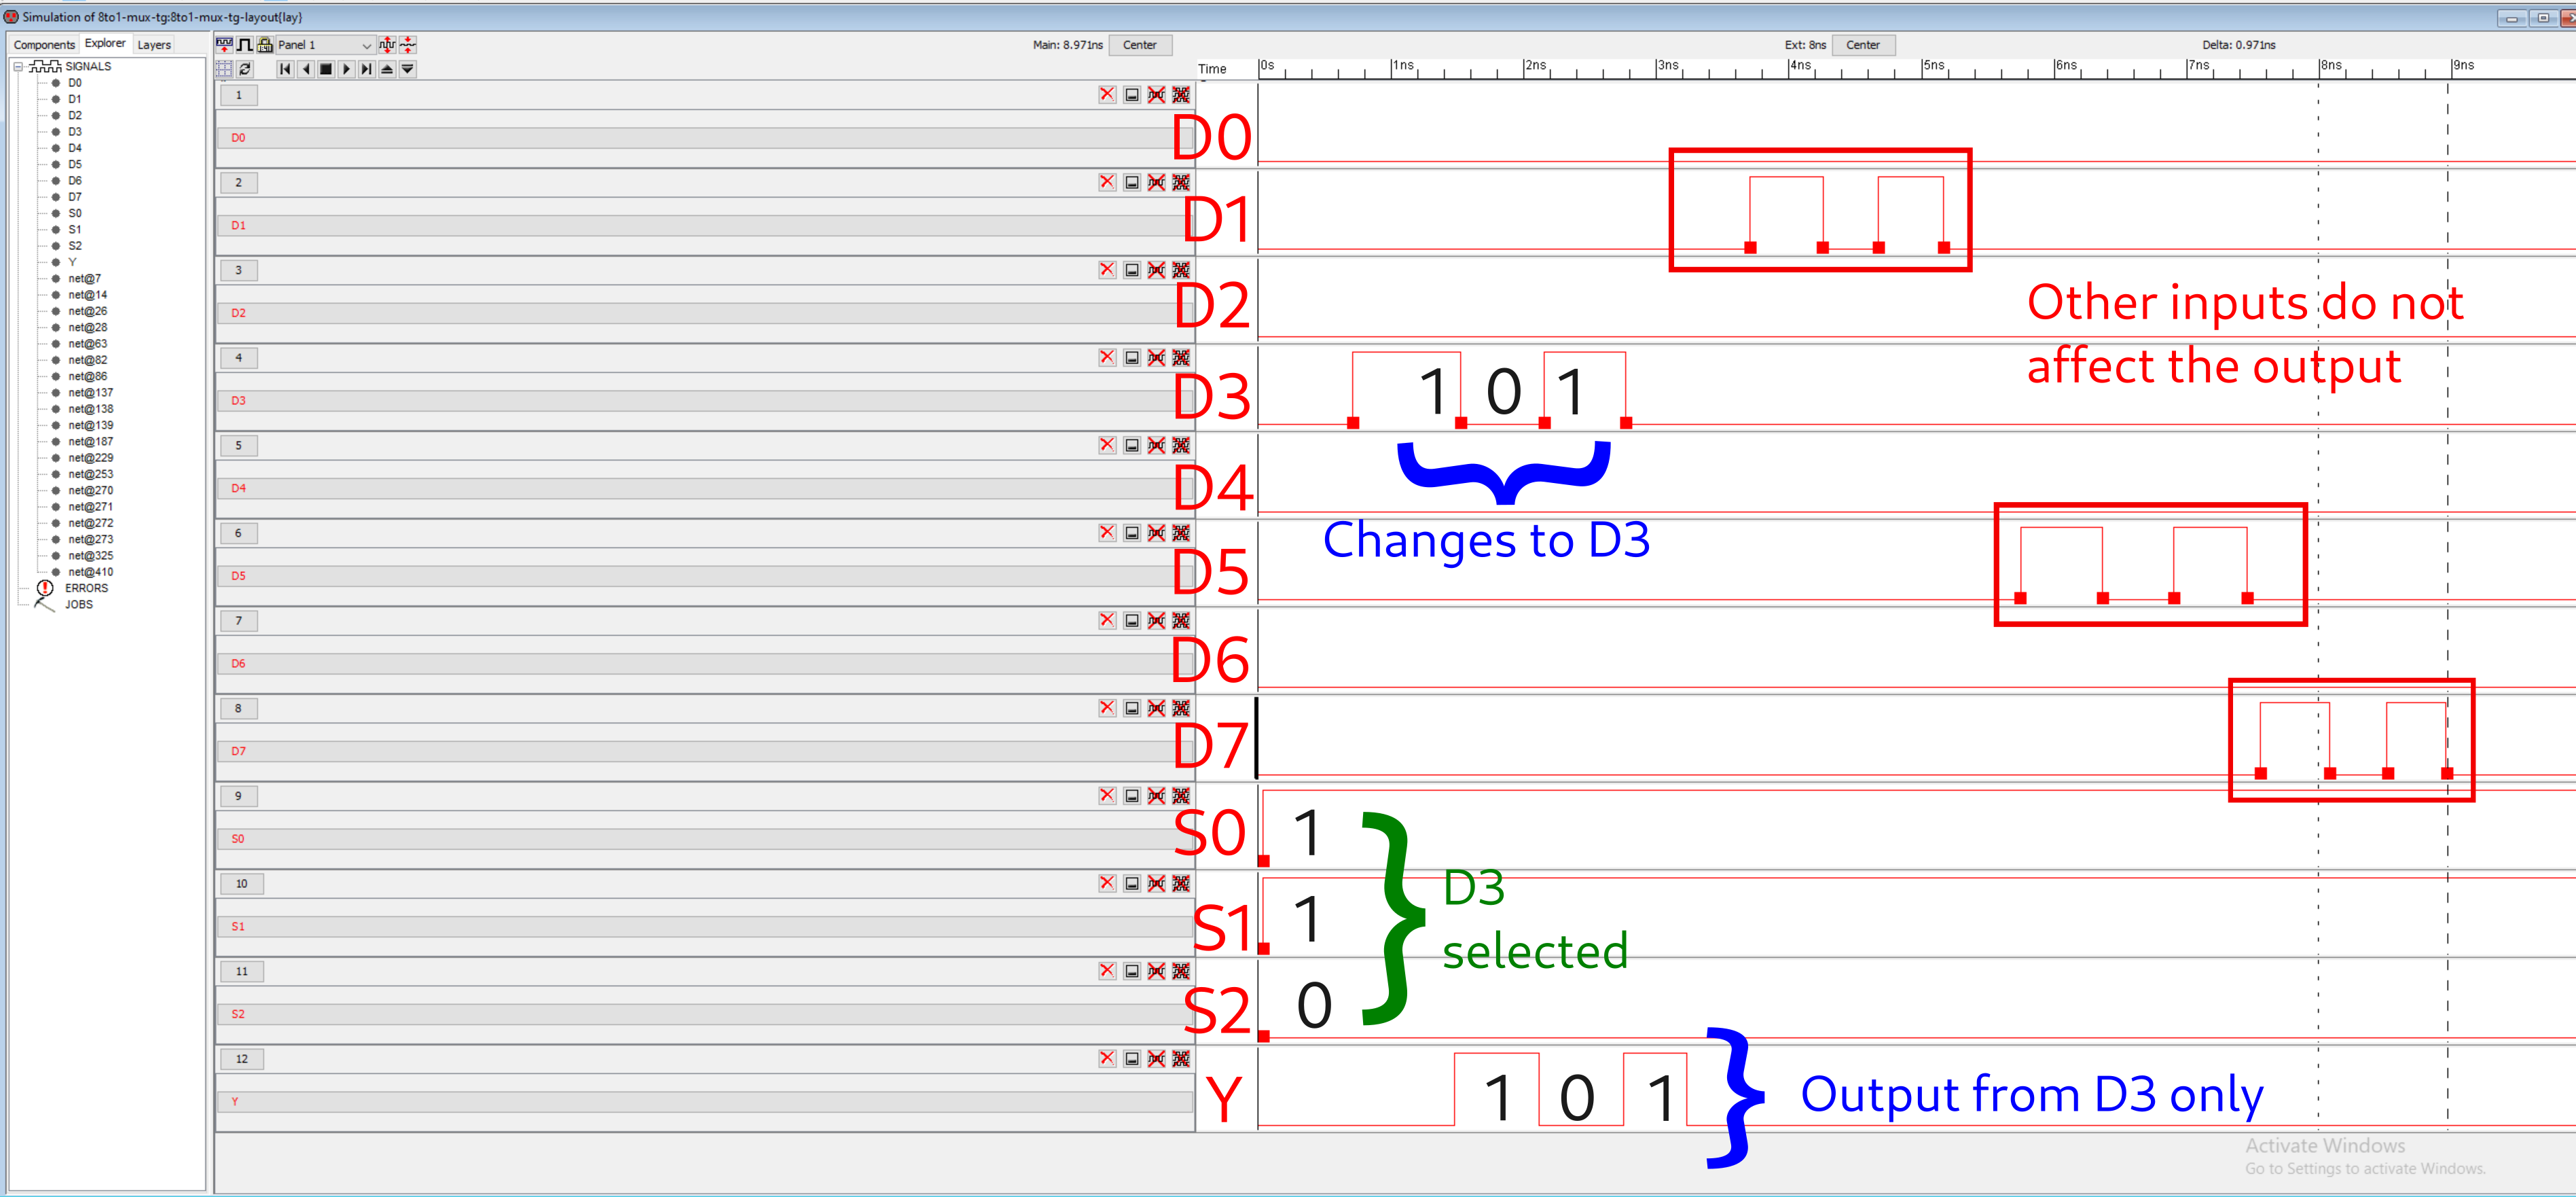
\includegraphics[width=\linewidth, frame]{screenshots/tg/lay/irsim2.png}
      \caption{Another IRSIM simulation for the transmission gate layout showing that the design works as expected.}
      \label{fig:tglayirsim2}
    \end{figure}


  \subsection{CMOS Layout IRSIM}
    \paragraph{}
    The IRSIM simulation for the CMOS layout is shown in Figure \ref{fig:cmoslayirsim1} and \ref{fig:cmoslayirsim2}. As shown in the screenshots, the layout behaves as expected.

    \begin{figure}[H]
      \centering
      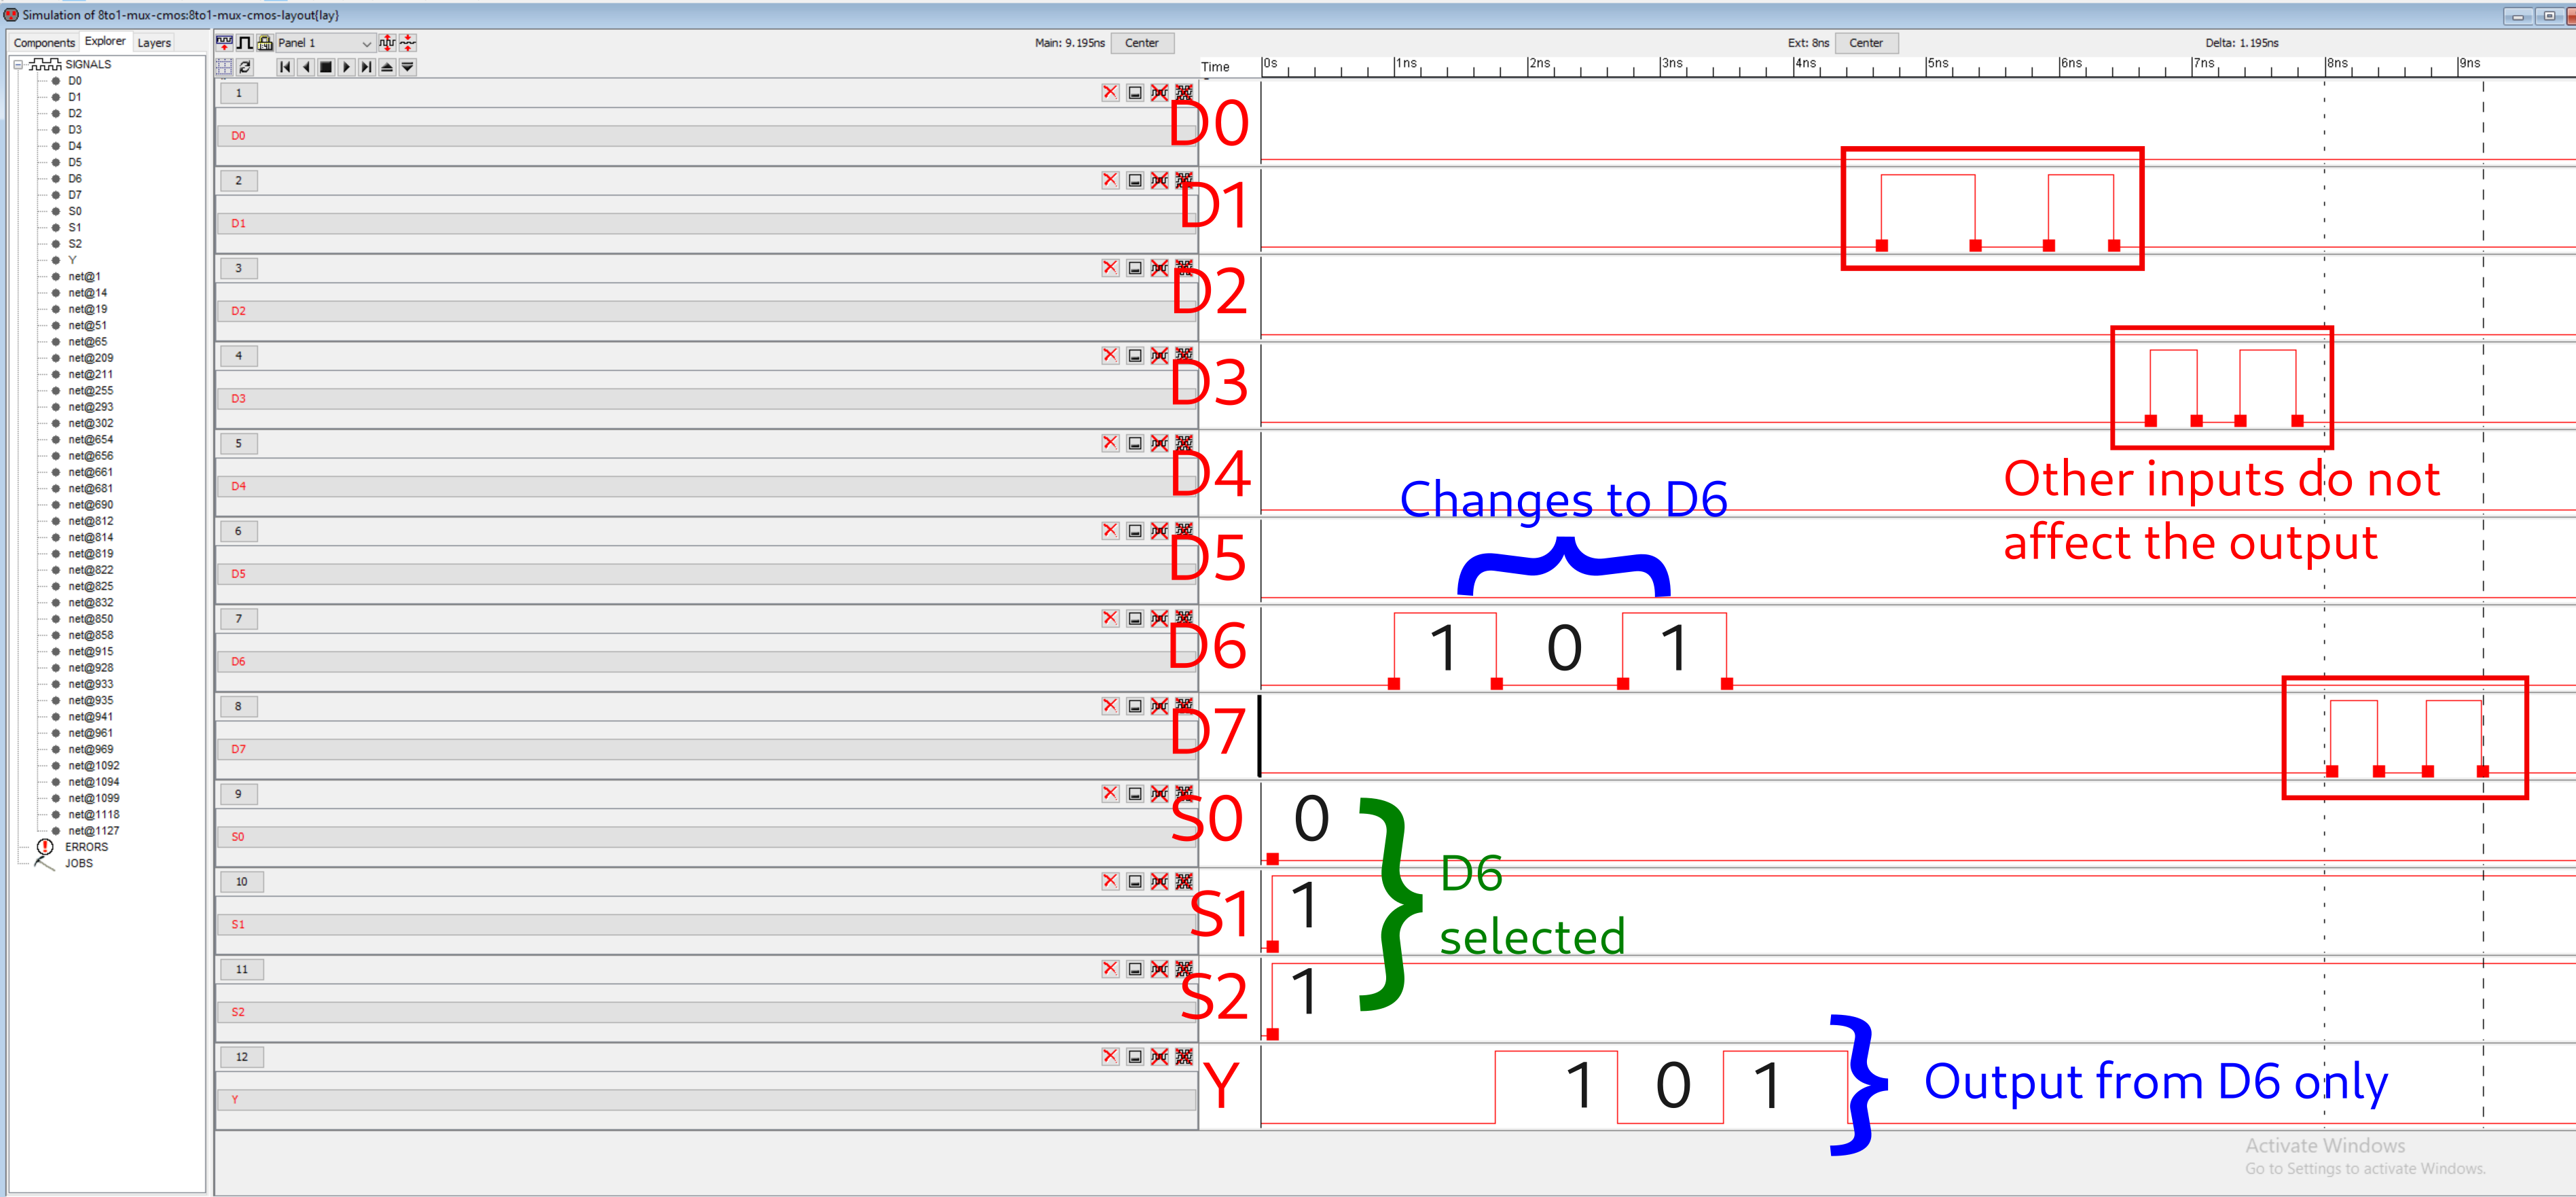
\includegraphics[width=\linewidth, frame]{screenshots/cmos/lay/irsim.png}
      \caption{One IRSIM simulation for the CMOS layout showing that the design works as expected.}
      \label{fig:cmoslayirsim1}
    \end{figure}


    \begin{figure}[H]
      \centering
      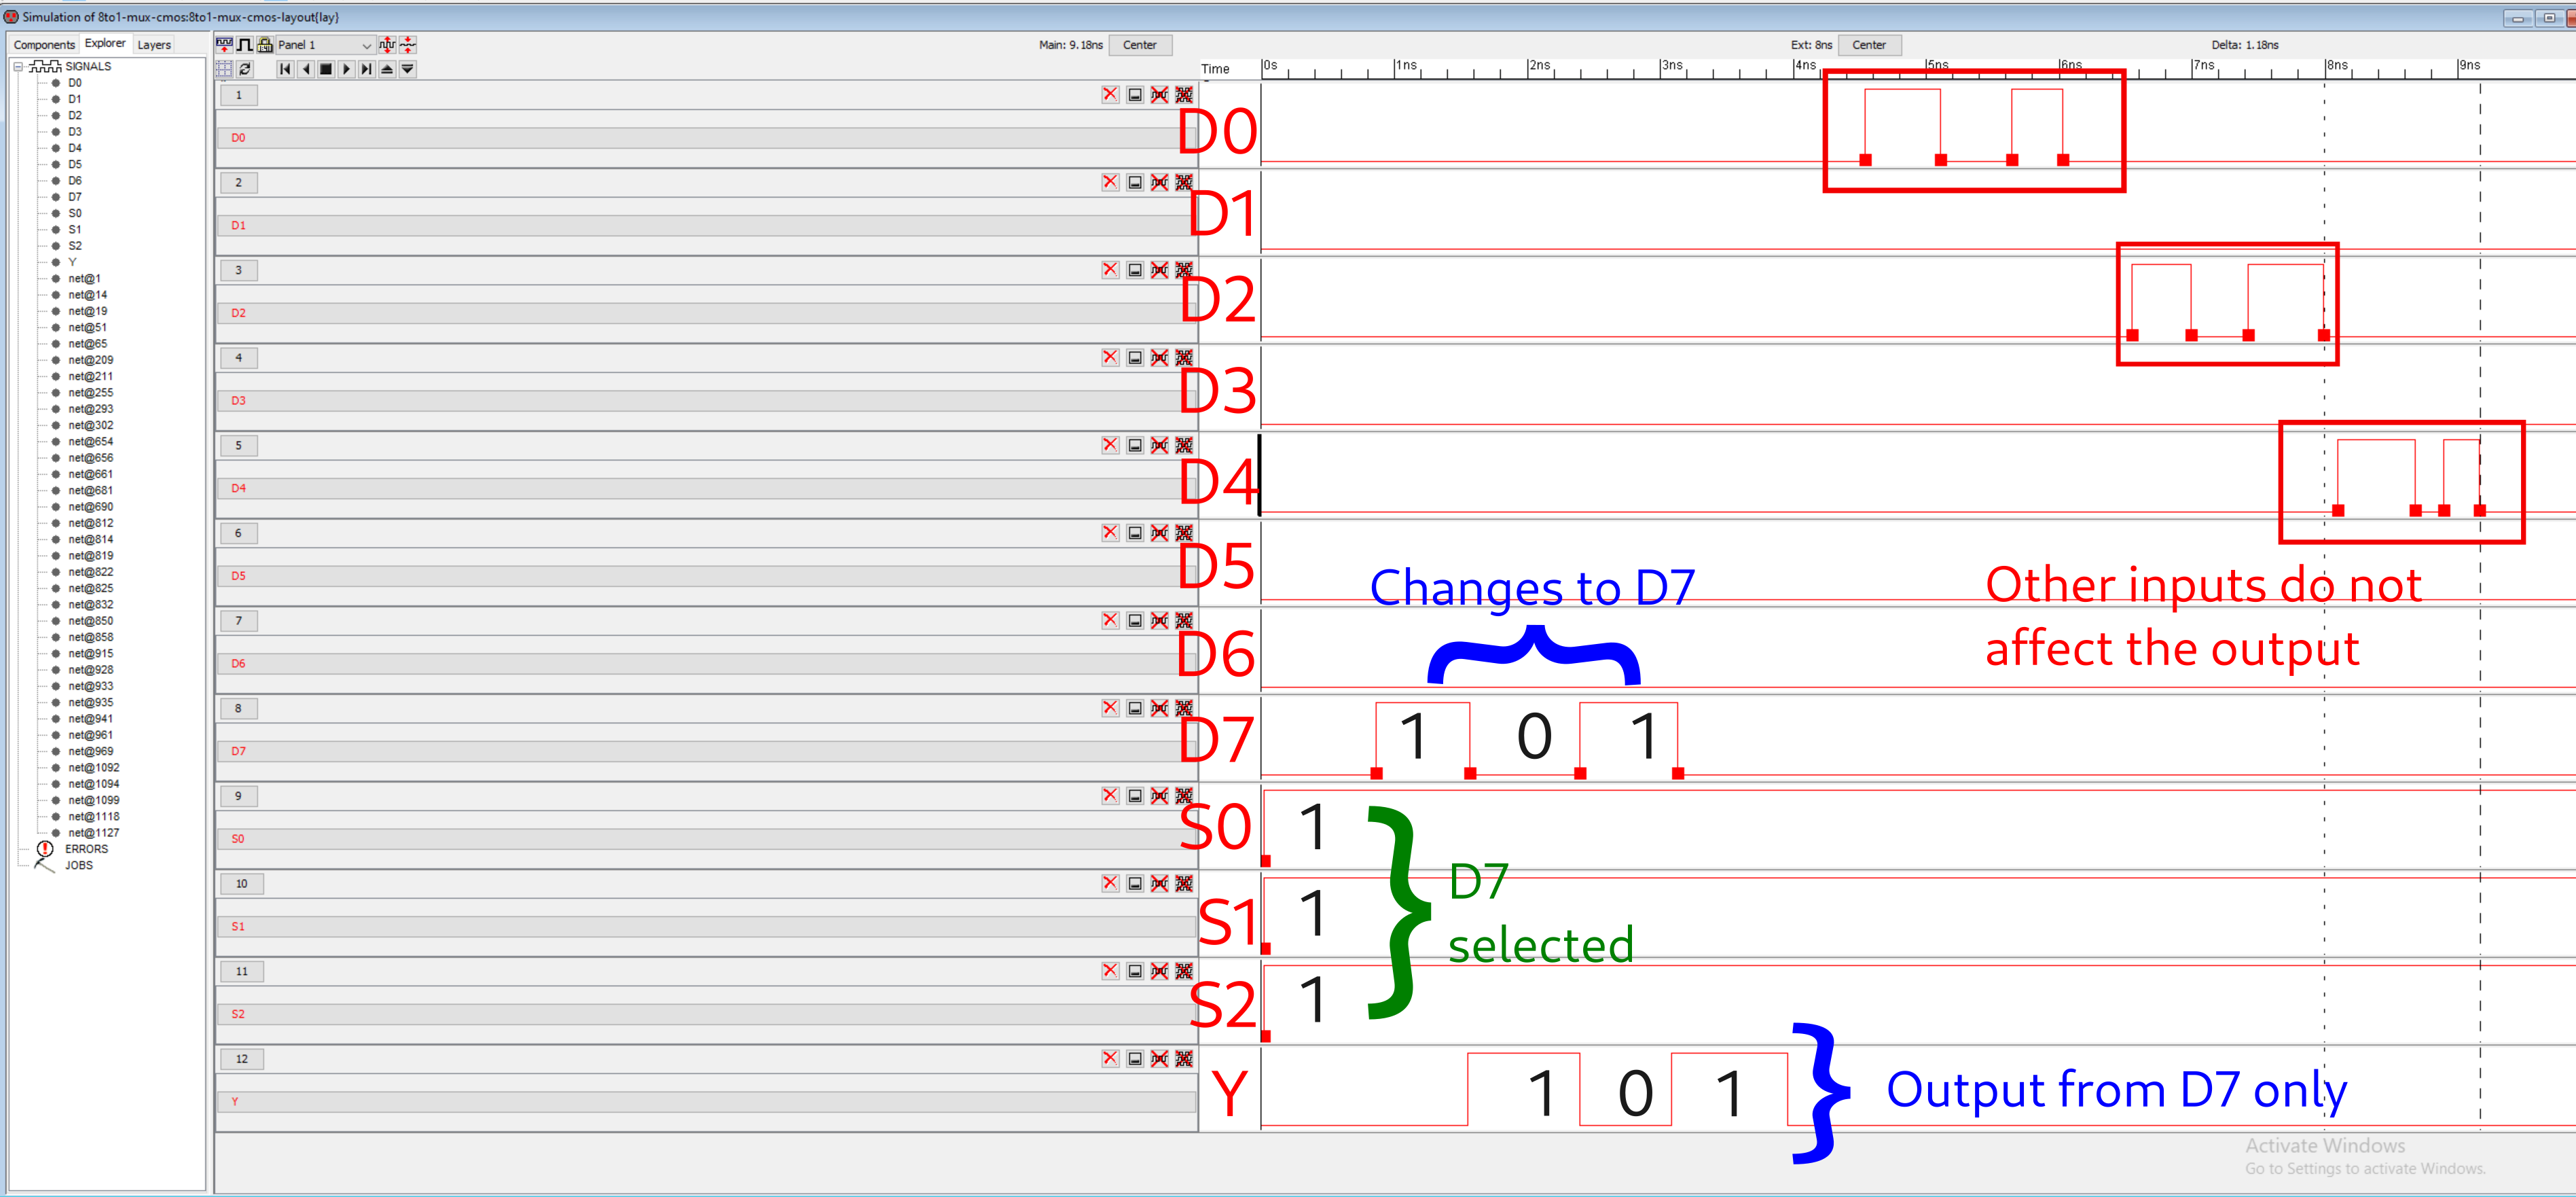
\includegraphics[width=\linewidth, frame]{screenshots/cmos/lay/irsim2.png}
      \caption{Another IRSIM simulation for the CMOS layout showing that the design works as expected.}
      \label{fig:cmoslayirsim2}
    \end{figure}




\section{Schematic vs Layout Measurements}
  \paragraph{}
  This section details the measurements taken for the schematics and layouts of both the transmission gate multiplexer and CMOS multiplexer. The measurements will be compared between the schematic and layout for each. These measurements were taken using the spice code in Figure \ref{fig:meascode} and the measurements were shown for each simulation in the LTSpice sections.

  \subsection{Transmission Gate Schematic vs Layout}
    \paragraph{}
    The measurements for the transmission gate schematic and layout are shown in Table \ref{table:tgmeas}. The table shows that the schematic has shorter rise times than the layout, but the layout has shorter fall times than the schematic. The propagation delay is about double for the layout versus the schematic, and the power draw for the schematic is about four times that of the layout.

    \begin{table}[H]
      \centering
      \footnotesize
      \begin{tabular}{|c|c|c|c|c|}
        \hline
        \textbf{Parameter} & \textbf{TG Schematic} & \textbf{TG Layout}\\
        \hline
        Rise Time & 1.47ns & 4.02ns\\
        \hline
        Fall Time & 7.27ns & 1.29ns\\
        \hline
        $t_{pHL}$ & 273ps & 667ps\\
        \hline
        $t_{pLH}$ & 239ps & 714ps\\
        \hline
        $t_{p}$ & 256ps & 690ps\\
        \hline
        Power Draw & 8.17nW & 2.19nW \\
       \hline
      \end{tabular}
      \caption{The measurement results for the schematic and layout for the transmission gate multiplexer design.}
      \label{table:tgmeas}
    \end{table}

  \subsection{CMOS Schematic vs Layout}
    \paragraph{}
    The measurements for the CMOS schematic and layout are shown in Table \ref{table:cmosmeas}. The rise times, fall times, and propagation delay are shorter for the schematic versus the layout. The power draw for the layout is about double that of the schematic. 



  \begin{table}[H]
    \centering
    \footnotesize
    \begin{tabular}{|c|c|c|c|c|}
      \hline
      \textbf{Parameter} & \textbf{CMOS Schematic} & \textbf{CMOS Layout} \\
      \hline
      Rise Time & 80.8ps & 159ps \\
      \hline
      Fall Time & 39.2ps & 119ps\\
      \hline
      $t_{pHL}$ & 477ps & 793ps\\
      \hline
      $t_{pLH}$ & 357ps & 763ps\\
      \hline
      $t_{p}$ & 417ps & 778ps\\
      \hline
      Power Draw & 473nW & 851nW \\
     \hline
    \end{tabular}
    \caption{The measurements results for the schematic and layout for the CMOS multiplexer design.}
    \label{table:cmosmeas}
  \end{table}

\section{Transmission Gate vs CMOS Measurements}
  \paragraph{}
  All of the measurements taken for the schematics and layouts of both the transmission gate multiplexer and the CMOS multiplexer are shown in Table \ref{table:measurements}. The rise times and fall times for the CMOS design are better by an order of magnitude than the transmission gate design. The propagation delay is only slightly better for the transmission gate design. Where the transmission gate design very clearly outperforms the CMOS design is in power draw. The CMOS design uses two orders of magnitude more power! In terms of area, the transmission gate design is only slightly smaller than the CMOS design, but it still has an advantage. The transmission gate design also has a clear advantage over the CMOS design with 54 transistors versus 72 transistors. 

  \begin{table}[H]
    \centering
    \footnotesize
    \begin{tabular}{|c|c|c|c|c|}
      \hline
      \textbf{Parameter} & \textbf{TG Schematic} & \textbf{TG Layout} & \textbf{CMOS Schematic} & \textbf{CMOS Layout} \\
      \hline
      Rise Time & 1.47ns & 4.02ns & 80.8ps & 159ps \\
      \hline
      Fall Time & 7.27ns & 1.29ns & 39.2ps & 119ps\\
      \hline
      $t_{pHL}$ & 273ps & 667ps & 477ps & 793ps\\
      \hline
      $t_{pLH}$ & 239ps & 714ps & 357ps & 763ps\\
      \hline
      $t_{p}$ & 256ps & 690ps & 417ps & 778ps\\
      \hline
      Power Draw & 8.17nW & 2.19nW & 473nW & 851nW \\
      \hline
      Chip Dimensions ($\lambda$) & N/A & 87$\lambda$ x 429.5$\lambda$ & N/A & 362$\lambda$ x 120$\lambda$ \\
      \hline
      Chip Dimensions ($\mu$m) & N/A & 15.2$\mu$m x 75.2$\mu$m & N/A & 63.4$\mu$m x 21$\mu$m \\
      \hline
      Chip Area($\lambda^2$) & N/A & 37.4$*10^3\lambda^2$ & N/A & 43.4$*10^3\lambda^2$ \\
      \hline
      Chip Area ($\mu$m$^2$) & N/A & 1.14$*10^3\mu$m$^2$ & N/A & 1.33$*10^3\mu$m$^2$ \\
      \hline
      Transistor Count & 54 & 54 & 72 & 72 \\
      \hline
    \end{tabular}
    \caption{The measurement results for the transmission gate schematic and layout as well as the CMOS schematic and layout.}
    \label{table:measurements}
  \end{table}


\section{Conclusion}
  \paragraph{}
  In this project I designed a schematic and layout for an 8-to-1 multiplexer using both transmission gates and CMOS logic. I wrote spice code to simulate the schematics and layouts in order to confirm that they worked properly, and I also wrote spice code to take measurements. I used IRSIM as well to confirm the operation of the designs. After obtaining measurements, I was able to compare the performance between the schematics and layouts and also between the transmission gate and CMOS designs in terms of rise and fall times, propagation delay, power draw, physical size, and transistor count. 

  \paragraph{}
  I learned a lot along the way about turning more complex functions into real functional designs. I also became a lot better at creating layouts, as these designs were much more complex than the XOR gate I designed for the last project. Routing all of the different lines between functional blocks and from inputs proved very challenging, but it felt very rewarding to end up with relatively compact layouts that functioned properly. I also found it interesting to compare the performance between the two designs. Overall, this project was an excellent learning experience, and while it took a very long time, I am pleased with the outcome.

\newpage
\section{References}

\noindent [\text{1}] EE 457 Lectures 1, 2, 3, and 4

\noindent [\text{2}] https://cmosedu.com/videos/electric/tutorial3/electric\_tutorial\_3.htm 

\noindent [\text{3}] https://cmosedu.com/videos/electric/tutorial4/electric\_tutorial\_4.htm 

\noindent [\text{4}] https://en.wikipedia.org/wiki/Multiplexer

\noindent [\text{5}] https://vlsiuniverse.blogspot.com/search/label/8\%3A1\%20mux

\noindent [\text{6}] https://cmosedu.com/videos/electric/tutorial5/electric\_tutorial\_5.htm 























\begin{comment}
%How to do inline code:
\paragraph{}
There is some inline code, \inlinecode{movff STATUS, STATUS\_TEMP}, in this sentence.

This formula $f(x) = x^2$ is an example of inline math.

\end{comment}


\begin{comment}
%How to do equations:

\begin{equation*}
P_{1f_m}=\int^\infty_{-\infty}G_{1f_m}(f)df=0.01\int^\infty_{-\infty}[\delta(f-2700)+\delta(f-2300)]df=0.01*(1+1)=0.02W
\end{equation*}


\end{comment}


\begin{comment}

%Here is a single figure
\begin{figure}[H]
  \centering
  \includegraphics[width=0.9\linewidth, frame]{screenshots/01.png}
  \caption{The system for this lab.}
  \label{fig:01}
\end{figure}

\end{comment}

\begin{comment}

%Here is a double figure
\begin{figure}[H]
  \centering
  \begin{subfigure}[b]{0.45\linewidth}
    \includegraphics[width=\linewidth, frame]{screenshots/02.png}
    \caption{The xyz block.}
  \end{subfigure}
  \begin{subfigure}[b]{0.45\linewidth}
    \includegraphics[width=\linewidth, frame]{screenshots/03.png}
    \caption{The abc block.}
  \end{subfigure}
  \caption{The two figures in this double figure.}
  \label{fig:02}
\end{figure}

\end{comment}


\end{document}
